%%%%%%%%%%%%%%%%%%%%%%%%%%%%%%%%%%%%%%%%%%%%%%%%%%%%%%%%%%%%%%%%%%%%%%%%%%%%%%%%
% Preámbulo                                                                    %
%%%%%%%%%%%%%%%%%%%%%%%%%%%%%%%%%%%%%%%%%%%%%%%%%%%%%%%%%%%%%%%%%%%%%%%%%%%%%%%%

\documentclass[11pt,a4paper,titlepage,twoside,openright,openbib]{report}

\usepackage{estilo_tfg}
\usepackage{rotating}
\setotherlanguage{spanish} % reglas hyphenation

\hypersetup{pdfauthor={Sergio Rodríguez Gayoso},
            pdftitle={Dispositivo e aplicación Android para aumentar a seguridade nos
      desprazamentos en bicicleta},
            pdfsubject={Traballo Fin de Grao},
            pdfkeywords={Seguridade Bicicleta Luces Cámara Vídeo Batería Raspberry Pi Android}}

% Lista de paquetes potencialmente interesantes (uso baixo demanda)

% \usepackage{alltt}       % proporciona o entorno alltt, semellante a verbatim pero que respecta comandos
% \usepackage{enumitem}    % permite personalizar os entornos de lista
% \usepackage{eurofont}    % proporciona o comando \euro
% \usepackage{float}       % permite máis opcións para controlar obxectos flotantes (táboas, figuras)
% \usepackage{hhline}      % permie personalizar as liñas horizontais en arrays e táboas
% \usepackage{longtable}   % permite construir táboas que ocupan máis dunha páxina
% \usepackage{lscape}      % permite colocar partes do documento en orientación apaisada
% \usepackage{moreverb}    % permite personalizar o entorno verbatim
% \usepackage{multirow}    % permite crear celdas que ocupan varias filas da mesma táboa
% \usepackage{pdfpages}    % permite insertar ficheiros en PDF no documento
% \usepackage{rotating}    % permite diferentes tipos de rotacións para figuras e táboas
% \usepackage{subcaption}  % permite a inclusión de varias subfiguras nunha figura
% \usepackage{tabu}        % permite táboas flexibles
% \usepackage{tabularx}    % permite táboas con columnas de anchura determinada

%%%%%%%%%%%%%%%%%%%%%%%%%%%%%%%%%%%%%%%%%%%%%%%%%%%%%%%%%%%%%%%%%%%%%%%%%%%%%%%%
% Corpo                                                                        %
%%%%%%%%%%%%%%%%%%%%%%%%%%%%%%%%%%%%%%%%%%%%%%%%%%%%%%%%%%%%%%%%%%%%%%%%%%%%%%%%

\begin{document}

 %%%%%%%%%%%%%%%%%%%%%%%%%%%%%%%%%%%%%%%%
 % Preliminares do documento            %
 %%%%%%%%%%%%%%%%%%%%%%%%%%%%%%%%%%%%%%%%

 \begin{titlepage}

  \hspace*{128pt}
  \textcolor{udcgray}{{\fontencoding{T1}\fontfamily{phv}\selectfont Departamento de (nome)}}\\[-2pt]
  \hspace*{145pt}
  \textcolor{udcpink}{{\fontencoding{T1}\fontfamily{phv}\selectfont Facultade de Informática}}\\[-32pt]

  \begin{center}
    
\includegraphics[scale=0.3]{imaxes/udc}\\[35pt]

    {\large TRABALLO FIN DE GRAO \\
            GRAO EN ENXEÑERÍA INFORMÁTICA \\
            MENCIÓN EN ENXEÑARÍA DE COMPUTADORES } \\[100pt]

    \begin{huge}
      \bfseries Dispositivo e aplicación Android para aumentar a seguridade nos
desprazamentos en bicicleta \\[7pt]

    \end{huge}
  \end{center}

  \vfill

  \begin{flushright}
    {\large
    \begin{tabular}{ll}
      {\bf Estudante:}        & Sergio Rodríguez Gayoso \\
      {\bf Director/a/es/as:} & Carlos Vázquez Regueiro \\

    \end{tabular}}
  \end{flushright}
  \rightline{A Coruña, \today.}
\end{titlepage}

 \paxinaenbranco
 %\dedicatoria{Dedicatoria}
 %\paxinaenbranco
 %\\paxinaenbranco
 \begin{agradecementos}
 A meus pais polo seu apoio, a meus profesores e director de proxecto pola sua dedicación e paciencia e ao meu colega Carlos pola sua axuda coas probas e vídeos.
 \end{agradecementos}
 \paxinaenbranco
 %%%%%%%%%%%%%%%%%%%%%%%%%%%%%%%%%%%%%%%%%%%%%%%%%%%%%%%%%%%%%%%%%%%%%%%%%%%%%%%%

\begin{abstract}
\thispagestyle{empty}
\blindtext

\vspace*{25pt}
\begin{description}
\item [Palabras chave:] \mbox{} \\[-20pt]
  \begin{itemize}
    \item Seguridade
    \item Bicicleta
    \item Luces
    \item Cámara
    \item Vídeo
    \item Batería
    \item Rasberry Pi
    \item Android
  \end{itemize}
\end{description}

\end{abstract}

%%%%%%%%%%%%%%%%%%%%%%%%%%%%%%%%%%%%%%%%%%%%%%%%%%%%%%%%%%%%%%%%%%%%%%%%%%%%%%%%

 \paxinaenbranco

 \pagenumbering{roman}
 \setcounter{page}{1}

 \tableofcontents \listoffigures
 \listoftables
 \cleardoublepage

 \pagenumbering{arabic}
 \setcounter{page}{1}

 %%%%%%%%%%%%%%%%%%%%%%%%%%%%%%%%%%%%%%%%
 % Capítulos                            %
 %%%%%%%%%%%%%%%%%%%%%%%%%%%%%%%%%%%%%%%%

 \chapter{Introdución}
\label{chap:introducion}

\lettrine{N}{os} últimos anos os medios de transporte alternativos como son o caso de bicicletas, patinetes e similares están aumentando notablemente. As preocupacións medioambientais, os beneficios para a saúde e as vantaxes en termos de custo e eficiencia están a impulsar estes vehículos unipersoais. Porén, a falta de costume dos condutores xunto coas substanciais diferencias entre os vehículos e a falta de proteccións en caso de accidente dificultan a convivencia con automóbiles nas mesmas vías e implican un risco engadido para a integridade física dos condutores destes vehículos. Unha das maneiras de reducir estes riscos é aumentar a visibilidade tanto da bicicleta por parte dos coches coma viceversa co obxectivo de aumentar as distancias e os tempos de reacción dos condutores.

A maioría dos accidentes nos que a vítima é un ciclista implican un turismo na colisión, (referencia dgt 2016) .
O estudo (referencia estudo valencia) con datos da Dirección Xeneral de Tráfico mostra que a pesar de que a maioría de accidentes ciclistas prodúcense de día e con boas condicións de visibilidade, momento no que hay maior número desprazamentos en bicicleta, no caso de accidentes con pouca luminosidade as gravidade das lesión e superior como se mostra na táboa 1.1.


\begin{table}[tb]
    \label{c:lesividade}
    \begin{center}
        \begin{tabular}{|l|l|l|l|l|}
            \hline
             & Morto & Ferido grave & Ferido leve & Total\\ \hline
             Pleno día & 1.1\(\%\)& 13.7\(\%\) & 85.1\(\%\)& 100\(\%\)\\ \hline
             Crepúsculo & 1.9\(\%\) & 13.0\(\%\) &85.1\(\%\) &100\(\%\)\\ \hline
             Iluminación suficiente (noite) &0.7\(\%\) &9.3\(\%\) &90.0\(\%\)  & 100\(\%\)\\ \hline
             Iluminación insuficiente (noite)  & 2.8\(\%\)& 17.7\(\%\)& 79.5\(\%\)& 100\(\%\)\\ \hline
             Sen iluminación (noite) & 10.3\(\%\)& 27.4\(\%\)&62.4\(\%\) & 100\(\%\) \\ \hline
        \end{tabular}
    \end{center}
    \caption{Lesividade en función da luminosidade da vía. (incluir cita) }
    \label{tab:lesividade}
\end{table}

Varios estudos mostran que o uso de luces en bicicletas, especialmente as dinámicas permiten que estas sexan divisadas a maiores distancias tanto de día como de noite. A tese The Nighttime Conspicuity Benefits of Static and Dynamic Bicycle Taillights (incuir cita) estuda os beneficios de diferentes luces traseiras de bicicleta de noite. Conclúe que as luces que se moven co ciclista, como as colocadas nos nocellos, son as que mais visibilidade aportan pero cando o ciclista  deixa de pedalear estes beneficios se perden polo que o uso dunha luz fixa cun patrón de palpadeo pode ser a mellor opción en tódalas circunstancias.

Por outra parte a falta de retrovisores na maioría de bicicletas implica que o ciclista debe xirase cada vez que quere saber o que está a acontecer tras el facendo que así perda momentaneamente a visión do que ocorre diante e incluso o equilibrio en ciclistas non experimentados.

Para paliar estes problemas exponse unha solución baseada nun ou varios dispositivos dotados de luces e cámara xunto a outro de control e visualización.


\section{Obxectivos}
\label{sec:obxectivos}
Os obxectivos principais de este proxecto serán dous:
O primeiro de desenvolvemento de dous dispositivos diferenciados, un dotado de cámara e luces que se poderá colocar en diferentes lugares da bicicleta e do que se poderán utilizar unha ou varias unidades o mesmo tempo que disporá de alimentación propia ou compartida. Un segundo dispositivo de interacción co usuario para o manexo do primeiro e a visualización do vídeo capturado. Tamén será necesario o hardware que permita a comunicación dos dispositivos xa sexa por cable ou sen fíos.

O segundo consistirá en desenvolver o software que permita o funcionamento dos dispositivos. O control das luces para indicar posición aumentar a visibilidade ou indicar manobras coma a freada ou xiro. O control do vídeo permitindo activalo e desactivalo cando se desexe. As posibles automatizacións como o acendido de luces cando haia pouca visibilidade ou a indicación automática da freada. As interfaces de iteración co usuario que permitan o control e a visualización sen distraccións da condución. A integración e comunicación entre os dispositivos en tempo real e de forma transparente para o usuario.

Se comenzará coa análise das posíbeis solucións contemplando as diferentes opcións de hardware dispoñibles tendo en conta o custo, o tamaño, as capacidades de funcionamento, as restricións de compatibilidade, as restricións no software a utilizar, a dispoñibilidade e a dificultade de uso polo usuario final.

Se realizará a implementación da solución elixida e se someterá a probas nun entorno real para comprobar o cumprimento dos requisitos establecidos.


\section{Metodoloxía}
A forma de traballo consistirá en seguir as directrices dadas polo método da enxeñaría partindo de estudo de traballos relacionados anteriores e continuando co análise, deseño implementación e avaliación do sistema implementado.

No apartado de deseño, debido a que o proxecto se estrutura en diferentes compoñentes, optarase por unha metodoloxía Top-Down que consiste en, partindo dos requisitos xerais, dividir o sistema en módulos independentes que se implementarán e probarán por separado. A cada un destes módulos se lle aplicará unha metodoloxía iterativa baseada en prototipos engadindo en cada incremento novas funcionalidades a o prototipo previamente desenvolvido, implementado e validado.

\section{Proposta}
Neste traballo propoñerase unha solución baseada nun microordenador colocado baixo a sela, a Raspberry Pi Zero, que contará cunha cámara é unhas serie de luces leds conectadas. Para o control e a visualización do vídeo en directo realizarase unha aplicación Android que se executará nun teléfono situado no guiador da bicicleta.


\section{Traballo relacionado}
Existen no mercado dispositivos con funcións similares pero poucos integra tódalas funcións. É o caso da cámara Fly6 da compañía Cycliq (incluir referencia), un combo de cámara traseira máis luces que se poden controlar dende o móbil, pero non permite o \emph{streaming} en directo do vídeo, solo a gravación. Conta con características interesantes como a estabilización da imaxe, resistencia a auga e un tamaño moi compacto ou seu prezo e de 179 euros. Outra opción existente é a cámara Hexagon (incluir referencia) que se financiou exitosamente mediante croudfounding no ano 2017 pero non chegou a produción. Este dispositivo si que contaba con \emph{streaming} de vídeo en directo, xunto con acendido automático das luces en caso de freada. A aplicación tamén se encarga de gravar a posición gps no itinerario ou compartila en tempo real, conta cun segundo dispositivo con botóns para o control do dispositivo, e de chegar a producirse o seu prezo estaría entre os 100 e 200 euros.


\section{Estrutura da memoria}
Este documento estrutúrase en seis capítulos e un anexo. Neste primeiro capítulo exponse a motivación os requisitos e as liñas xerais do proxecto. O capítulo 2 explora as posibles alternativas dispoñibles analizando as vantaxes e desvantaxes de cada unha delas fronte a solución elixida. O capítulo 3 relata o proceso e os detalles da implementación do dispositivo a construír xunto co seu software. O capítulo 4 expón a implementación da aplicación Android que se utilizará para o control e a visualización. O capítulo 5 describe as probas realizadas e a análise dos seus resultados. O sexto e derradeiro capítulo recolle as conclusión obtidas trala realización deste proxecto.

 \chapter{Analise e planificación}
\label{chap:Analise e planificación}
Neste capítulo partirase dos requisitos do proxecto para analizar as posibles funcionalidades planificar a implementación e elixir a solución a implantar.

\section{Análise}
O obxetivo do proxecto é a creación de dous dispositivos que realizarán as seguintes funcións:
\begin{itemize}
    \item\textbf{Informar da posición da bicicleta mediante luces}

Esta función realizarase no dispositivo principal. Para elo terá que contar con luces leds e capacidade para controlalas, tamén dispor de capacidade de comunicación co segundo dispositivo e dispoñer dunha fonte de alimentación con capacidade suficiente para facer funcionar as luces.\\

    \item\textbf{Informar das manobras e estado do vehículo mediante luces}

Para realizar esta función os requisitos son os mesmos da función anterior o que engadiremos a necesidade de sensores para detectar cambios no movemento da bicicleta, para sinalizar freadas ou accidentes, e cambios na luz do ambiente para acender as luces cando as condicións lumínicas non sexan favorables.\\

    \item\textbf{Captura de vídeo do que sucede detrás do vehículo}

Esta función tamén se realizará no dispositivo principal e necesitará os requisitos de comunicación e alimentación enerxética xa citados. Contará cunha cámara para capturar as imaxes e necesitará a capacidade para procesalas e transmitilas en tempo real.\\

    \item\textbf{Entrada de ordes do usuario para o control de luces e vídeo}

Esta función se executa no segundo dispositivo, para realizala será necesario un mecanismo de entrada, como poden ser botóns, pulsadores ou pantalla táctil. Tamén se necesitará capacidades de procesamento, comunicación e alimentación enerxética.\\

    \item\textbf{Reprodución do vídeo en tempo real}

Tamén a realizar no dispositivo dous, esta función necesita, a maiores do anteriormente citado unha pantalla na que poder ver o vídeo, e capacidades abondo para reproducilo a tempo real.
\end{itemize}

A maiores destes requisitos funcionais contase cos seguintes obxectivos:
\begin{itemize}
    \item \textbf{Pequeno tamaño e potabilidade}

Co motivo de poder dispoñer o dispositivo da bicicleta, xa sexa para cargalo ou por motivos de seguridade o deixar a bicicleta aparcada na rúa, priorizarase por un deseño portátil. O ideal e que os dispositivos poidan separase da bicicleta con facilidade e que o seu tamaño permita gardalos no peto. Este, xunto cos requisitos funcionais, é o principal motivo polo que optarase por utilizar un telefono móbil como segundo dispositivo, xa que a maioría de persoas dispoñen de un en todo momento, a así evitaríase ter que levar un dispositivo a maiores.

    \item \textbf{Independencia entre dispositivos}

Buscarase que os dispositivos poidan conectarse sen fíos para obter unha maior independencia entre os dispositivos e evitar ter que colocar cables na bicicleta. Tamén se estudará a posibilidade de utilizar unha conexión cableada para diminuír o consumo enerxético dos dispositivos, neste caso optarase preferiblemente por unha conexión USB por compatibilidade co telefono móbil.

    \item \textbf{Batería e alimentación}

Para poder alimentar o dispositivo principal necesitarase dunha batería con capacidade abonda para poder utilizalo polo menos un dia de uso sen ter que recargala. Tamén se estudará a posibilidade de incluír sistemas de aceso e apagado de ser preciso.

    \item \textbf{Sinxeleza e capacidade de actualización}

Pretendese desenvolver un sistema robusto e simple para facilitar o seu mantemento e poder actualizalo de forma sinxela. Especialmente o software ha de ser o mais simple posible para poder permitir incorporar novas funcionalidades no futuro.
\end{itemize}
\section{Planificación}

Seguindo a metodoloxía Top-Dow o desenvolvemento do proxecto dividirase en dúas fases correspondentes a os dous dispositivos. Comezarase polo desenvolvemento do dispositivo principal seguido da aplicación no dispositivo móbil é a comunicación entre ambos. Unha vez desenvolvidas as funcións principais iterarase entre as fase para desenrolar a conexión entre os dispositivos.

\subsection{Fase 1: Dispositivo principal}
As tarefas a realizar son as seguintes:
\begin{itemize}
    \item Conexión dos leds e probas de funcionamento.
    \item Funcións de control dos leds, secuencias e cores.
    \item Servidor de peticións de ordes.
    \item Conexión da cámara e probas de funcionamento.
    \item Transmisión de vídeo.
    \item Autoarranque e apagado.
    \item Alimentación enerxética e batería.
    \item Deseño e construción de carcasa e ancoraxes.
\end{itemize}
\subsection{Fase 2: Aplicación do dispositivo móbil}
Realizaranse a seguintes tarefas:
\begin{itemize}

    \item Introdución de ordes.
    \item Deseño de interfaces.
    \item Transmisión de ordes.
    \item Xestión do estado.
    \item Probas con sensores.
    \item Funcións de automatización.
    \item Recepción de vídeo.
    \item Ancoraxe do dispositivo a bicicleta.
\end{itemize}

\section{Custos do proxecto}
O software utilizado neste proxecto conta con licenzas de software libre polo que os custos restrinxiranse aos recursos humanos e recursos hardware.
Nos recursos hardware da táboa~\ref{tab:custos_hardware} inclúense as pezas utilizadas finalmente para o dispositivo asi como as que se utilizaron para realización de probas. Para aproximar o rango prezos do custo \emph{DIY} de fabricación do dispositivo  na táboa~\ref{tab:custos_dispositivo} calcularanse dúas opción a primeira utilizando os compoñentes máis baratos é a segunda os máis caros.


\begin{table}[tb]
    \label{tab:custos_hardware}
    \caption{Custos monetarios do proxecto}
    \begin{center}
        \begin{tabular}{|l|l|l|l|}
            \hline
             Compoñente & Cantidade & Custo por unidade & Subtotal\\ \hline
             Raspberry Pi Zero W & 2 & 11.00€ & 22.00€ \\ \hline
             Raspberry Pi Zero & 2 & 5.00€ & 5.00€ \\ \hline
             Caixa oficial Pi Zero & 1 & 6.00€ & 6.00€ \\ \hline
             Pi Camera Module V1 & 1 & 5.00€ & 5.00€ \\ \hline
             Pi Camera Module V2 & 2 & 20.00€ & 40.00€ \\ \hline
             Conxunto de lentes & 1 & 2.00€ & 2.00€ \\ \hline
             Tira 8 leds w2812b & 4 & 1.00€ & 4.00€\\ \hline
             Anel 8 leds w2812b & 2 & 1.00€ & 2.00€ \\ \hline
             Adafruit Powerboost 1000C & 1 & 23.00€ & 23.00€ \\ \hline
             Batería Lipo 1600mA & 1 & 7.00€ & 7.00€\\ \hline
             Batería 18650 3400mA & 2 & 2.00€ & 4.00€ \\ \hline
             Material impresión 3D PLA & <1Kg & 15.00€ & 15.00€ \\ \hline
             Cables &  &  & 5.00€ \\ \hline
             Total &  &  & 140.00€ \\ \hline
        \end{tabular}
    \end{center}
\end{table}

\begin{table}[tb]
    \label{tab:custos_dispositivo}
    \caption{Custos de fabricación do dispositivo \emph{DIY}}
    \begin{center}
        \begin{tabular}{|l|l||l|l|}
            \hline
             Menor prezo & Custo  & Maior Prezo & Custo \\ \hline
             Raspberry Pi Zero & 5.00€  & Raspberry Pi Zero W& 11.00€ \\ \hline
             Adaptador Wi-Fi usb & 1.00€ &  & \\ \hline
             Carcasa 3D & 0.50€ & Carcasa ofical & 6.00€ \\ \hline
              &  & Soprte 3D & 0.50€ \\ \hline
             Pi Camera Module V1 & 3.00€ & Pi Camera Module V2 & 20.00€ \\ \hline
              &  & Lentes  & 2.00€ \\ \hline
             8 leds w2812b & 1.00€  &  24 leds w2812b & 3.00€\\ \hline
             Circuito de carga e protección xenérico & 2.00€  & Adafruit Powerboost 1000C & 23.00€ \\ \hline
             Batería Lipo 1600mA & 7.00€ & Batería Lipo 1800mA & 10.00€\\ \hline
             Cables & 1.00€ &  Cables & 1.00€ \\ \hline
             Total & 20.50€ &  Total & 76.50€ \\ \hline
        \end{tabular}
    \end{center}
\end{table}

As estes custos engádense as ferramentas utilizadas incluíndo entre outros ordenador, impresora 3D, multímetro, soldador, dispositivo android e bicicleta.

Na táboa~\ref{tab:custos_humanos} móstranse os recursos humanos utilizados medidos en horas de traballo.

\begin{table}[tb]
    \label{tab:custos_humanos}
    \caption{Tempo empregado no proxecto}
    \begin{center}
        \begin{tabular}{|l|l|}
            \hline
             Tarefa & Tempo\\ \hline
             Documentación & 80h \\ \hline
             Desenvolvemento do dispositivo & 100h \\ \hline
             Desenvolvemento do software do dispositivo & 100h \\ \hline
             Desenvolvemento da aplicación & 200h \\ \hline
             Deseño das pezas 3D & 70h \\ \hline
             Probas e avaliación experimental & 32h\\ \hline
             Total & 512h \\ \hline
        \end{tabular}
    \end{center}
\end{table}

 \chapter{Fundamentos tecnolóxicos}
\label{chap:fundamentos_tecnoloxicos}

\lettrine{N}{este} capítulo esbozase unha arquitectura do sistema e estúdanse as opcións de tecnoloxías dispoñibles para implementalo.

\section{Arquitectura do sistema}

BikeGuard será o nome que asignaremos o sistema e se comporá de dous elementos principais BikeView, o dispositivo de control e visualización e BikeCam o dispositivo de captura de imaxes e sinalización lumínica, plantexarase unha variación de este, BikeLed, que so contará con elementos de iluminación, figura~\ref{fig:bikeguard}.

\begin{figure}[tb]
  \centering
  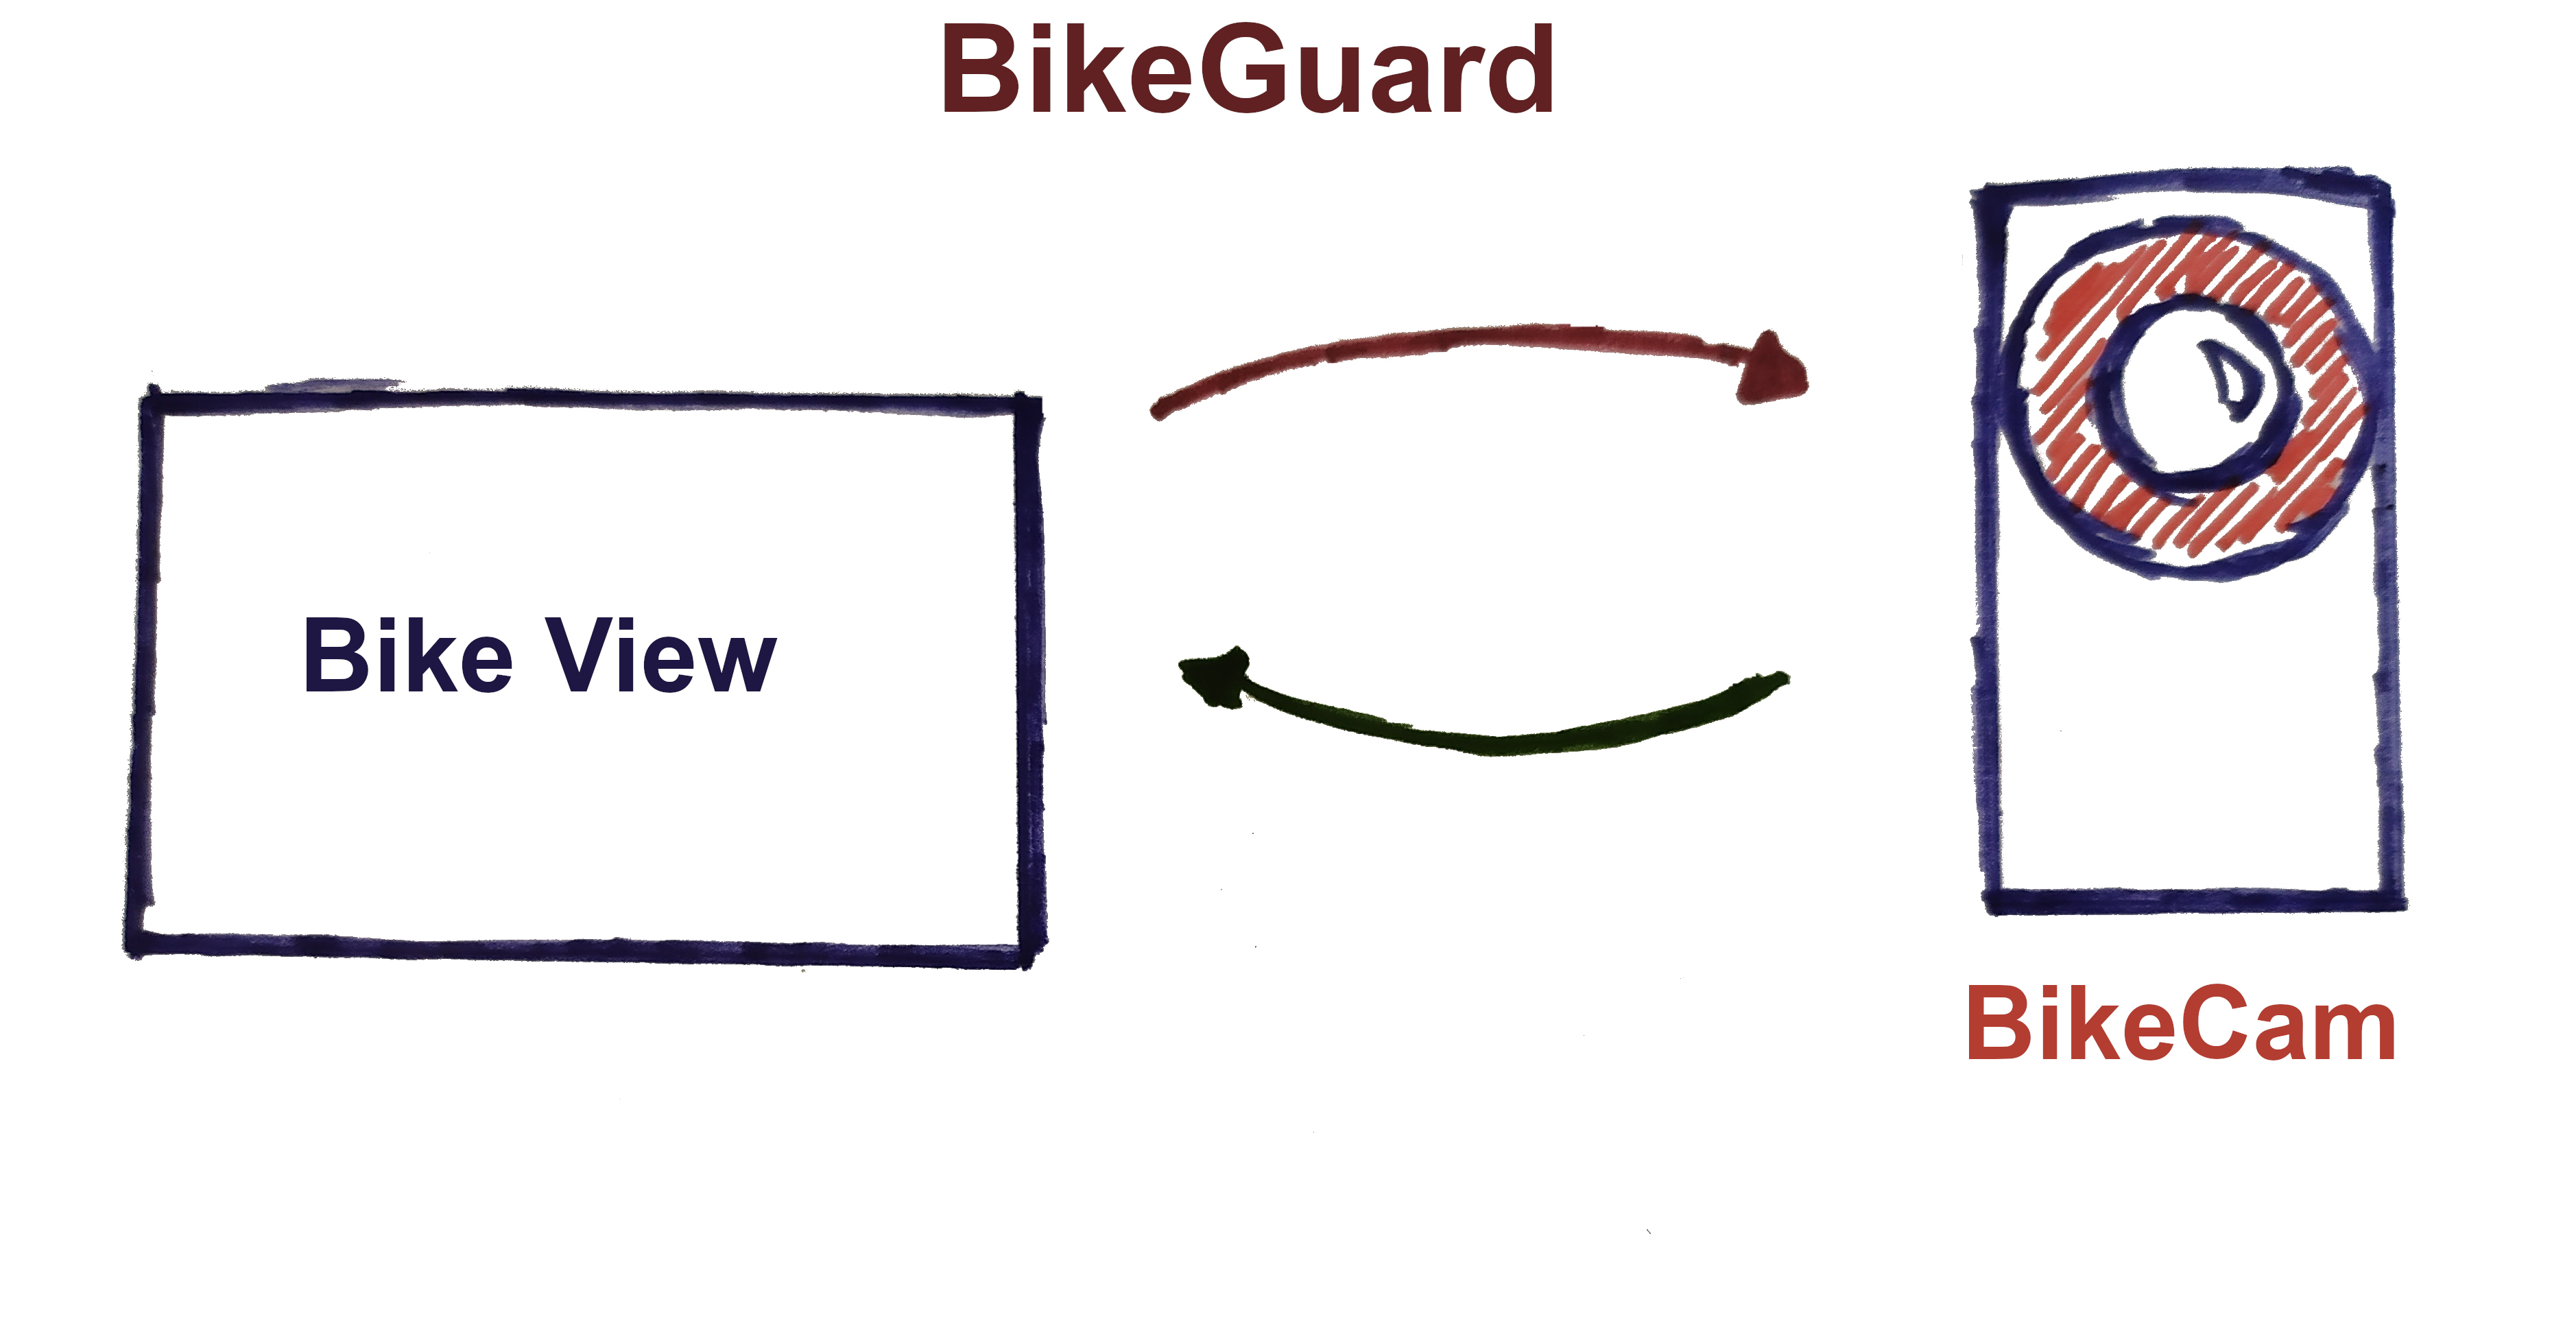
\includegraphics[scale=0.1]{imaxes/bikeguard.jpg}
  \caption{Esquema do sistema BikeGuard.}
  \label{fig:bikeguard}
\end{figure}

Nas seguintes seccións analizaremos as alternativas para o desenvolvemento dos dous dispositivos e as conexións entre ambos.

\section{Esquema xeral de BikeView}

Son moitas as posibilidades de implementación deste dispositivo, os requisitos principais son:
\begin{itemize}
    \item Dispoñer dunha pantalla para visualizar o vídeo e o estado das luces.
    \item Contar con algunha interface de entrada de datos como botóns ou pantalla táctil.
    \item Dispoñer dun hardware para comunicarse co dispositivo principal. Como por exemplo: Wi-Fi, Bluetooth ou USB.
    \item Contar cunha batería ou fonte de alimentación
\end{itemize}

Realizar unha implementación física do dispositivo contaría coas vantaxes de poder contar cunha alta personalización dos seus compoñentes e robustez ao contar cun único hardware obxectivo, unha destas opción sería utilizar un miniordenador como a Rasperry Pi conectado a unha pantalla táctil. Sen embargo optarase outra opción moito máis atractiva: utilizar un telefono móbil e crear unha aplicación dende onde poder visualizar o vídeo e controlar as luces aparte de aforrar a construción do dispositivo. Reducirase así o número de compoñentes que o usuario ten que levar, xa que é habitual dispoñer dun móbil en todo momento.

Desenvolverase a aplicación para o sistema operativo Android xa que este é o sistema operativo máis empregado globalmente e nos permitirá chegar a un maior numero de usuarios.

Para suxeitar un teléfono móbil ao guiador da bicicleta existen múltiples ancoraxes que se adaptan a varios tamaños de teléfono. Tamén existen modelos configurables segundo o tamaño do teléfono que despois se poden imprimir en 3D.

Na figura~\ref{fig:bikeview} mostrase o posible aspecto da aplicación.

\begin{figure}[tb]
  \centering
  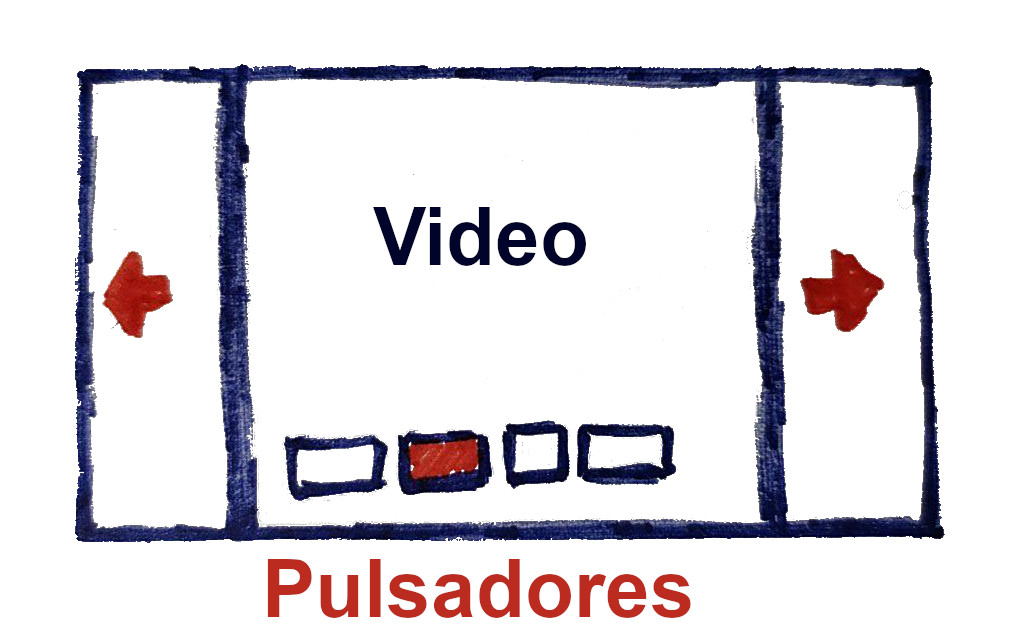
\includegraphics[scale=0.4]{imaxes/bikeview.jpg}
  \caption{Exemplo de implementación de BikeCam.}
  \label{fig:bikeview}
\end{figure}

\section{Esquema xeral de BikeCam}


As esixencias principais destes dispositivo son a existencia de conexións para as luces leds, conexións para unha cámara e capacidade de procesamento e comunicación o que engadiremos unha quinta esixencia, xa que o obxectivo do proxecto e conseguir unha solución de hardware e software libre que posibilite que o usuario final poida adquirir os compoñentes e montalos de forma sinxela, é preciso que os compoñentes sexan fáciles de adquirir e traballar con eles.

A continuación analizaranse as diferentes opción de hardware dispoñibles, as súas características e seus pros e contras para o proxecto proposto.

\subsection{Placas de desenvolvemento}


Sendo o desenvolvemento dunha placa dedicada a este propósito a solución idílica, o custo de este proceso xunto coa dificultade final da construción, sempre que non se optase por unha produción en serie, son as principais contras desta opción. Poren optarase por elixir unha placa cos requisitos requiridos entre as posibles opcións dispoñibles no mercado. Centrarémonos nos modelos co menor tamaño posible.

As placas contempladas son as seguintes:

\begin{itemize}
    \item Arduino

Arduino é unha compañía dedicada o deseño e produción de placas de desenvolvemento con software e hardware, o que permite que terceiras compañías produzan as súas placas permitindo prezos finais de produto moi baixos.

Con un ide propio cunha linguaxe de programación baseada en C++, cunha ampla compatibilidade con diverso hardware, a diversidade de opcións e a sua facilidade de uso converte as súas placas nas máis populares do mercado.

Polo seu tamaño e forma as placas Arduino consideradas son as seguintes:
    \begin{itemize}
        \item Arduino Micro e Arduino Nano

O primeiro esta baseado no microcontrolador de 8bits ATmega32U4 cunha frecuencia de 16MHz, 32KB de memoria flash e 2.5KB de \emph{SRAM}.
Conta con 20 pins de entradas/saídas dixitais con 7 canles \emph{PWM} e 12 pins de entradas analóxicas.

O segundo baséase no microcontrolador de 8bits ATmega328 traballando a unha frecuencia de 16MHz, conta con 32KB de memoria flash e 2KB de \emph{SRAM}. Conta con 22 pins de entradas/saídas dixitais dos cales 6 son \emph{PWM} tamén conta con 8 pins de entradas analóxicas.

Estas dúas versión o contar con gran cantidade de pins tanto dixitais como analóxicos e un consumo enerxético e moi baixo xunto cun baixo prezo inferior os 5 euros nas versións de fabricantes de terceiros fainos perfectos para o propósito de control de leds, pero a sua baixa potencia computacional dificultaría o procesamento de vídeo. Tampouco conta co hardware necesario para as comunicación sen fíos.

        \item Arduino MKR ZERO e Arduino MKR1000

Ambos baseado no procesador ARM M0+ de 32 bit de baixo consumo cunha frecuencia de funcionamento de 48MHz, 256KB de memoria flash e 32kB de \emph{SRAM}, contan con 7 entradas analóxicas e 1 saída analóxica e 12 pins poden funcionar como PWM. Inclúe conexións \emph{SPI} \emph{UART} e \emph{I2C}. Tamén inclúen unha conexión para alimentalos directamente cunha batería de 3.7v. A diferencia entre ambos e que o primeiro conta con 22 pins de entrada e saída dixital mentres que o segundo conta con 8 pero inclúe un chip Wi-Fi.

Ambos teñen as capacidades de procesamento necesarias para a xestión das luces, do vídeo e as conexións. O único punto negativo é que as cámaras compatibles a nivel de conexión e librerías con estas placas non dispoñen de moita calidade de vídeo.

Estas placas poden obterse por entre 20 e 50 euros

        \item Arduino MKR VIDOR 4000

Esta placa de desenvolvemento a parte do procesador ARM M0+ inclúe un chip \emph{FPGA} que permite a sua configuración como diferentes hardware permitido que a placa poda dispoñer de diferentes compoñentes configurables como podería ser múltiples USB ou chips aceleradores de vídeo. Aparte conta con conexión micro HDMI mini PCI Express e un conector de cámara \emph{MIPI} no que se poderían conectar diversas cámara con calidade máis que suficiente para este proxecto.

O seu prezo e superior os 60 euros.
    \end{itemize}
    \item Raspberry Pi

As Raspberry Pi son unha serie de placas de desenvolvemento cun prezo moi axustado e unha potencia suficiente para para pode executar un sistema operativo completo. Grazas a sua popularidade dispón dun amplo soporte e compatibilidade con diversos software e outras plataformas hardware que a fan perfecta para diversos proxectos, como robótica, \emph{IoT} ou centros multimedia.
A versión dispoñible con menor tamaño e a Raspberry Pi Zero
    \begin{itemize}
        \item Raspberry Pi Zero e Raspberry PI Zero W

Esta placa conta cun microprocesador baseado na arquitectura ARM de 32bits que funciona a 1GHz, acompañase de un procesador de vídeo e unha memoria ram de 512MB. No apartado de conexións conta con un micro USB de carga e outro de datos, unha saída de vídeo HDMI e outra analóxica, unha rañura para unha tarxeta micro sd e un conector de cámara CSI. Tamen conta con 20 pins de conexión que a dotan de entradas e saídas dixitais, dúas canles \emph{PWM}, conexiós \emph{SPI} \emph{I2C} e \emph{UART} xunto a conexións de 5v, 3.3v e terra. A versión Zero W tamén dispón dun chip Wi-Fi e Bluetooth.
A sua potencia e capacidade de conexión a fan máis que capaz de para este proxecto, e o seu prezo, 5 e 10 euros respectivamente, é unha das súas principais vantaxes.
    \end{itemize}
    \item ESP8266 e ESP32

A principal característica destas placas é que implementan chips Wi-Fi e Wi-Fi máis Bluetooth respectivamente,contan cun procesador \emph{RISC} de un ou dous núcleos con velocidades dispoñibles entre os 80MHz e 240MHz e memorias ram de entre 32KiB e 520KiB.

Os seus múltiples portos e interfaces,\emph{SPI} ,  \emph{I2C}, \emph{UART}, \emph{PWM} entre outros, o seu baixo consumo e a sua compatibilidade co entorno de programación de arduino fainos ideais para pequenos proxectos de \emph{IoT}, robótica ou domótica. Segundo as súas características poden obterse dende o prezo de un euro.

O igual que pasaba coas placas Arduino os ESP son ideais para a parte do manexo das luces pero non para a xestión do vídeo. Estudarase como opción para a implementación do dispositivo BikeLed.
    \item Outras placas baseadas en procesadores ARM

NO mercado existen múltiples placas de desenvolvemento baseadas en procesadores ARM, non obstante o prezo e o soporte da Raspberry Pi faina a mellor opción para a maioría de proxectos máis xenéricos.
    \item Outras placas baseadas en \emph{FPGA}

Os chip \emph{FPGA} permiten un nivel de personalización hardware moi elevado, pero tamén contan cun alto prezo, e na maioría dos casos cun \emph{toolchain} privativo que e necesario pagar para poder desenvolver en eles. O contrapunto a sua versatilidade é un maior custo de desenvolvemento en comparación con solucións de programación de alto nivel.
\end{itemize}
Tendo en conta o tamaño, a potencia, as conexións dispoñibles e o prezo, decidiuse optar pola Raspberry Pi Zero e Zero W como a placa encargada do control das luces e do vídeo. O dispor esta dunhas características estándar poderíase substituír nun futuro por outro tipo de placa garantido así a modularidade do sistema.

\subsection{Luces led}
As dúas principais vantaxes das luces led fronte a outras formas de iluminación son o se baixo consumo e o seu pequeno tamaño. Estas calidades fainas ideais para un dispositivo portátil coma o que pretendemos construír.
Os requirimentos principais son poder controlar a intensidade dos leds e dispoñer de polo menos un color vermello para indicar a posición e a freada, e un color amarelo ou ámbar para os intermitentes.

Coa intención de miniaturizar se optara por utilizar leds \emph{RGB} que permiten xerar diversas combinacións de cores e así poder utilizar os mesmos leds para as diferentes funcións.
Xa que a Raspberry Pi non conta con saídas analóxicas, utilizaranse as canles \emph{PWM} que permite enviar sinais moduladas en pulsos. A modulación \emph{PWM} permite acender e apagar os leds múltiples veces a unha alta frecuencia a unha velocidade, tan rápidas que o ollo humano percibe como diferentes intensidades lumínicas en función da anchura dos pulsos. En leds \emph{RGB} compatibles o \emph{PWM} tamén se pode utilizar para codificar a cor elixida, e en series de leds conectados e direccionables se pode elixir que led a iluminar e a súa cor e intensidade individualmente, permitindo así controlar un alto numero de leds cunha soa saída \emph{PWM}.

Existen diferentes tipos de leds \emph{RGB} direccionables no mercado, elixiremos o tipo de led en función do seu tipo de conexión, a dispoñibilidade de librerías de software compatibles e coa limitación de que deberán operar a 5v que a voltaxe constante que necesita a Raspberry Pi para funcionar.\\

Os tipos de led direccionables analizados son:
\begin{itemize}
    \item WS2812B e WS2813

Estes leds inclúen un circuíto integrado en cada led que o conectalos en serie permite o control dunha secuencia teoricamente infinita de leds. Cada led conta con tres entradas e tres saídas: voltaxe, terra e datos. A información a pasar os leds se formara cun fluxo de datos a almacenar nun \emph{buffer} en memoria, ocupando a información de cada un 3 bytes, e se pasarán o primeiro led que lerá os primeiros 24 bits coa información da intensidade de cada cor, vermella, verde e azul, e pasará o resto de datos o seguinte led.

Cada led tarda 30 microsegundos en recibir os datos e 50 microsegundos e actualizar a sua cor, o atraso de transmisión entre leds e de 0.5 microsegundos. O consumo máximo de cada led e de 60 mA a 5V.

Os WS2813 engaden unha segunda liña de datos para que se un led deixa de funcionar os seguintes poidan seguir recibindo a información.
    \item SK6812

Estes leds comparten a maioría de características dos WS2812B coa diferencia de que aumenta a sua taxa de refresco a 1.2KHz con respecto os 400Hz dos WS2812B. Tamén engaden unha cuarta cor branca en cada led.

O a nivel de software son compatibles con WS2812B pero as súas diferenzas non permiten a sua interconexión física.
    \item APA102 e APA102C

Estes leds contan cunha interface SPI que conta cunha sinal de datos é outra de reloxo. Isto e para solucionar o problema de sincronización que se poden producir cando os led son manexados dende placas con capacidade de multitarefa sen un \emph{kernel} especifico para entrada e saída a tempo real. Tamén aumenta sua taxa de refresco ata os 19.2kHz.
\end{itemize}

Sendo os leds APA102 superiores en características os outros dous, contan coa desvantaxe de que requiren máis cables de conexión. As súas vantaxes a nivel de velocidade e sincronismo son esencias para a xeración de imaxes ou vídeo pero non para simples animacións como as que utilizaremos neste proxecto. Porén optaremos por utilizar os leds WS2812B e WS2813 ou SK6812.

Este tipo de leds están dispoñibles en diferentes combinacións: leds individuais, tiras flexibles, tiras ríxidas, aneis e matrices. Faremos probas con tiras e aneis de diferentes tamaños.


\subsection{Cámara}

No caso da cámara plantexanse dúas opcións utilizar unha cámara usb ou unha das cámara deseñadas para funcionar coa Raspberry Pi que utilizan a sua conexión \emph{CSI}. Optaremos pola segunda opción xa que unha cámara usb implica un tamaño demasiado grande para o proxecto e ademais non soen estar indicadas para a iluminación de exteriores.

No mercado existen diversos módulos de cámara para a Raspberry Pi pero a maioría están baseados nos Raspberry Pi Camera Module V1 e Raspberry Pi Camera Module V2 a principal diferencia entre ambos e que o primeiro conto con 5 megapixeles mentres o segundo conta con 8 megapixeles e unha notable mellora na calidade de imaxe.\\

As principais diferenzas nos módulos dispoñibles no mercado son:
\begin{itemize}
    \item Tamaño

Existen versións especificas para a Raspberry Pi Zero máis pequenas pero solo do Camera Module V1, as versións normais xa contan cun tamaño moi axustado.

    \item Presenza de filtro infravermello

As cámara soen contar cun filtro de luz infravermella para evitar o \emph{aliassing} que se produce nas cámara xa que as pantallas que utilizamos non están destinadas para emitir infravermellos e os nosos ollos non son capaces de percibilos. As cámaras que non contan con este filtro dan como resultado imaxes máis luminosas e cunha tonalidade violácea. Estas cámara son útiles para entornas exteriores no solpor ou para visión nocturna se se conta con fontes de luz infravermellas.

    \item Tipo de lente

A uso dunha cámara cunha lente curva permite ampliar o campo de visión da cámara, se a lente e demasiado curva se producirá unha distorsión da imaxe nos bordes.

Xa que estas cámaras son todas compatíbeis a nivel de software probaremos diversos tipos con varios tipos de lente xa sexan incorporados ou engadindo unha lente externa.
\end{itemize}




\subsection{Alimentación e baterías}

A Raspberry Pi Zero necesita unha fonte de alimentación que provea de 5V constantes. O seu consumo enerxético varía segundo a carga computacional, o uso do Wi-Fi e o uso da cámara podendo ascender a entorno 300mA.
Os leds tamén funcionarán a 5V cun consumo máximo de 60mA por led, cando emiten luz branca a máxima intensidade.

Plantexamos dúas solución posibles:
\begin{itemize}
    \item Bateria externa USB

Utilizar unha batería usb externa permite dispoñer de altas capacidades que prolongarían o tempo de uso pero implican o uso dun dispositivo a maiores. Outra de desvantaxes e que cando se esgote a batería a corrente interrompese de golpe sen que a Raspberry poida realizar un apagado normal, como consecuencia tras varios apagados podería danarse o sistema de ficheiros se se estaba a escribir nel no momento do apagado.

    \item Batería, circuíto de alimentación e circuíto de acendido e apagado.

A maioría de baterías usadas en electrónica son baterías de \emph{ions de litio} principalmente devido as sua alta capacidade enerxética e lonxevidade. A \emph{voltaxe nominal} destas baterías e de 3.7V sendo 4.2V a voltaxe coa carga o máximo e por debaixo de 3V deixan de proporcionar suficiente intensidade eléctrica para a maioría de aplicacións. Este tipo de baterías son as que atoparemos nos teléfonos móbiles, ordenadores portátiles e incluso en vehículos eléctricos. Poden colocarse en serie cando e necesario unha maior voltaxe ou en paralelo cando o que se necesita e unha maior capacidade.

Para poder utilizar estas baterías é necesario un circuíto de carga, un de protección, e un de conversión de voltaxe. Na maioría dos casos as batería de consumo utilizan o estándar USB, que funciona a 5V, tanto para cargarse como para proporcionar enerxía. Polo que será necesario un chip de carga que acepte unha toma de 5V e que cargue a batería ata 4.2V. As baterías de litio poden ser perigosas danándose e chegando incluso a estoupar se se descargan demasiado ou se se sobrecargan polo que é necesario un circuíto de protección que evite a sobrecarga e a sobrecarga. Para proporcionar unha saída estable de 5V tamén é necesario un conversor de voltaxe.
É habitual atopar o circuítos de carga máis protección xuntos no mesmo chip aínda que tamén se atopan circuítos que integran as tres funcionalidades.
\end{itemize}
\subsection{Software a utilizar}
A Raspberry Pi conta cunha ampla gama de sistemas operativos, algúns con propósitos concretos como reprodución de multimedia, servidores locais ou nodos de rede. Tamén conta con versións das distribucións Linux máis popular como Ubuntu, Arch ou Kali entre outros.
Raspbian é unha distribución baseada en Debian, é máis antiga e máis optimizada para a Raspberry Pi e a que dispón de máis soporte polo que será a elixida para o proxecto.

Para o control dos leds existen varias librarías dispoñibles para varias linguaxes de programación. As máis utilizadas son a de Adafruit, que só está dispoñible en Python, e a de Jeremy Garff que será a que utilicemeos, xa que conta con unha documentación detallada e esta dispoñible en varias linguaxes de programación, entre outras C, Python e Java.

Para a captura e transmisión do vídeo contamos con varias alternativas. A libraría \emph{picamera} para Python permite configurar calquera parámetro e o \emph{streaming} do vídeo na rede. Por outra parte o software para captura de vídeo \emph{raspivideo}, escrito en Python, tamén permite moitos parámetros de configuración é a sua saída de vídeo pode enviarse a rede utilizando algún programa para redirecionar o \emph{bitstream} dos datos como pode ser o software \emph{socat}.

A comunicación entre o dispositivo de control e o de luces e captura de vídeo realizarase a través dunha conexión IP. Para manexar as peticións podemos empregar unha das clases servidor Python, unha libraría de terceiros ou implementar o servidor a nivel de \emph{sockets}.

Por motivos de compatibilidade entre todo o software necesitado para o control de leds, vídeo, e conexións, decidiremos integralo todo nunha aplicación Python que se encargará das tres tarefas.

\subsection{Caixa e ancoraxes a bicicleta}


O lugar a colocar o dispositivo de iluminación e captura será na barra da sela da bicicleta, esta posición é a ideal tanto para capturar o vídeo como para que as luces sexan vistas polo tráfico que circula detrás do vehículo.

A Raspberry Pi conta cunha caixa oficial na que se pode instalar xunto coa cámara V2. Esta é a que utilizaremos no caso de alimentala cunha batería externa. Para suxeitar a placa á barra deseñaremos un soporte e o imprimiremos cunha impresora 3D. Para a versión con batería interna deseñaremos unha caixa protectora que albergue tódolos compoñentes e que se poida suxeitar á barra.

Os prototipos imprimiranse en \emph{PLA} un material biodegradable e de fácil impresión, no é o mellor material para resistir a auga ou a humidade pero é ideal para o prototipado. Poderá utilizarse \emph{ABS} para imprimir unha versión final, un material moito máis resistente as condicións atmosféricas.

\subsection{Esquema conceptual de BikeCam}

As decisións tomadas condúcenos a un dispositivo composto por unha Raspberry Pi Zero con presenza de batería interna ou externa e unha o varias tiras LED RGB, na figura~\ref{fig:bikecam} mostrase unha posible aproximación incluíndo unha Raspberry Pi Zero W unha Pi Camera V1 e unha tira e un anel WS2812 de 8 luces cada un.
\begin{figure}[tb]
  \centering
  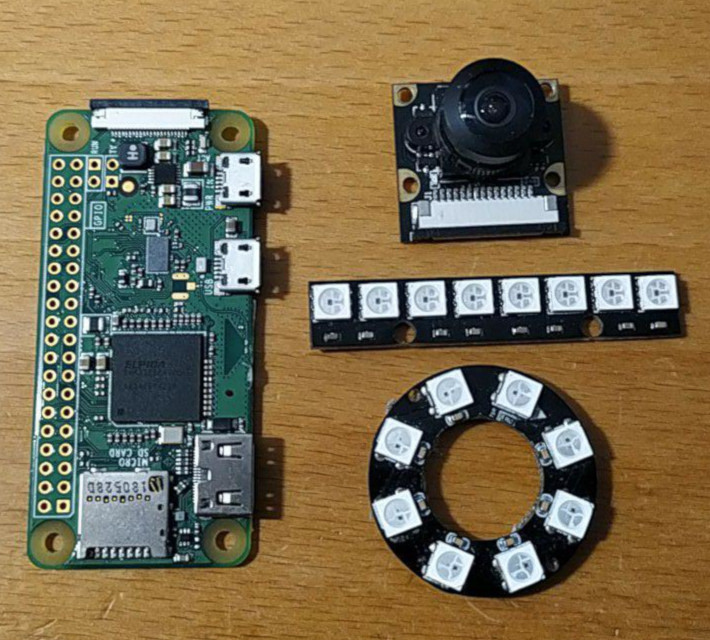
\includegraphics[scale=0.4]{imaxes/bikecam.jpg}
  \caption{Exemplo de implementación de BikeCam.}
  \label{fig:bikecam}
\end{figure}
\subsection{Esquema conceptual de BikeLed}

Este dispositvio cotaría con un Arduino Nano mais un chip Wi-Fi ou Bluetooth ou cun ESP32 conectado a unhas tiras Leds RGB e unhas Batería, na foto da figura~\ref{fig:bikeled} mostras unha imaxe dos posibles compoñenetes que poderia implemtear, con un anel RGB de 8 luces, unha bateria de 400mA e un microcontrolador ESP8266 Wemmos D1 mini con Wi-Fi.
\begin{figure}[tb]
  \centering
  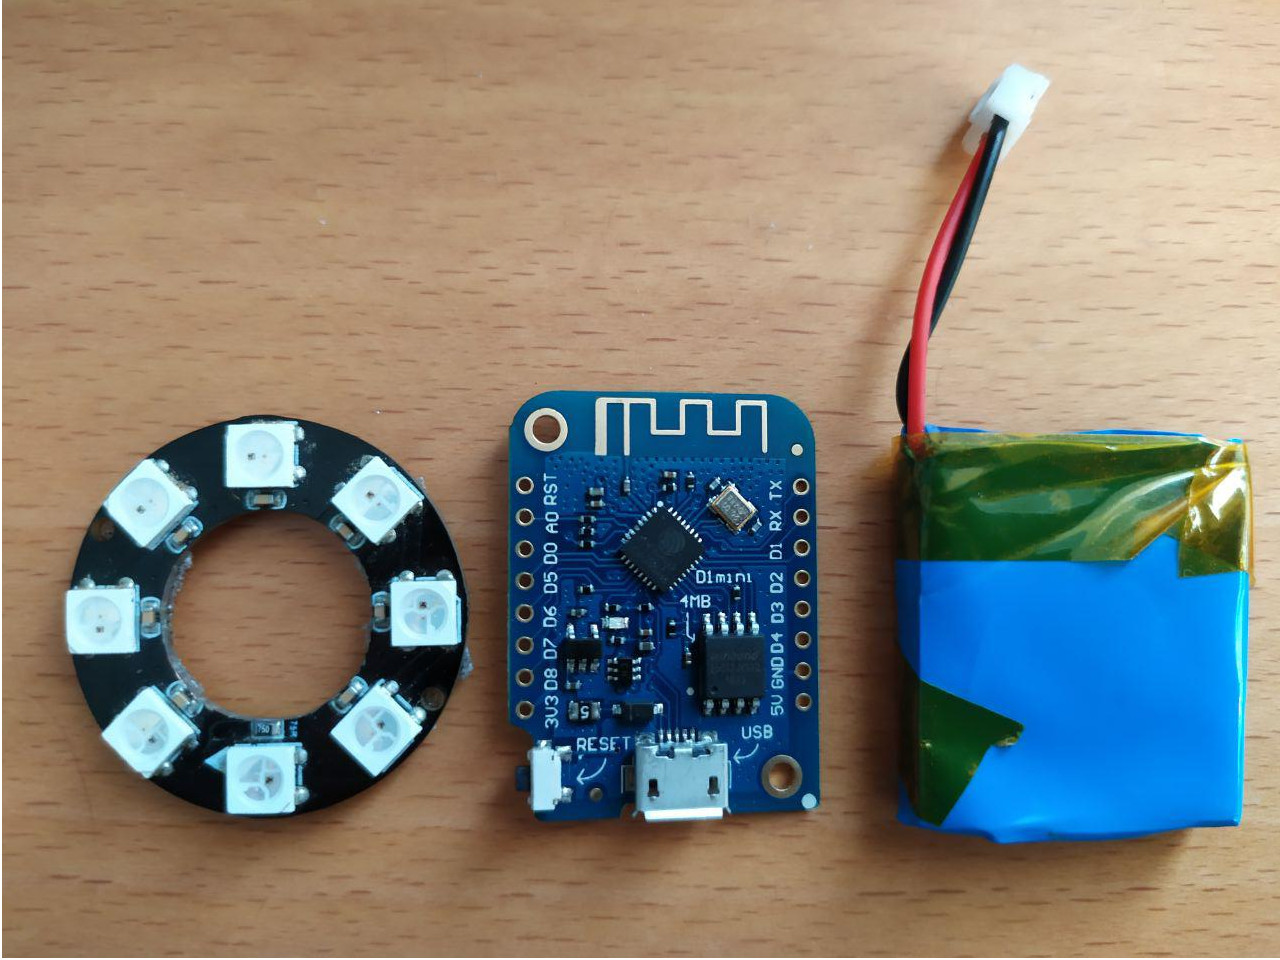
\includegraphics[scale=0.3]{imaxes/bikeled.jpg}
  \caption{Exemplo de implementación de BikeLed.}
  \label{fig:bikeled}
\end{figure}

\section{Comunicacións entre BikeCam e BikeView}
Optarase por utilizar un sistema de conexión cliente servidor no que BikeView realizará peticións o servidor en BikeCam que responderá actuando as luces e devolvendo cofirmacións e a sinal de vídeo.



\subsection{Canle de comunicaións}
Partindo da elección da Raspebrry Pi para BikeCam e un dispositivo Android para BikeView as opcións para a implementación física da conexión son as seguintes.
begin{\begin{itemize}
  \item USB

  A Raspberry Pi Zero conta cun conector USB 2.0, e os dispositivos Android implementan este estándar ou o superior 3.0 polo que a velocidade máxima será restrinxida pola Raspberry Pi permitindo un máximo de 480Mbits/s esta velocidade permitiría a transimisión de vidio sen problemas.
  Tanto no dispositivo Android como na Raspberry Pi pódese implementar unha conexión Ethernet virtual sobre USB o que facilitaría a estandarización das comunicacións.

  Unha das principais vantaxes de usar unha conexión USB é que poderíase alimentar enerxeticamente o dispositivo BikeCam dende BikeView sempre e cando o consumo de este non supere o máximo de 500mA que pode subministrar un dispositivo Android por USB en modo OTG.

  A principal desvantaxe é a necesidade de ter un cable unindo ambos dispositivos dende o guiador a sela da bicicleta.

  \item WI-Fi

  A Raspberry Pi Zero conta con un chip WI-Fi 802.11n e calquera móbil actual implementan esta versión do estándar ou unha superior. Este estandar Wi-Fi permite unha velocidade máxima de transmisión de 300Mbits/s tamén neste caso suficiente para a transmisión de vídeo HD.

  A principal vantaxe do uso do WI-Fi é a independencia dos dispositivos pero coma contrapartida será necesario que BikeCam conte cunha batería propia.

  \item Bluetooth

  Bluetooth 4.0 é a versión do estándar implemetado pola Rasberry Pi Zero W e neste caso tamén marcará a velocidade máxima de transmisión xa que os dispositivos Android actuais implementan versións iguales ou superiores do estándar.Esta velocidade será 25Mbits/s o que non nos permitiría transmitir vídeo en tempo real. Sen embargo esta conexión e máis que suficiente para o dispositivo BikeLed que non require transmisión de vídeo.

  Unha das súas vantaxes fronte o Wi-Fi e menor consumo enerxético.
\end{itemize}

Tendo en conta a viabilidade das tres opción optarase por a implementación das conexión a través de Wi-Fi xa que é a opción que menos limitacións carrexa. Neste caso optarase por usar modo \emph{hotspot} de Android no que o dispositvo BikeView xerará unha rede Wi-Fi a que se conectará io dispositivo BikeCam.

\subsection{Protocolos de comunicación}
Como o esquema de comunicacións involucra so a dous dispositivos intentarase realizar un esquema de comunicación o máis sinxelo posible. Será o dispositvo BikeLed o que exerza de servido e escoite as ordes enviadas dende BikeView, para elo a primeira aproximación foi a creación dun servidor \emph{http} pero como non requiríamos da necesidade de utilizar múltiples threads decidiuse facer unha aproximación de mais simple, implementar un protocolo de envío de ordes a través de paquetes \emph{UDP} no que o dispositivo BikeView enviará ordes de control e ordes para saber se o sistema segue activo, e o servidor de BikeCam responderá se se recibiu a orde.

\subsection{Protocolos de videostreaming}
Existen varias opcións para transmitir vídeo a trabes da rede pero moi poucas están orientadas a transmisión de vídeo en tempo real e as que o conseguen e a base de reducir a calidade do vídeo.

As opcións que maior velocidade prometen son aquelas que transmiten o vídeo capturado en formato H.264 directamente, redireccionando o fluxo da cámara a rede en paquetes \emph{UDP}. No capítulo de Deseño e implementación do dispositivo detallaranse a probas realizas a diferentes software para obter a menor latencia de transmisión.

Para a recepción realizado no dispositivo BikeView levaremos a cabo a descompresión a baixo nivel descompoñendo os paquetes recibidos e enviando os fotogramas a superficie de vídeo.

 \chapter{Deseño e implementación do dispositivo}
\label{chap:implementacion_dispositivo}
Neste capítulo afondarase no desenvolvemento do dispositivo comezando polo aspecto físico, opcións dispoñibles e alternativas, seguido pola construción do dispositivo e a implementación do sofware tendo en conta os problemas xurdidos e as solucións aplicadas.


\section{Esquema xeral do dispositivo HW}


As esixencias principais destes dispositivo son a existencia de conexións para as luces leds, conexións para unha cámara e capacidade de procesamento e comunicación o que engadiremos unha quinta esixencia, xa que o obxectivo do proxecto e conseguir unha solución de hardware e software libre que posibilite que o usuario final poida adquirir os compoñentes e montalos de forma sinxela, é preciso que os compoñentes sexan fáciles de adquirir e traballar con eles.

A continuación analizaranse as diferentes opción de hardware dispoñibles, as súas características e seus pros e contras para o proxecto proposto.

\subsection{Placas de desenvolvemento}


Sendo o desenvolvemento dunha placa dedicada a este propósito a solución idílica, o custo de este proceso xunto coa dificultade final da construción, sempre que non se optase por unha produción en serie, son as principais contras desta opción. Poren optarase por elixir unha placa cos requisitos requiridos entre as posibles opcións dispoñibles no mercado. Centrarémonos nos modelos co menor tamaño posible.

As placas contempladas son as seguintes:

\begin{itemize}
    \item Arduino

Arduino é unha compañía dedicada o deseño e produción de placas de desenvolvemento con software e hardware, o que permite que terceiras compañías produzan as súas placas permitindo prezos finais de produto moi baixos.

Con un ide propio cunha linguaxe de programación baseada en C++, cunha ampla compatibilidade con diverso hardware, a diversidade de opcións e a sua facilidade de uso converte as súas placas nas máis populares do mercado.

Polo seu tamaño e forma as placas Arduino consideradas son as seguintes:
    \begin{itemize}
        \item Arduino Micro e Arduino Nano

O primeiro esta baseado no microcontrolador de 8bits ATmega32U4 cunha frecuencia de 16MHz, 32KB de memoria flash e 2.5KB de \emph{SRAM}.
Conta con 20 pins de entradas/saídas dixitais con 7 canles \emph{PWM} e 12 pins de entradas analóxicas.

O segundo baséase no microcontrolador de 8bits ATmega328 traballando a unha frecuencia de 16MHz, conta con 32KB de memoria flash e 2KB de \emph{SRAM}. Conta con 22 pins de entradas/saídas dixitais dos cales 6 son \emph{PWM} tamén conta con 8 pins de entradas analóxicas.

Estas dúas versión o contar con gran cantidade de pins tanto dixitais como analóxicos e un consumo enerxético e moi baixo xunto cun baixo prezo inferior os 5 euros nas versións de fabricantes de terceiros fainos perfectos para o propósito de control de leds, pero a sua baixa potencia computacional dificultaría o procesamento de vídeo. Tampouco conta co hardware necesario para as comunicación sen fíos.

        \item Arduino MKR ZERO e Arduino MKR1000

Ambos baseado no procesador ARM M0+ de 32 bit de baixo consumo cunha frecuencia de funcionamento de 48MHz, 256KB de memoria flash e 32kB de \emph{SRAM}, contan con 7 entradas analóxicas e 1 saída analóxica e 12 pins poden funcionar como PWM. Inclúe conexións \emph{SPI} \emph{UART} e \emph{I2C}. Tamén inclúen unha conexión para alimentalos directamente cunha batería de 3.7v. A diferencia entre ambos e que o primeiro conta con 22 pins de entrada e saída dixital mentres que o segundo conta con 8 pero inclúe un chip Wi-Fi.

Ambos teñen as capacidades de procesamento necesarias para a xestión das luces, do vídeo e as conexións. O único punto negativo é que as cámaras compatibles a nivel de conexión e librerías con estas placas non dispoñen de moita calidade de vídeo.

Estas placas poden obterse por entre 20 e 50 euros

        \item Arduino MKR VIDOR 4000

Esta placa de desenvolvemento a parte do procesador ARM M0+ inclúe un chip \emph{FPGA} que permite a sua configuración como diferentes hardware permitido que a placa poda dispoñer de diferentes compoñentes configurables como podería ser múltiples USB ou chips aceleradores de vídeo. Aparte conta con conexión micro HDMI mini PCI Express e un conector de cámara \emph{MIPI} no que se poderían conectar diversas cámara con calidade máis que suficiente para este proxecto.

O seu prezo e superior os 60 euros.
    \end{itemize}
    \item Raspberry Pi

As Raspberry Pi son unha serie de placas de desenvolvemento cun prezo moi axustado e unha potencia suficiente para para pode executar un sistema operativo completo. Grazas a sua popularidade dispón dun amplo soporte e compatibilidade con diversos software e outras plataformas hardware que a fan perfecta para diversos proxectos, como robótica, \emph{IoT} ou centros multimedia.
A versión dispoñible con menor tamaño e a Raspberry Pi Zero
    \begin{itemize}
        \item Raspberry Pi Zero e Raspberry PI Zero W

Esta placa conta cun microprocesador baseado na arquitectura ARM de 32bits que funciona a 1GHz, acompañase de un procesador de vídeo e unha memoria ram de 512MB. No apartado de conexións conta con un micro USB de carga e outro de datos, unha saída de vídeo HDMI e outra analóxica, unha rañura para unha tarxeta micro sd e un conector de cámara CSI. Tamen conta con 20 pins de conexión que a dotan de entradas e saídas dixitais, dúas canles \emph{PWM}, conexiós \emph{SPI} \emph{I2C} e \emph{UART} xunto a conexións de 5v, 3.3v e terra. A versión Zero W tamén dispón dun chip Wi-Fi e Bluetooth.
A sua potencia e capacidade de conexión a fan máis que capaz de para este proxecto, e o seu prezo, 5 e 10 euros respectivamente, é unha das súas principais vantaxes.
    \end{itemize}
    \item ESP8266 e ESP32

A principal característica destas placas é que implementan chips Wi-Fi e Wi-Fi máis Bluetooth respectivamente,contan cun procesador \emph{RISC} de un ou dous núcleos con velocidades dispoñibles entre os 80MHz e 240MHz e memorias ram de entre 32KiB e 520KiB.

Os seus múltiples portos e interfaces,\emph{SPI} ,  \emph{I2C}, \emph{UART}, \emph{PWM} entre outros, o seu baixo consumo e a sua compatibilidade co entorno de programación de arduino fainos ideais para pequenos proxectos de \emph{IoT}, robótica ou domótica. Segundo as súas características poden obterse dende o prezo de un euro.

O igual que pasaba coas placas Arduino os ESP son ideais para a parte do manexo das luces pero non para a xestión do vídeo.
    \item Outras placas baseadas en procesadores ARM

NO mercado existen múltiples placas de desenvolvemento baseadas en procesadores ARM, non obstante o prezo e o soporte da Raspberry Pi faina a mellor opción para a maioría de proxectos máis xenéricos.
    \item Outras placas baseadas en \emph{FPGA}

Os chip \emph{FPGA} permiten un nivel de personalización hardware moi elevado, pero tamén contan cun alto prezo, e na maioría dos casos cun \emph{toolchain} privativo que e necesario pagar para poder desenvolver en eles. O contrapunto a sua versatilidade é un maior custo de desenvolvemento en comparación con solucións de programación de alto nivel.
\end{itemize}
Tendo en conta o tamaño, a potencia, as conexións dispoñibles e o prezo, decidiuse optar pola Raspberry Pi Zero e Zero W como a placa encargada do control das luces e do vídeo.

\subsection{Luces led}
As dúas principais vantaxes das luces led fronte a outras formas de iluminación son o se baixo consumo e o seu pequeno tamaño. Estas calidades fainas ideais para un dispositivo portátil coma o que pretendemos construír.
Os requirimentos principais son poder controlar a intensidade dos leds e dispoñer de polo menos un color vermello para indicar a posición e a freada, e un color amarelo ou ámbar para os intermitentes.

Coa intención de miniaturizar se optara por utilizar leds \emph{RGB} que permiten xerar diversas combinacións de cores e así poder utilizar os mesmos leds para as diferentes funcións.
Xa que a Raspberry Pi non conta con saídas analóxicas, utilizaranse as canles \emph{PWM} que permite enviar sinais moduladas en pulsos. A modulación \emph{PWM} permite acender e apagar os leds múltiples veces a unha alta frecuencia a unha velocidade, tan rápidas que o ollo humano percibe como diferentes intensidades lumínicas en función da anchura dos pulsos. En leds \emph{RGB} compatibles o \emph{PWM} tamén se pode utilizar para codificar a cor elixida, e en series de leds conectados e direccionables se pode elixir que led a iluminar e a súa cor e intensidade individualmente, permitindo así controlar un alto numero de leds cunha soa saída \emph{PWM}.

Existen diferentes tipos de leds \emph{RGB} direccionables no mercado, elixiremos o tipo de led en función do seu tipo de conexión, a dispoñibilidade de librerías de software compatibles e coa limitación de que deberán operar a 5v que a voltaxe constante que necesita a Raspberry Pi para funcionar.\\

Os tipos de led direccionables analizados son:
\begin{itemize}
    \item WS2812B e WS2813

Estes leds inclúen un circuíto integrado en cada led que o conectalos en serie permite o control dunha secuencia teoricamente infinita de leds. Cada led conta con tres entradas e tres saídas: voltaxe, terra e datos. A información a pasar os leds se formara cun fluxo de datos a almacenar nun \emph{buffer} en memoria, ocupando a información de cada un 3 bytes, e se pasarán o primeiro led que lerá os primeiros 24 bits coa información da intensidade de cada cor, vermella, verde e azul, e pasará o resto de datos o seguinte led.

Cada led tarda 30 microsegundos en recibir os datos e 50 microsegundos e actualizar a sua cor, o atraso de transmisión entre leds e de 0.5 microsegundos. O consumo máximo de cada led e de 60 mA a 5V.

Os WS2813 engaden unha segunda liña de datos para que se un led deixa de funcionar os seguintes poidan seguir recibindo a información.
    \item SK6812

Estes leds comparten a maioría de características dos WS2812B coa diferencia de que aumenta a sua taxa de refresco a 1.2KHz con respecto os 400Hz dos WS2812B. Tamén engaden unha cuarta cor branca en cada led.

O a nivel de software son compatibles con WS2812B pero as súas diferenzas non permiten a sua interconexión física.
    \item APA102 e APA102C

Estes leds contan cunha interface SPI que conta cunha sinal de datos é outra de reloxo. Isto e para solucionar o problema de sincronización que se poden producir cando os led son manexados dende placas con capacidade de multitarefa sen un \emph{kernel} especifico para entrada e saída a tempo real. Tamén aumenta sua taxa de refresco ata os 19.2kHz.
\end{itemize}

Sendo os leds APA102 superiores en características os outros dous, contan coa desvantaxe de que requiren máis cables de conexión. As súas vantaxes a nivel de velocidade e sincronismo son esencias para a xeración de imaxes ou vídeo pero non para simples animacións como as que utilizaremos neste proxecto. Porén optaremos por utilizar os leds WS2812B e WS2813 ou SK6812.

Este tipo de leds están dispoñibles en diferentes combinacións: leds individuais, tiras flexibles, tiras ríxidas, aneis e matrices. Faremos probas con tiras e aneis de diferentes tamaños.


\subsection{Cámara}

No caso da cámara plantexanse dúas opcións utilizar unha cámara usb ou unha das cámara deseñadas para funcionar coa Raspberry Pi que utilizan a sua conexión \emph{CSI}. Optaremos pola segunda opción xa que unha cámara usb implica un tamaño demasiado grande para o proxecto e ademais non soen estar indicadas para a iluminación de exteriores.

No mercado existen diversos módulos de cámara para a Raspberry Pi pero a maioría están baseados nos Raspberry Pi Camera Module V1 e Raspberry Pi Camera Module V2 a principal diferencia entre ambos e que o primeiro conto con 5 megapixeles mentres o segundo conta con 8 megapixeles e unha notable mellora na calidade de imaxe.\\

As principais diferenzas nos módulos dispoñibles no mercado son:
\begin{itemize}
    \item Tamaño

Existen versións especificas para a Raspberry Pi Zero máis pequenas pero solo do Camera Module V1, as versións normais xa contan cun tamaño moi axustado.

    \item Presenza de filtro infravermello

As cámara soen contar cun filtro de luz infravermella para evitar o \emph{aliassing} que se produce nas cámara xa que as pantallas que utilizamos non están destinadas para emitir infravermellos e os nosos ollos non son capaces de percibilos. As cámaras que non contan con este filtro dan como resultado imaxes máis luminosas e cunha tonalidade violácea. Estas cámara son útiles para entornas exteriores no solpor ou para visión nocturna se se conta con fontes de luz infravermellas.

    \item Tipo de lente

A uso dunha cámara cunha lente curva permite ampliar o campo de visión da cámara, se a lente e demasiado curva se producirá unha distorsión da imaxe nos bordes.

Xa que estas cámaras son todas compatíbeis a nivel de software probaremos diversos tipos con varios tipos de lente xa sexan incorporados ou engadindo unha lente externa.
\end{itemize}




\subsection{Alimentación e baterías}

A Raspberry Pi Zero necesita unha fonte de alimentación que provea de 5V constantes. O seu consumo enerxético varía segundo a carga computacional, o uso do Wi-Fi e o uso da cámara podendo ascender a entorno 300mA.
Os leds tamén funcionarán a 5V cun consumo máximo de 60mA por led, cando emiten luz branca a máxima intensidade.

Plantexamos dúas solución posibles:
\begin{itemize}
    \item Bateria externa USB

Utilizar unha batería usb externa permite dispoñer de altas capacidades que prolongarían o tempo de uso pero implican o uso dun dispositivo a maiores. Outra de desvantaxes e que cando se esgote a batería a corrente interrompese de golpe sen que a Raspberry poida realizar un apagado normal, como consecuencia tras varios apagados podería danarse o sistema de ficheiros se se estaba a escribir nel no momento do apagado.

    \item Batería, circuíto de alimentación e circuíto de acendido e apagado.

A maioría de baterías usadas en electrónica son baterías de \emph{ions de litio} principalmente devido as sua alta capacidade enerxética e lonxevidade. A \emph{voltaxe nominal} destas baterías e de 3.7V sendo 4.2V a voltaxe coa carga o máximo e por debaixo de 3V deixan de proporcionar suficiente intensidade eléctrica para a maioría de aplicacións. Este tipo de baterías son as que atoparemos nos teléfonos móbiles, ordenadores portátiles e incluso en vehículos eléctricos. Poden colocarse en serie cando e necesario unha maior voltaxe ou en paralelo cando o que se necesita e unha maior capacidade.

Para poder utilizar estas baterías é necesario un circuíto de carga, un de protección, e un de conversión de voltaxe. Na maioría dos casos as batería de consumo utilizan o estándar USB, que funciona a 5V, tanto para cargarse como para proporcionar enerxía. Polo que será necesario un chip de carga que acepte unha toma de 5V e que cargue a batería ata 4.2V. As baterías de litio poden ser perigosas danándose e chegando incluso a estoupar se se descargan demasiado ou se se sobrecargan polo que é necesario un circuíto de protección que evite a sobrecarga e a sobrecarga. Para proporcionar unha saída estable de 5V tamén é necesario un conversor de voltaxe.
É habitual atopar o circuítos de carga máis protección xuntos no mesmo chip aínda que tamén se atopan circuítos que integran as tres funcionalidades.
\end{itemize}
\subsection{Software a utilizar}
A Raspberry Pi conta cunha ampla gama de sistemas operativos, algúns con propósitos concretos como reprodución de multimedia, servidores locais ou nodos de rede. Tamén conta con versións das distribucións Linux máis popular como Ubuntu, Arch ou Kali entre outros.
Raspbian é unha distribución baseada en Debian, é máis antiga e máis optimizada para a Raspberry Pi e a que dispón de máis soporte polo que será a elixida para o proxecto.

Para o control dos leds existen varias librarías dispoñibles para varias linguaxes de programación. As máis utilizadas son a de Adafruit, que só está dispoñible en Python, e a de Jeremy Garff que será a que utilicemeos, xa que conta con unha documentación detallada e esta dispoñible en varias linguaxes de programación, entre outras C, Python e Java.

Para a captura e transmisión do vídeo contamos con varias alternativas. A libraría \emph{picamera} para Python permite configurar calquera parámetro e o \emph{streaming} do vídeo na rede. Por outra parte o software para captura de vídeo \emph{raspivideo}, escrito en Python, tamén permite moitos parámetros de configuración é a sua saída de vídeo pode enviarse a rede utilizando algún programa para redirecionar o \emph{bitstream} dos datos como pode ser o software \emph{socat}.

A comunicación entre o dispositivo de control e o de luces e captura de vídeo realizarase a través dunha conexión IP. Para manexar as peticións podemos empregar unha das clases servidor Python, unha libraría de terceiros ou implementar o servidor a nivel de \emph{sockets}.

Por motivos de compatibilidade entre todo o software necesitado para o control de leds, vídeo, e conexións, decidiremos integralo todo nunha aplicación Python que se encargará das tres tarefas.

\subsection{Caixa e ancoraxes a bicicleta}


O lugar a colocar o dispositivo de iluminación e captura será na barra da sela da bicicleta, esta posición é a ideal tanto para capturar o vídeo como para que as luces sexan vistas polo tráfico que circula detrás do vehículo.

A Raspberry Pi conta cunha caixa oficial na que se pode instalar xunto coa cámara V2. Esta é a que utilizaremos no caso de alimentala cunha batería externa. Para suxeitar a placa á barra deseñaremos un soporte e o imprimiremos cunha impresora 3D. Para a versión con batería interna deseñaremos unha caixa protectora que albergue tódolos compoñentes e que se poida suxeitar á barra.

Os prototipos imprimiranse en \emph{PLA} un material biodegradable e de fácil impresión, no é o mellor material para resistir a auga ou a humidade pero é ideal para o prototipado. Poderá utilizarse \emph{ABS} para imprimir unha versión final, un material moito máis resistente as condicións atmosféricas.

\section{Leds}

Crearanse dous prototipos con dúas configuracións de leds diferentes, ambas contarán cun anel de 8 leds \emph{RGB} direccionables WS2812B, que conta cun tamaño perfecto para colocar arredor da cámara, a segunda opción contara ademais con dúas tiras de 8 leds cada unha que se utilizaran como indicadores de xiro para aumentar a visibilidade.
\subsection{Conexión coa Raspberry Pi}
Estes leds contan con catro puntos de conexión entrada de voltaxe, terra, entrada de datos é saída de datos.

A voltaxe necesaria para alimentalos e de 5V, aínda que na maioría dos caso o fabricante indica un soporte a voltaxes de entrada de entre 4V e 7V. A Raspberry Pi conta con pins de saída a 5V conectada directamente a entrada, sen contar coa limitación dun fusible como noutras versións da placa, polo que pode alimentar os leds directamente pero xa que cada led pode chegar a consumir ata 60mA e os pins de 5V da Raspberry poden proporcionar ata 300mA~\cite{molloyRaspberryPiFondo2018} e facer pasar polo \emph{power rail} unha corrente excesiva podería provocar danos ou unha aumento da temperatura da placa implicando menor velocidade e maior consumo. Tendo en conta que o fabricante non recomenda que a placa consuma máis de 1A será conveniente alimentar os leds directamente dende a fonte de alimentación, especialmente na versión na que utilizaremos 24 leds.

Para a conexión de datos terase que usar unha das saídas da placa conectadas a un das dúas canles \emph{PWM} da que dispón. Estas saídas lóxicas contan cunha voltaxe de 3.3V, pero as tiras leds requiren que a voltaxe na entrada de datos, para ser interpretada como un valor lóxico HIGH, sexa polo menos un 70\(\%\) da  voltaxe de alimentación, neste caso 3.5V. Para solucionalo proponse dúas opcións: Reducir a voltaxe de entrada dos leds, o que implicaría unha menor luminosidade, ou aumentar a voltaxe do valor lóxico, optarase por esta solución utilizando un conversor lóxico de nivel. Na practica comprobaremos que os leds utilizados seguen interpretando como valor lóxico positivo os 3.3V polo que a utilización ou non do conversor de nivel a valoraremos máis adiante en función do espacio dispoñible.

Os pins da placa dispoñibles con conexión \emph{PWM} serán o GPIO18 e GPIO12 para a canle PWM0 e GPIO13 para a canle PWM1. A libraría que utilizaremos tamén permite controlar o led mediante a conexión SPI e a PCM, utilizaremos a \emph{PWM} por que é a única que nos permite controlar dúas tiras led independentes simultaneamente, coa contraindicación de que o utilizar o \emph{PWM} a Raspberry non poderá xerar audio analóxico, algo que non necesitarase neste proxecto.

Utilizaremos o GPIO18 para controlar o anel led e o GPIO13 no caso que utilicemos os intermitentes que irán conectados un o outro como se indica na figura~\ref{fig:conexions_leds}.

\begin{figure}[tb]
  \centering
  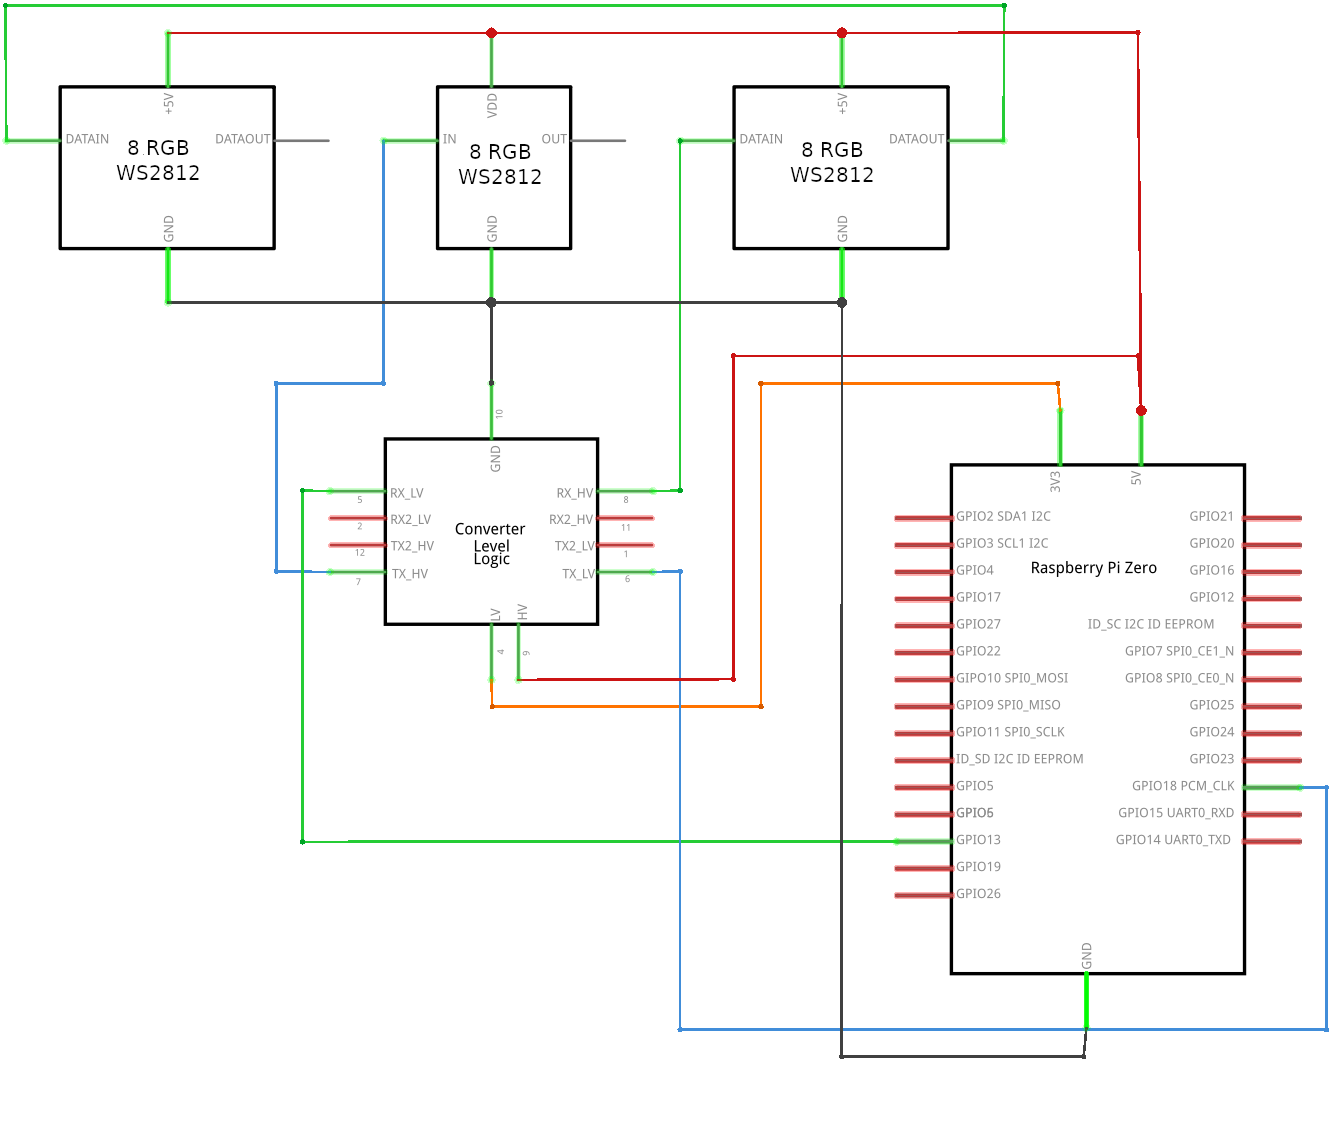
\includegraphics[scale=1]{imaxes/circuito-leds.png}
  \caption{Diagrama de conexión dos leds.}
  \label{fig:conexions_leds}
\end{figure}

\subsection{Software de Control}
Para manexar os leds utilizaremos a libraría rpi\(\_\)ws281x de Jeremy Garff~\cite{garffUserspaceRaspberryPi2019} na sua versión para Python. O seu funcionamento é moi simple, primeiro teremos que configurar os parámetros da tira led, coma o numero de leds, o pin a que esta conectado, o tipo de tira  ou a canle \emph{PWM} entre outros. No programa principal deberemos inicializar os leds con estes parámetros e executala coa función \emph{begin}. Cada vez que queiramos que os les cambien os seu estado chamaremos a función \emph{show}.

Escribiranse funcións encargadas dos padróns de iluminación. Estes padróns serán os seguintes:
\begin{itemize}
    \item \textbf{Luz vermella fixa},
    é a encargada de indicar a posición da bicicleta.
    \item \textbf{Luz vermella intermitente},
    a sua función é a mima que a anterior, pero o padrón de palpadeo aumentara a visibilidade. Crearanse distintos padróns combinando distintas frecuencias en intensidades lumínicas.
    \item \textbf{Luz vermella incremental},
    é a encargada de indicar a freada, a sua intensidade aumentará ata o valor máximo para emular as luces de freada dos coches.
    \item \textbf{Luz amarela de xiro a esquerda ou dereita},
    indica o xiro iluminando progresivamente os leds do anel dende os situados no centro ata os do estremo esquerdo ou dereito, de dispoñer das tiras extra de leds de xiro estas iluminaranse a continuación. Unha vez iluminados tódolos leds estes se apagarán e o padrón repetirase de novo.
\end{itemize}

Tamén se escribirá unha función para controlar a intensidade dos leds en función dun valor numérico recibido, 0 será mínimo e 100 a máxima intensidade.

\section{Cámara}

A cámara a utilizar é a Raspberry Pi Camera, probarase a versión 1 e a versión 2, ambas conectarase a Rasberry Pi Zero co mesmo cable, o conector da placa é delicado polo que deberase conectar con coidado. Para habilitala executarase o comando \emph{raspiconfig} na terminal e no apartado de interfaces activarase a opción cámara.

 Na táboa~\ref{tab:comparativa_camaras} móstrase unha comparativa de ámbalas dúas cámaras e na foto da figura~\ref{fig:camaras} poden verse as tres cámaras a utilizar, a versión 1.3 a versión 2.1 e a 2.1 sen filtro infravermello.
\begin{table}[tb]
    \label{tab:comparativa_camaras}
    \caption{Táboa comparativa da Raspberry Pi Camera V1 e V2~\cite{mocqRaspberryPiPi2017}}
    \begin{center}
        \begin{tabular}{|l|l||l|}
            \hline
              &  V1 & V2\\ \hline
             Sensor  & 5 Mpíxeles & 5 Mpíxeles \\ \hline
             Resolución foto  & 2592x1944 & 3280x2464 \\ \hline
             Vídeo maxi & 1080p & 1080p \\ \hline
             Tamaño do módulo& 20x25x10 mm & 25x23x9 mm \\ \hline
        \end{tabular}
    \end{center}
\end{table}

\begin{figure}[tb]
  \centering
  \includegraphics[scale=.06]{imaxes/camaras.jpg}
  \caption{De esquerda a dereita a Raspberry Pi Camera Module V1, V2 sen filtro infravermello e V2 cunha lente de gran angular}
  \label{fig:camaras}
\end{figure}
\subsection{Lentes}
Para poder capturar o completo da estrada a cámara necesitará de algún tipo de lente que permita un maior campo de visión. Existen versións da cámara que xa inclúen unha lente, pero tamén poderemos atopar lentes externas coma es destinadas para os dispositivos móbiles, que contan co tamaño necesario para a cámara da Raspberry. Na figura~\ref{fig:lentes} móstranse as lentes a probar e analizar as tres superiores colocaranse sobre a cámara e as tres inferiores so para a versión da cámara que incorpora lente.
\begin{figure}[tb]
  \centering
  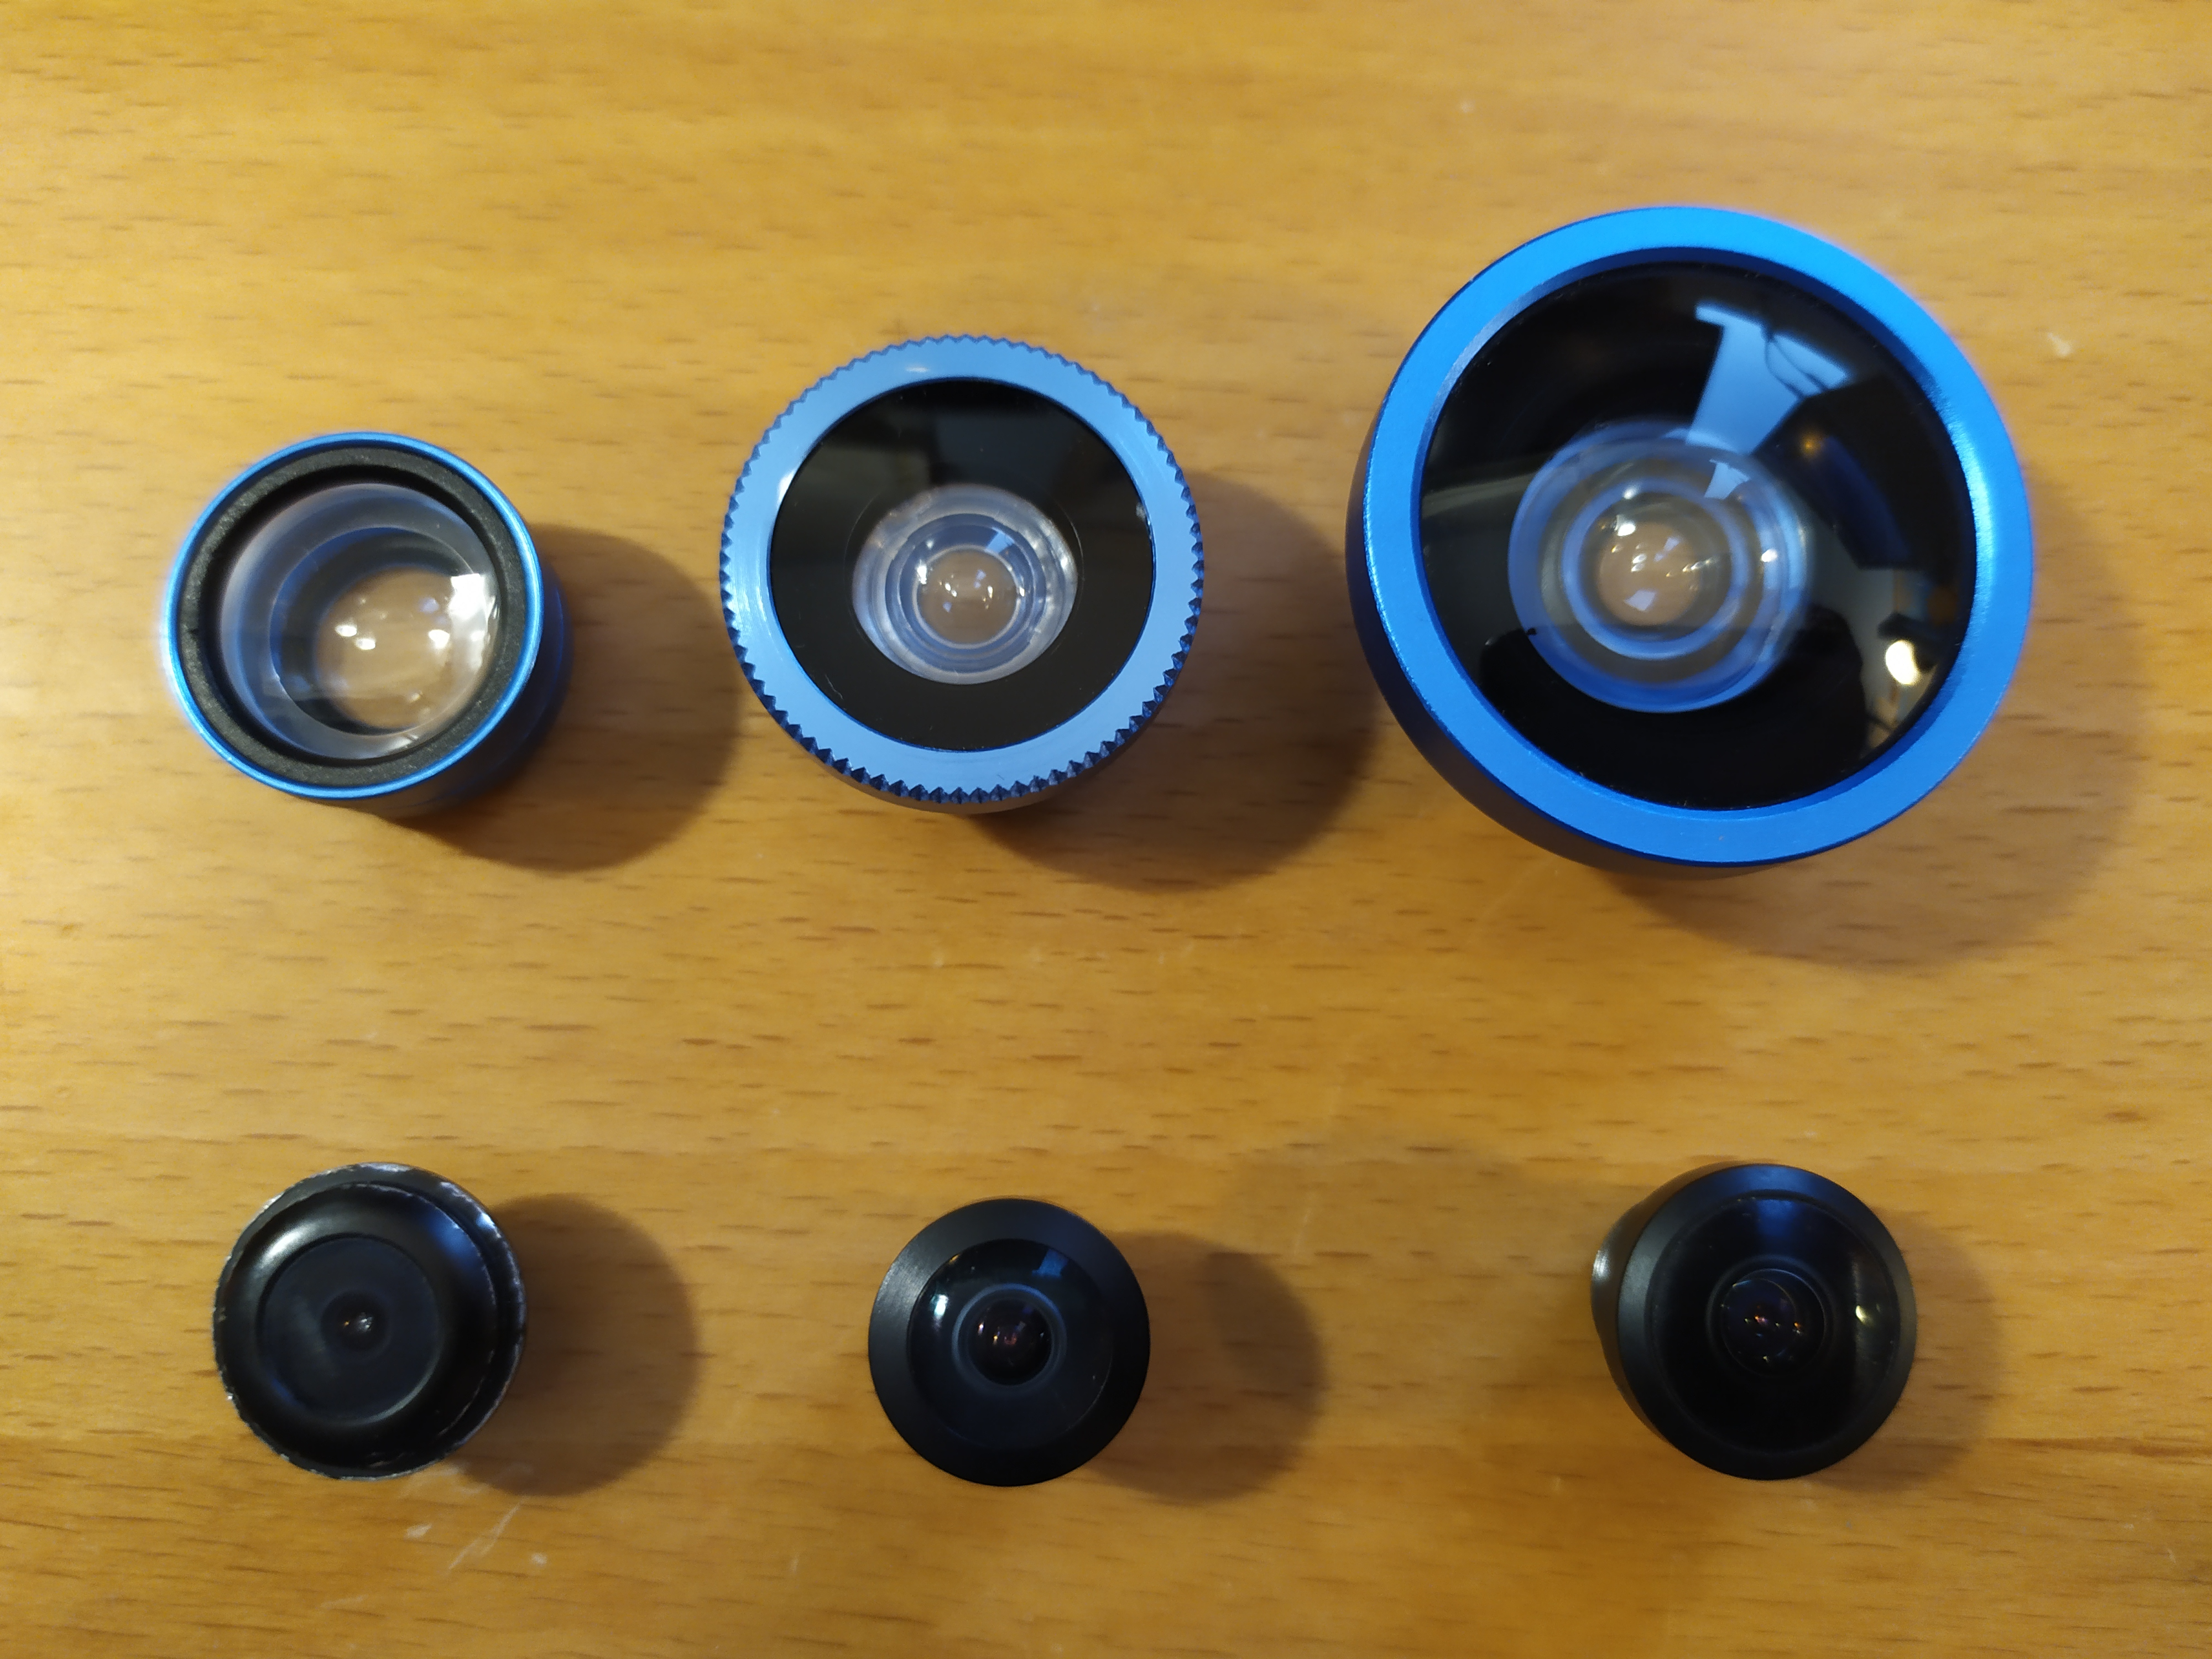
\includegraphics[scale=.06]{imaxes/lentes.jpg}
  \caption{Lentes con diferente ángulo de visión. De esquerda a dereita: fila superior 0.67x, 180º, 0.4x, fila inferior 130º, 160º, 220º }
  \label{fig:lentes}
\end{figure}

\subsection{Captura de vídeo}
\emph{Raspivideo} é o software que utilizaremos para capturar as imaxes, o programa executase dende terminal proporcionándolle diferentes parámetros. No noso caso os parámetros a utilizar serán:
\begin{itemize}
    \item -t Tempo de captura de vídeo, no noso caso será 0 indicando que a captura será continua.
    \item -w e -h Son os parámetros de anchura e altura de píxeles, probaremos diferentes resolucións para conseguir a máxima calidade posible sempre que o tamaño da imaxe non repercuta na latencia de transmisión.
    \item -fps \emph{Frames per second}, é o numero de imaxes a capturar cada segundo, variaremos con este valor para minimizar a latencia.
    \item -b \emph{Bitrate}, o numero de bits por segundo, buscaremos o valor máis alto posible sen que produza retardos na transmisión.
    \item -n Con este parámetro deshabilitaremos a previsualización do vídeo.
    \item -pf Parámetro para elixir o perfil do codificador de vídeo H264, as opcións dispoñibles son, \emph{baseline}, \emph{main} and \emph{high}. Utilizaremos a opción \emph{baseline} xa que é a que menor custo computacional ten.
    \item -o Con este parámetro indicamos a saída de vídeo, como por exemplo a un arquivo, no noso caso utilizaremos a saída estándar que indicaremos con "-" , e que redirecionaremos máis tarde.
\end{itemize}

\section{Transmisión de vídeo}
Para transmitir o vídeo ao dispositivo móbil a través da rede preséntanse varias posibilidades. Para comparalas transmitiremos vídeo dende a Raspberry Pi cunha mesma resolución, 720p, e recibiremos e reproduciremos o nun pc mediante \emph{vlc}.

\begin{itemize}
    \item A primeira opción a analizar é o software de vídeo \emph{vlc}, unha completa ferramenta de reprodución que tamén permite a transmisión e e a recepción de vídeo na rede mediante diferentes protocolos. Faremos unha proba utilizando o \emph{vlc} na Raspberry Pi para transmitir o vídeo da cámara e recibilo nun pc con \emph{vlc}. Como resultado obtemos unha transmisión cunha latencia superior a un segundo, que imposibilita o seu uso para controlar o trafico en tempo real.

    \item A segunda opción que probaremos consistirá en capturar o vídeo coa ferramenta de captura de vídeo da Raspberry Pi, \emph{raspivid}, e redirecionar a sua saída a rede utilizando \emph{netcat} unha utilidade para transmitir e recibir na rede mediante \emph{tcp} ou \emph{udp}. Transmitiremos mediante \emph{udp} para conseguir unha menor latencia a custo de perder algún fotograma. A recepción de vídeo a realizaremos nun pc mediante \emph{vlc} coma no caso anterior. A latencia obtida neste caso e mellor que no anterior.

    \item Buscando reducir aínda máis a latencia probaremos a utilizar o software \emph{socat}, que funciona de forma similar a \emph{netcat} e conta tamén con moitas opcións de configuración. O procedemento será igual que no caso anterior, faremos a captura con \emph{raspivid} e redirecionaremos o vídeo a un porto nunha dirección \emph{ip} mediante \emph{udp} neste caso utilizando \emph{socat}. Como resultado obtemos unha latencia aínda menor que con \emph{netcat} polo que utilizaremos este software para a transmisión de vídeo.
\end{itemize}

\section{Recepción de ordes}

 Para recibir os comandos enviados dende o dispositivo móbil e executalos mediante Python implementaremos un servidor tamén Python para poder integrar a recepción e a execución de ordes no mesmo programa.

 A primeira opción será utilizar peticións \emph{http} e manexalas mediante a clase de Python \emph{BaseHTTPRequestHandler}, o problema é que esta clase bloquea o programa mentres se executan as ordes correspondentes a petición recibida. Para solucionar este problema poderiáse implementar un servidor \emph{multithread} ou utilizar unha libraría para Python que implemente o servidor \emph{multithread} de forma transparente. Plantexase utilizar as librarias \emph{multithread} \emph{Tornado}, \emph{Twisted} ou \emph{lighttpd} pero debido os recursos limitados da Rasberry Pi Zero o uso dunha destas librarías podería implicar maiores latencias e consumo enerxético.

 Finalmente optase por manexar a conexión directamente mediante \emph{sockets} non bloqueastes é así poder utilizar un solo \emph{thread}. Para elo introduciremos as peticións de conexión nunha lista, unha vez aceptada introducirase nunha segunda lista as mensaxes recibidas e se executara a orde correspondente para cada mensaxe.

As mensaxes serán as seguintes:
\begin{itemize}
    \item \textbf{r} para o xiro a dereita.
    \item \textbf{l} para o xiro a esquerda.
    \item \textbf{n} para a luz de noite.
    \item \textbf{b} para a luz de freo.
    \item \textbf{k} para o padrón de palpadeo.
    \item \textbf{o} para apagar as luces.
    \item \textbf{v} para iniciar a captura e transmisión de vídeo.
    \item \textbf{vs} para deter a captura e a transmisión de vídeo.
    \item \textbf{c} para comprobar que a conexión segue aberta.
    \item \textbf{valor numérico} para establecer a intensidade das luces.
\end{itemize}

\section{Conexión co servidor}
Os dispositivos conectaranse mediante unha rede local, xa sexa a través dun cable usb ou dunha rede wi-fi, en ámbolos dous casos o dispositivo Android será o encargado de aloxar a rede xa sexa compartindo por usb ou creando un punto de aceso wi-fi.

Para permitir que o dispositivo móbil se conecte o servidor sen ter que coñecer a dirección \emph{ip} de este procederase da seguinte maneira. Dende o servidor crearase un \emph{thread} no que se abrira un \emph{socket} encargado de enviar unha mensaxe a dirección de \emph{broadcast} para que poda ser recibido por tódolos dispositivos da rede.

\section{Autoarranque do servidor}
O servidor deberá arrancar automaticamente o acender o dispositivo, e arrancar de novo se por algún motivo detense a súa execución. Para elo crearemos un servizo en \emph{sytemd} que se encargará de arrancar o programa e reinicialo se é necesario. A estrutura do servizo e a seguinte, indica a localización do programa Python a executar, a orde de reiniciar sempre, os \emph{logs} a utilizar para rexistrar as execucións e os fallos, e o usuario e grupo que o executará. Situaremos o ficheiro do servizo na ruta \textit{/etc/systemd/system/} e unha vez ali o habilitaremos coa orde \textit{sudo systemctl enable bikeview.service} agora o servizo executarase cando se arranque o dispositivo e reiniciarase se se para.

\section{Alimentación e enerxía}
O consumo de amperios da Raspberry Pi Zero sen carga de traballo é duns 120 mA, gravando vídeo a 1080p o consumo é de 230mA, gravarase vídeo a 720p polo que o consumo será algo menor pero engadirase o consumo do chip wifi funcionando. Os leds ws2812 teñen un consumo máximo de 60 mA cada un 20 mA como máximo por cada un dos tres leds \emph{RGB} a máxima intensidade, o noso máximo consumo realizarse coa luz vermella acesa de forma continua, xa que no resto de modos os padróns de palpadeo reducen o consumo. Contamos con 24 destes leds polo que o consumo máximo será de 20mA por 24 leds, un total de 480mA que sumados o consumo da Raspberry Pi nos da un consumo máximo teórico de 710mA na versión sen leds intermitentes o consumo seria de 160mA máis 230mA, en total 390mA.

\begin{itemize}
    \item Unha primeira versión máis sinxela contará solo cunha batería usb para alimentar a Raspberry. Os requisitos de esta batería serán a amperaxe e a capacidade.

    Partirase do valor do consumo máximo aproximado de 400mA para calcular o tempo de funcionamento. Con esta amperaxe aos 5V que funcionan a Raspberry e os leds a potencia utilizada sería de 2W. Neste suposto unha batería de  5000mAh cunha voltaxe nominal de 3.7V pode proporcionar 18.5Wh polo que duraría ata 9 horas e 15 minutos, no caso dunha batería de 1000mAh o tempo mínimo teórico de funcionamento sería de algo menos de dúas horas.
    Comprobaremos se estes supostos se cumpren facendo medicións do tempo de funcionamento.

    \item Realizaremos unha segunda versión máis avanzada que apagará o dispositivo cando a batería baixe de certo limite de voltaxe para evitar que o dispositivo se desconecte e contará tamén cun pulsador para poder acendela e apagala.

    Para isto utilizaremos o chip de carga Adafruit Powerboost 1000 que conta cunhas características moi interesantes a maiores da protección de sobrecarga conta cunha led e un pin que se activaran cando a voltaxe da batería baixe dos 3.2v, unha voltaxe operacional de 5.2v para evitar perdidas de voltaxe en cables e conectores, un pin habilitador que permite conectar ou desconectar a batería, e proporciona 1 amperio de intensidade sen baixar a voltaxe dos 5v. Non conta con protección de sobrecarga polo que as batería que utilicemos deben incluír un circuíto de protección, este é o caso da maioría de baterías, de utilizar unha sin protección, como unha cela 18650, deberemos engadir o circuíto de protección ou asegurarnos de implementar o apagado por voltaxe baixa correctamente.

    A realización o circuíto basearase no guía \emph{lipopi} de Daniel Bull~\cite{bullGuideSettingLiPo2019} que utiliza o Adafruit Powerboost, nas súas dúas versións a de 500 mA e 1 A, para programar o apagado automático da Rapberry Pi cando a batería baixe de 3.2v e un pulsador para o acendido, tamén conta con dúas versións máis unha que tamén permite o apagado, e outra que monitoriza a voltaxe da batería. Realizarase a versión con pulsador para acendido e apagado.

    O funcionamento é o seguinte, o premer o pulsador conéctase o positivo da batería co pin abilitador, acendendo o adafruit powerboost e por conseguinte acendendo a Raspberry Pi. O acender a Raspberry Pi un pin conectado o pin habilitador acenderase pare seguir mantendo un valor positivo. Para evitar que o voltaxe no pin habilitador caia no tempo entre que pulsamos o pulsador e a Raspberry Pi arranca e encárgase de manter o valor positivo, situaremos un circuíto RC formado por un condensador cunha resistencia en paralelo entre o pulsador e o pin habilitador. O condensador cargarase cando o pulsador cerre o circuíto e descargarase a continuación mantendo a voltaxe o tempo suficiente para que a Raspberry arranque e acenda o pin. Utilizarase un condensador de 100\(\mu\)F xunto cunha resistencia 100k\(\Omega\) que proporcionan un tempo suficiente de 10 segundos. O pin da Raspberry que utilizaremos para este propósito pode ser o 14 correspondente a conexión \emph{uart}, que se acenderá coa Raspberry e se desconectará cando se apague, engadiremos unha resistencia de 10k\(\Omega\) para protexer este pin. Tamén poderíase utilizar calquera outro pin de propósito xeral indicando no arquivo de configuración \emph{config.txt} na partición \emph{boot} da Raspberry, que o pin arranque cun valor positivo e cun valor negativo cando o dispositivo se apague, no caso de utilizar o pin \emph{GPIO} 5 as ordes serían as seguintes: \emph{$gpio=5=op,dh$} para que o pin arranque con valor positivo, \emph{$dtoverlay=gpio-poweroff,gpiopin=5,active_low="y"$} para deixar o pin apagado cando se apaga a Raspberry.

    Para o apagado utilizarase un segundo pin conectado o pulsador, cando este se pulse, estando a Rasberry acesa, se conectará a voltaxe da batería, cando este valor positivo chegue o pin un script Python encargarase de apagar o dispositivo. Engadiranse un divisor de voltaxe para reducir a voltaxe da batería xa que cando está completamente cargada a sua voltaxe de 4.2v e superior o máximo valor lóxico tolerado pola Raspberry Pi de 3.3V. Utilizaremos unha resistencia de 33k\(\Omega\) conectada entre o pin e a batería e unha resistencia de 100k\(\Omega\) entre o pin e terra. Para evitar que o pin de acendido dispare o apagado situarase un díodo entre o pin de acendido e apagado evitando que a voltaxe circule nesa dirección.

    Finalmente conectarase o pin indicador de batería baixa a outro pin de entrada da Raspberry que mediante o script Python apagará o dispositivo. O diagrama de funcionamento mostrase na figura~\ref{fig:circuito_alimentacion}.

    \begin{figure}[tb]
      \centering
    	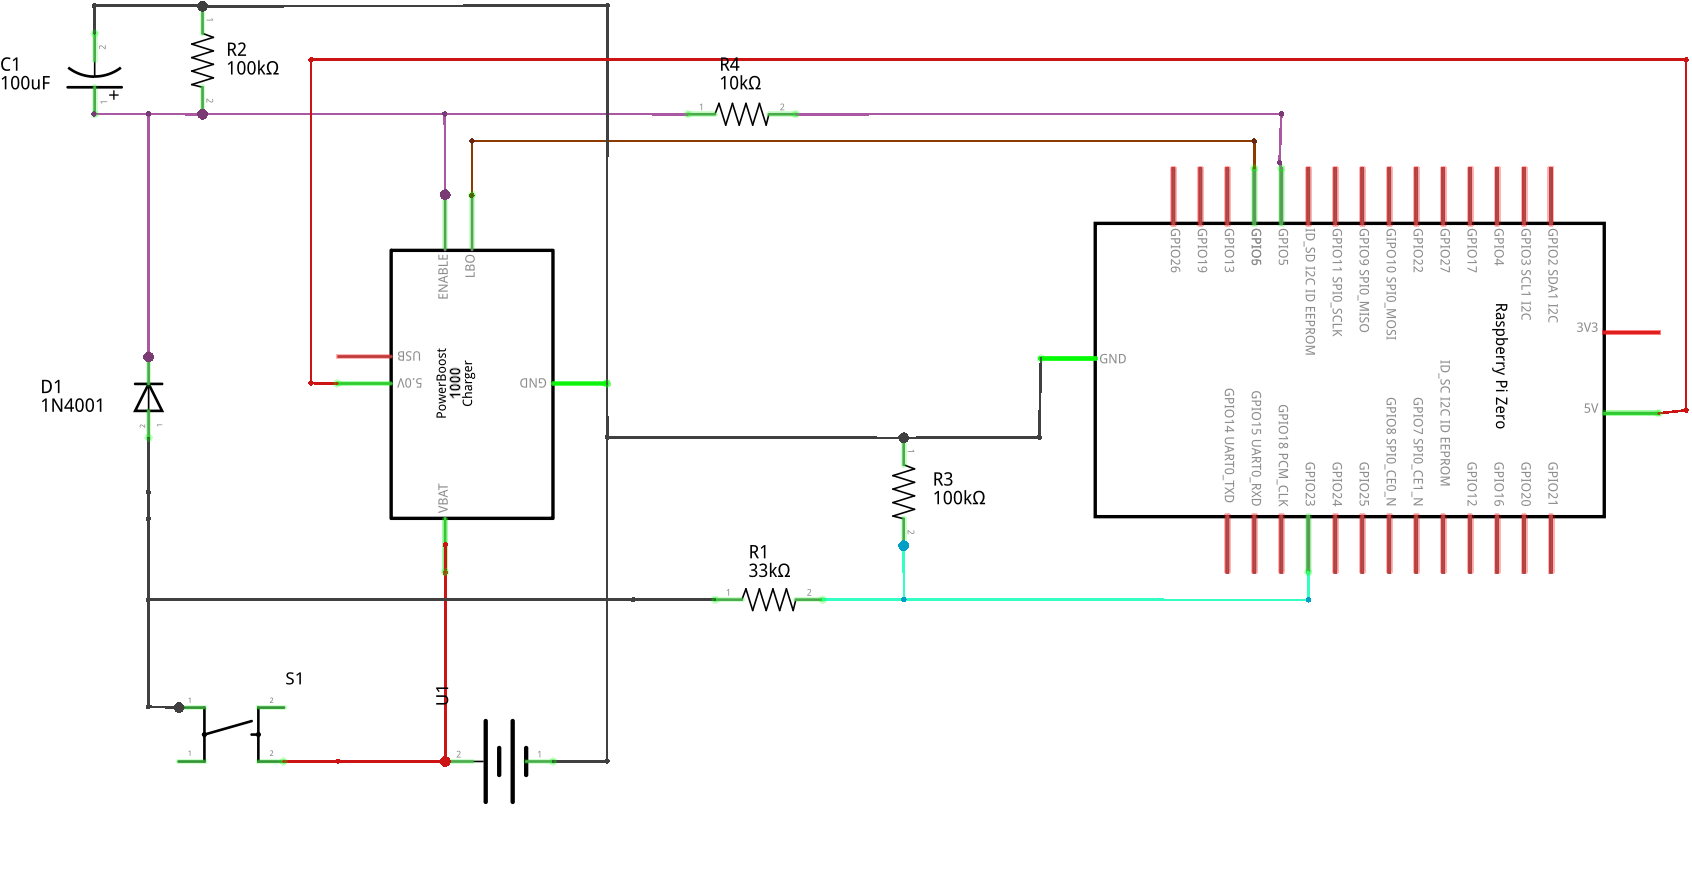
\includegraphics[scale=1]{imaxes/circuito-bateria.png}
    	\caption{Diagrama de funcionamento do circuíto de alimentación.}
    	\label{fig:circuito_alimentacion}
    \end{figure}

    Na figura~\ref{fig:circuito_dispositivo} podemos ver o diagrama final do dispositivo e na figura~\ref{fig:esquema_dispositivo} o esquema completo integrando os leds o circuíto de carga e a cámara.

    \begin{figure}[tb]
      \centering
    	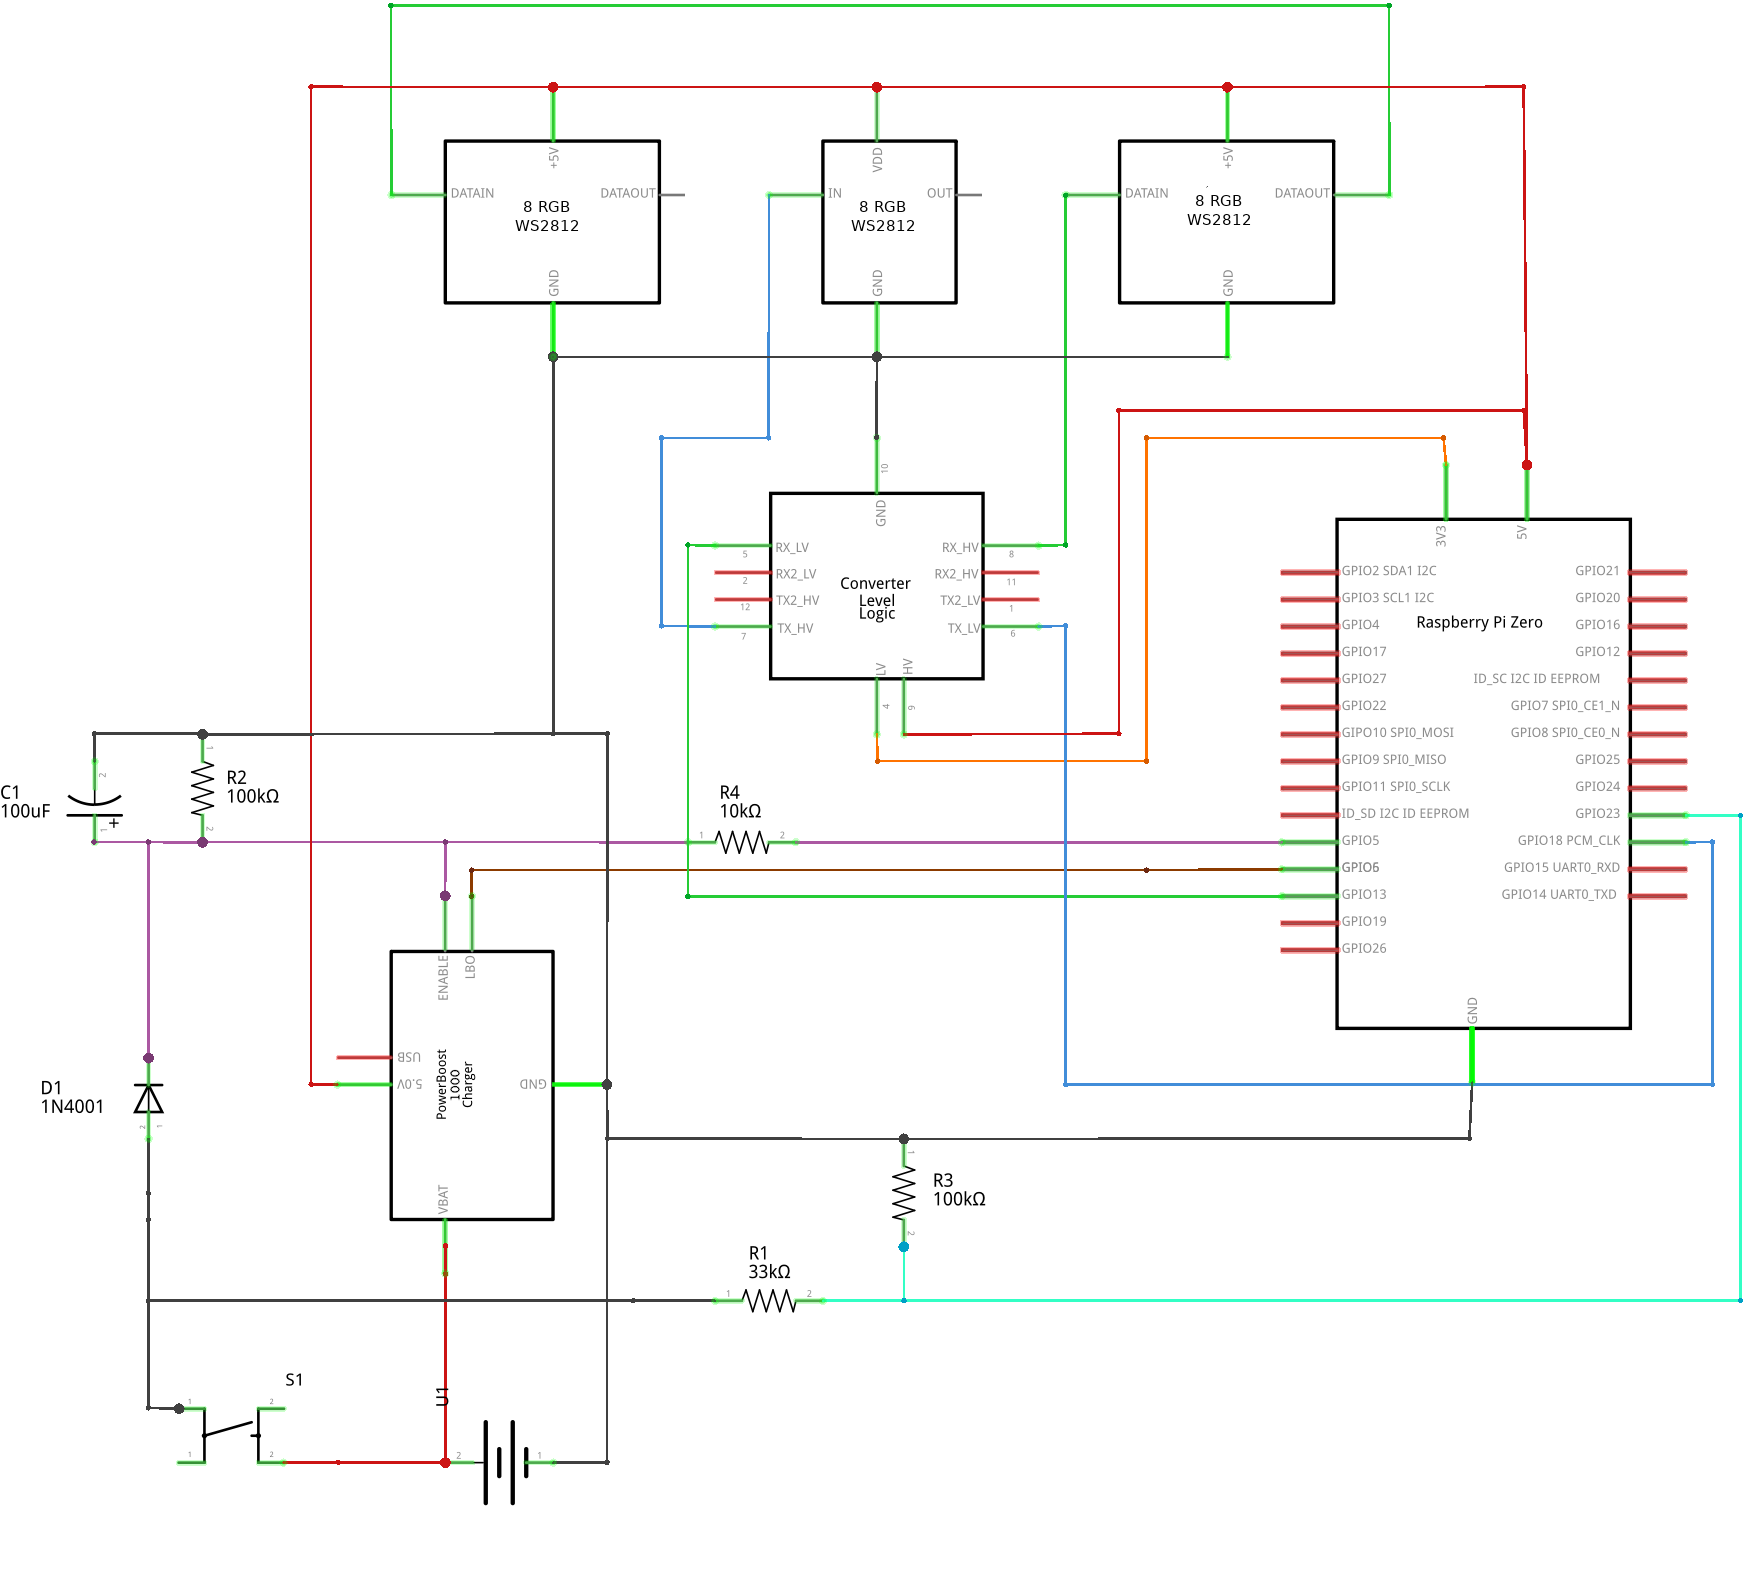
\includegraphics[scale=1]{imaxes/circuito-completo.png}
    	\caption{Diagrama do dispositivo.}
    	\label{fig:circuito_dispositivo}
    \end{figure}

    \begin{sidewaysfigure}[tb]
      \centering
    	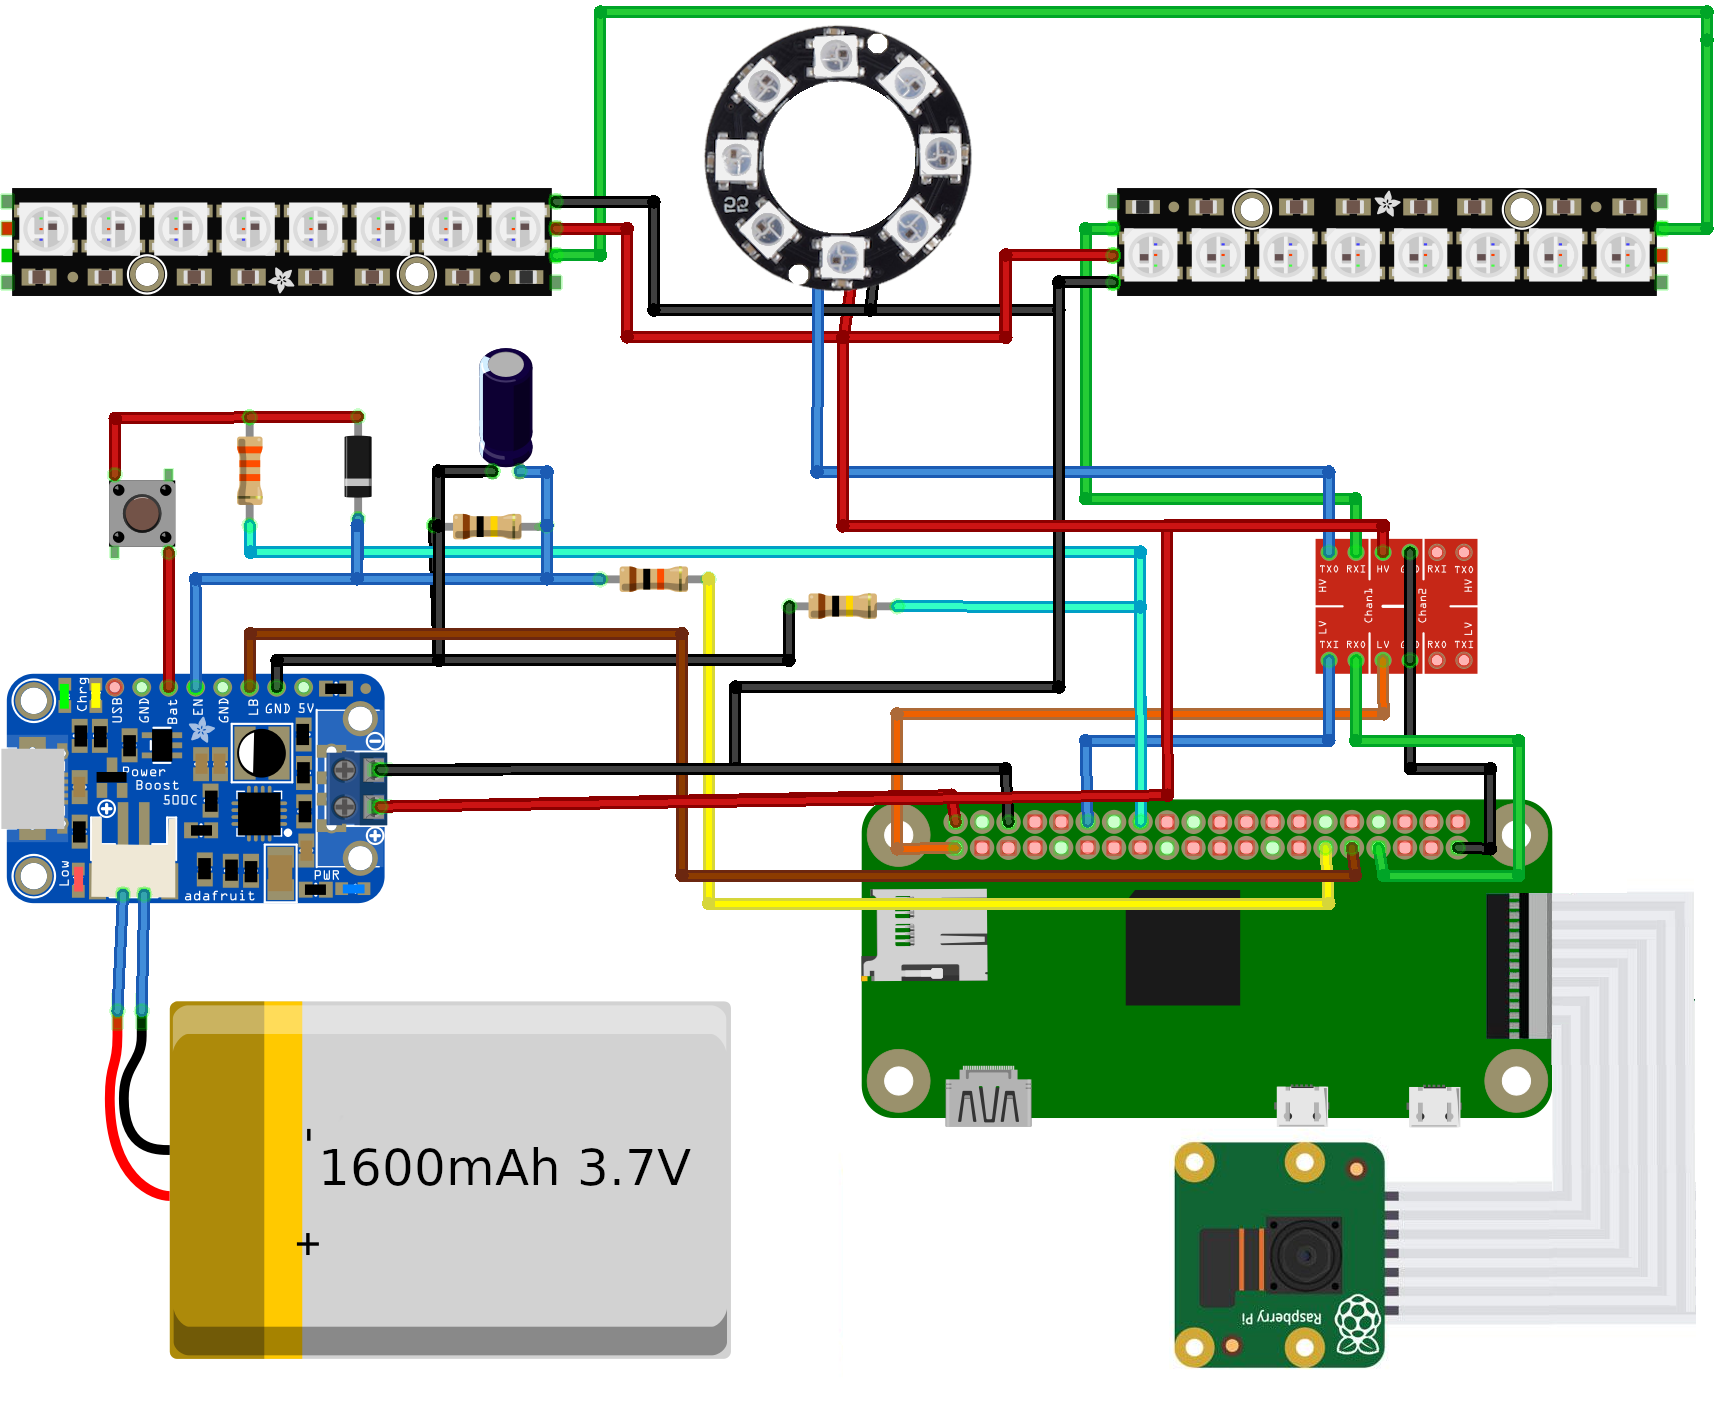
\includegraphics[scale=1]{imaxes/esquema-completo.png}
    	\caption{Esquema completo do dispositivo.}
    	\label{fig:esquema_dispositivo}
    \end{sidewaysfigure}

    Para arrancar automaticamente o script Python instalarase un novo servizo en \emph{sytemd} e de igual maneira que co servidor executarase no arranque e cada vez que se pare.

    Na implementación física colocaremos o chip de carga xunto cos compoñentes electrónicos nunha placa cun conector para poder conectalo directamente os conectores da Raspberry Pi Zero. Tamén colocarase nesta placa o conversor lóxico de nivel como se ve na figura~\ref{fig:fotos_reverso}

    \begin{figure}[tb]
      \centering
    	\includegraphics[scale=.05]{imaxes/foto-circuito1.jpg}
    	\includegraphics[scale=.05]{imaxes/foto-circuito2.jpg}
    	\caption{Imaxes do circuíto por ambas caras.}
    	\label{fig:fotos_reverso}
    \end{figure}

    Na elección da batería teremos en conta a maiores da sua capacidade o seu tamaño e forma, sendo o ideal que sexa similar o da Raspberry para poder integrala no dispositivo con facilidade. Por eso elixiremos unha batería de 1600mA e 5.92Wh con circuíto de protección e unhas dimensións de 9 x 34 x 50mm que para este suposto, xa que engadindo os leds extra calcúlase un consumo máximo de 3.55W, debería proporcionar un tempo mínimo de funcionamento de 2 horas aproximadamente.

\end{itemize}

\section{Carcasa e ancoraxe}

Para protexer o dispositivo e suxeitalo baixo a sela da bicicleta plantexaranse dúas opcións.
\begin{itemize}
    \item A primeira realizarase para a versión do proxecto alimentada cunha batería usb. Consistirá en utilizar a carcasa oficial da Raspberry Pi Zero que inclúe un oco para a cámara e espazo para as conexión na parte de atrás, a carcasa so permite a uso de cámaras sen lentes polo que incorporarase unha lente externa.

    Para suxeitar a carcasa a bicicleta deseñaremos un soporte en 3d co software Blender. Partiremos das medición da carcasa e deseñarase un soporte que suxeite a carcasa firmemente e permita atala a barra da sela mediante unha correa.

    Unha vez deseñado e tras comprobar que o deseño e imprimible exportarase no formato \emph{STL} que abrirase cun software encargado de dividir o deseño en capas e traducilo a ordes de desprazamento interpretables pola impresora, aquí configuraranse diferentes parámetros como a altura de capa, que é a resolución de impresión, as velocidades, a cantidade e tipo de recheo da peza ou o uso de soportes para facilitar a impresión. Neste caso utilizaras o software libre Slic3r no que configurarase a peza a imprimir cun 100\(\%\) de recheo para que sexa máis sólida cunha altura de capa de 0.2mm e sen uso de soportes, como resultado obterase un arquivo \emph{GCODE}  que pasaremos a impresora. O prototipo imprimirase o prototipo en 3d probarase e aplicaranse correccións no modelo. Para este deseño realizáronse dúas iteracións móstranse na figura~\ref{fig:soporte_caixa}.

    \begin{figure}[tb]
      \centering
      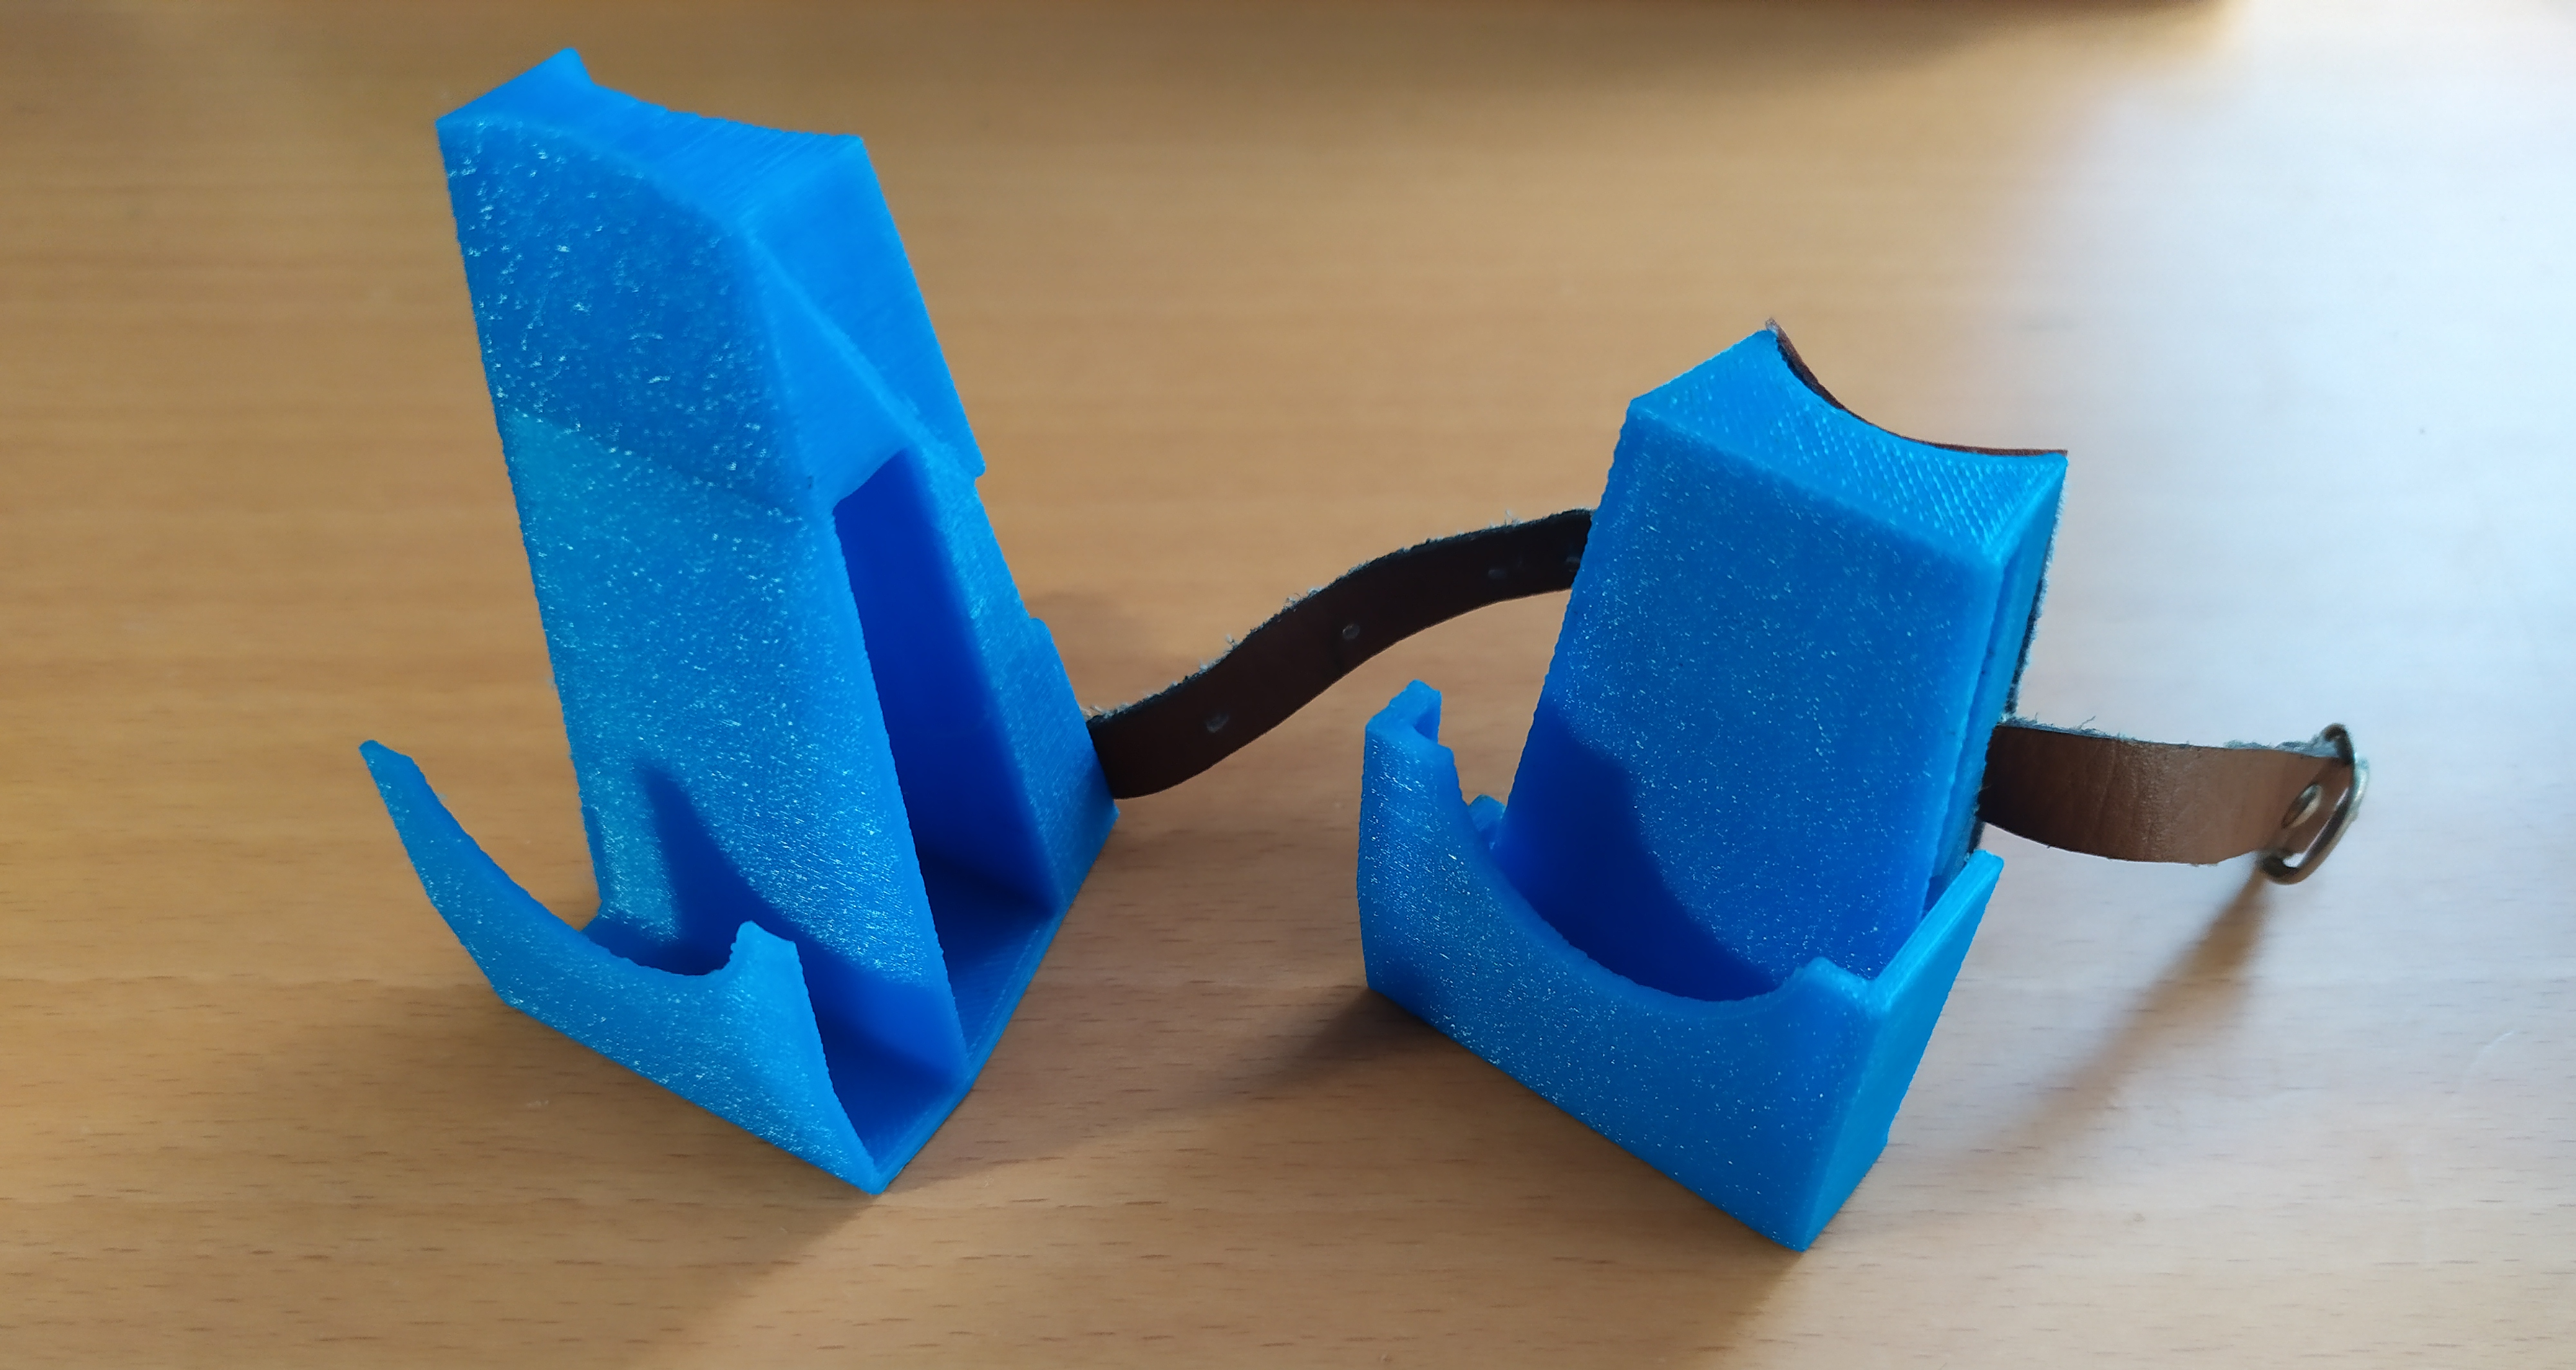
\includegraphics[scale=.1]{imaxes/soporte-caixa.jpg}
      \caption{Deseños do soporte na bicicleta para a caixa oficia da Rasberry Pi.}
      \label{fig:soporte_caixa}
    \end{figure}


    \item A segunda versión terá que albergar a Raspberry Pi Zero xunto coa cámara, o chip de carga e alimentación, o conversor lóxico de voltaxe e a batería. Utilizaremos tamén neste caso o software de edición 3d Blender para deseñar os prototipos.

    O deseño contara co anel led situado no exterior o redor da lente da cámara, no interior colocaranse tódolos compoñentes electrónicas e a batería. Na parte superior contará cun oco para o conector micro usb de carga e aceso a tarxeta micro sd da Raspberry Pi. No exterior contará tamén con dous brazos articulados nos que situaremos as dúas tiras leds para indicar o xiro.

    Da mesma forma que no caso anterior o deseño imprimirase modificarase e volverase a imprimir ata que se obteña un resultado aceptable. Na figura~\ref{fig:evolucion_carcasa} pódese observar a evolución dos diferentes deseños e na figura~\ref{fig:carcasa} unha imaxe renderizada do deseño final.


    \begin{figure}[tb]
      \centering
      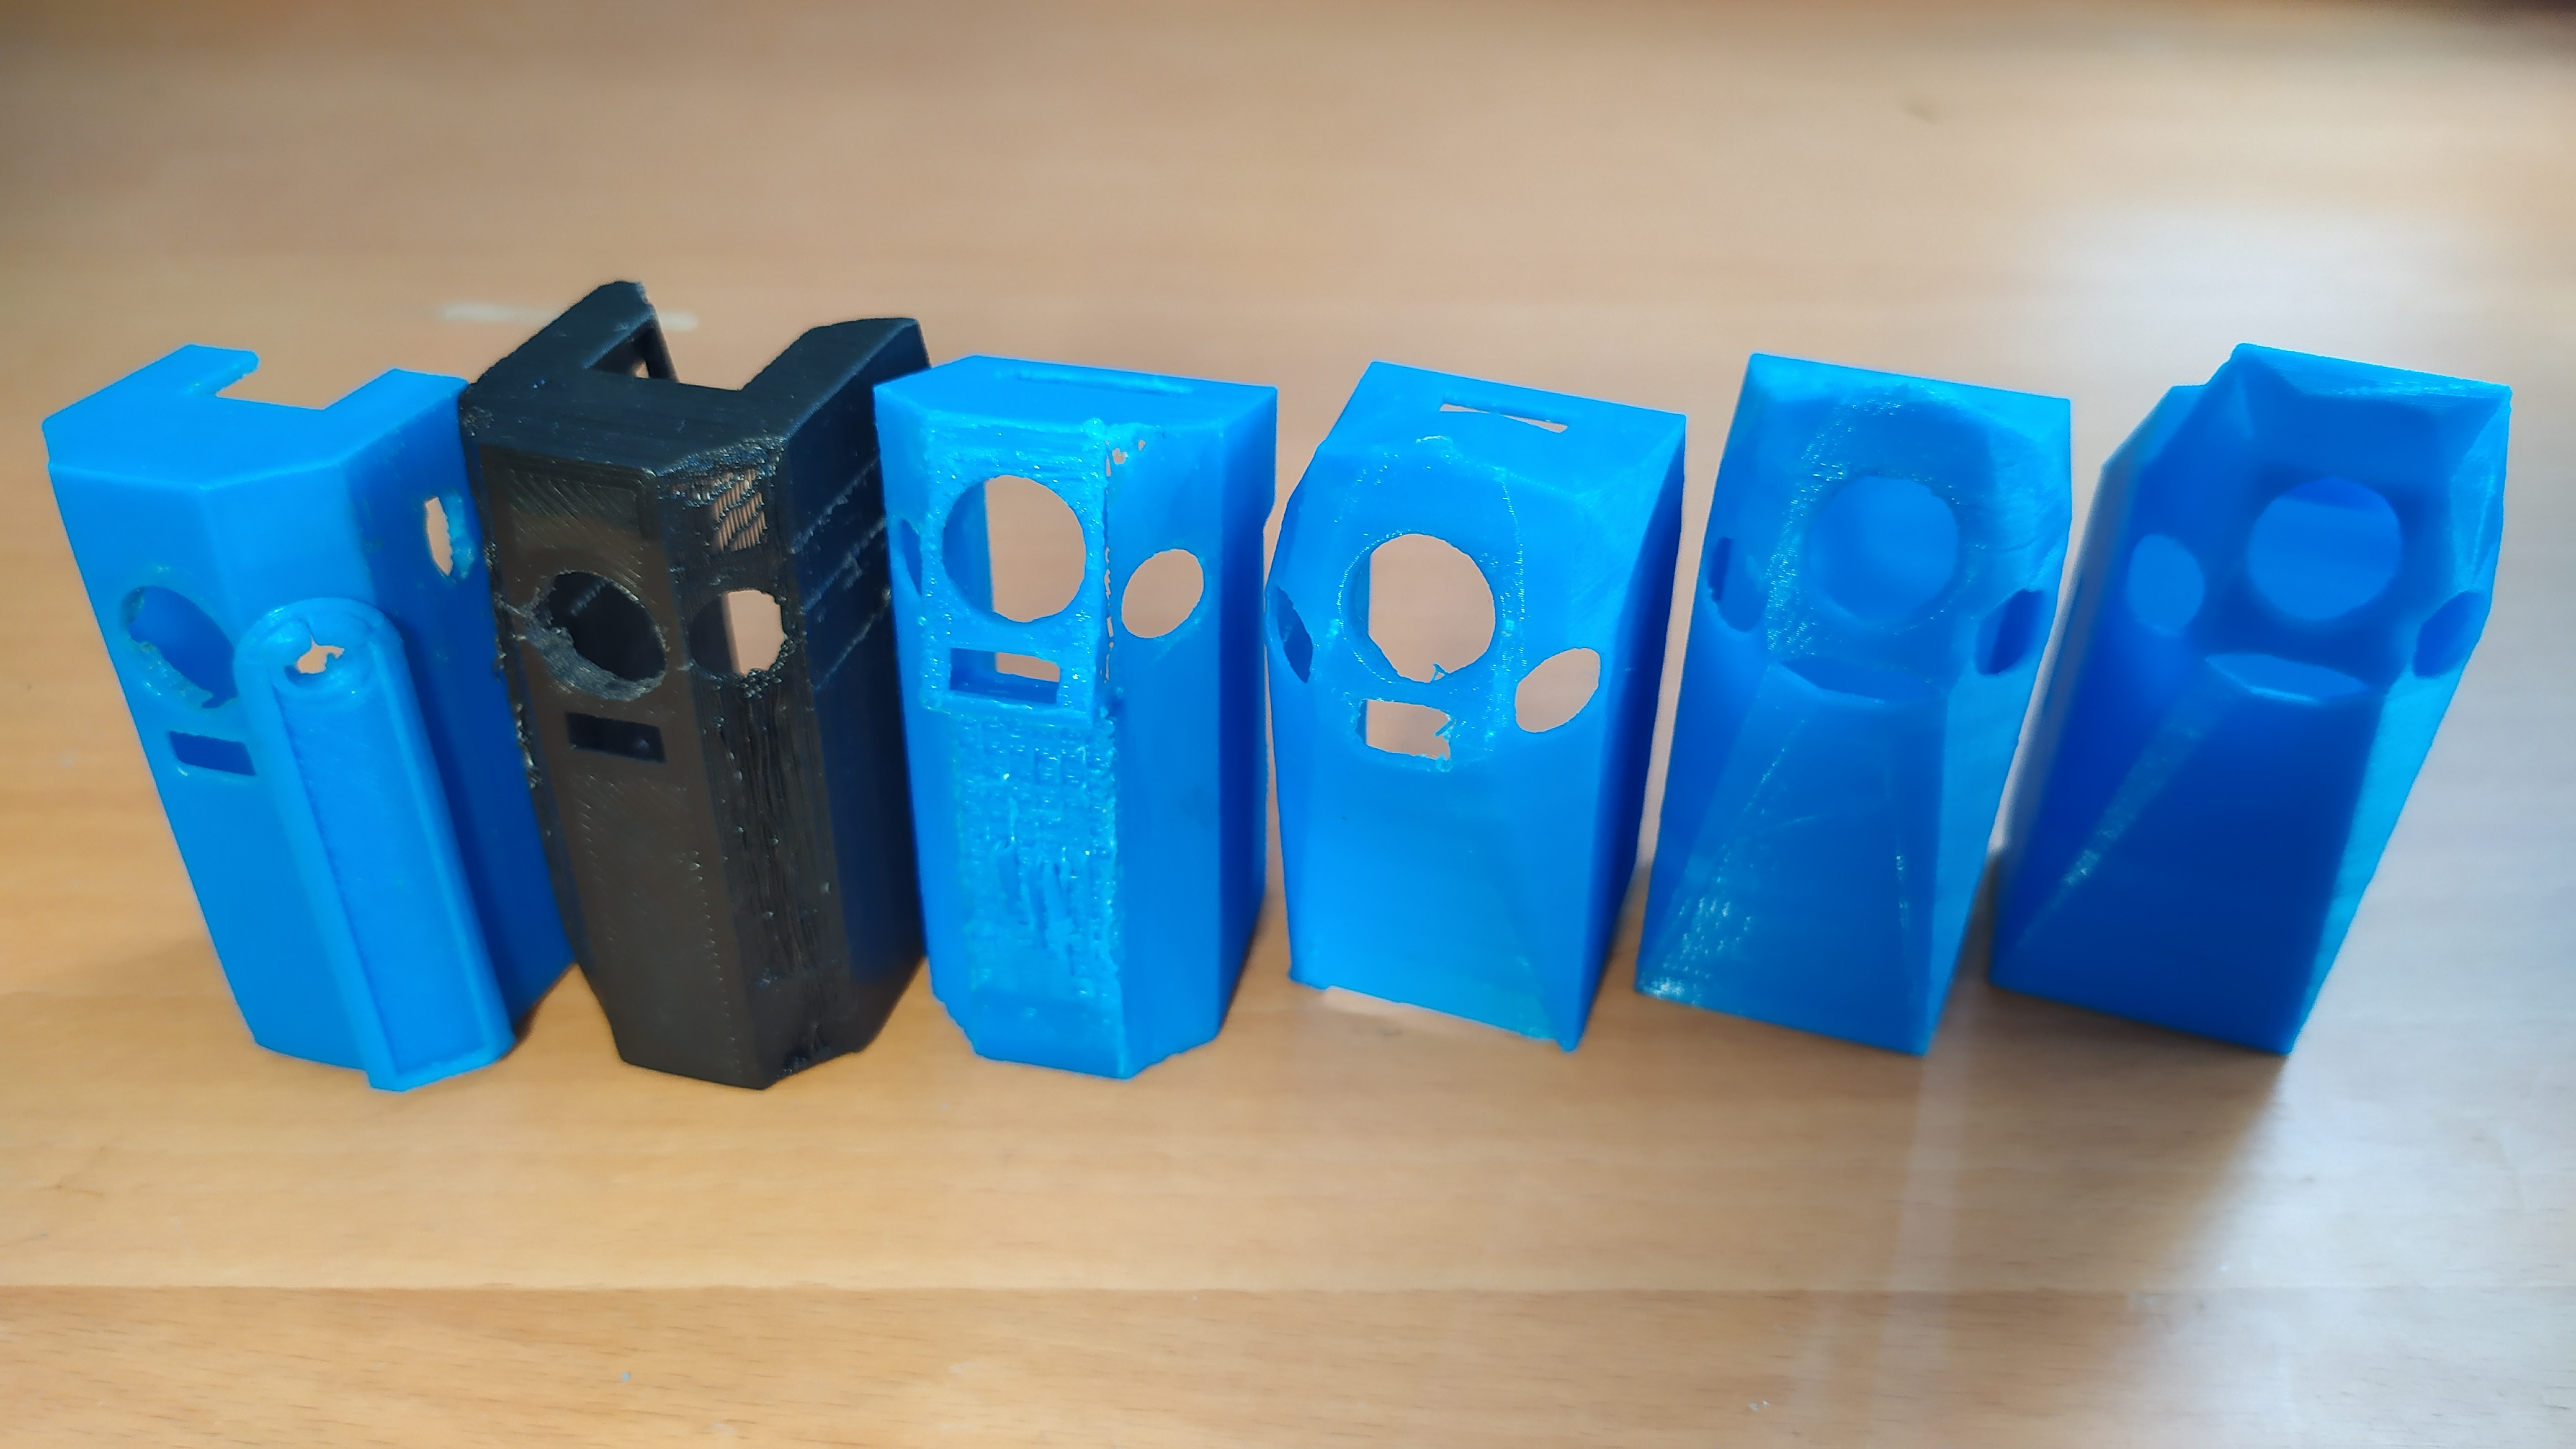
\includegraphics[scale=.1]{imaxes/evolucion-carcasa.jpg}
      \caption{Evolución dos deseños da carcasa.}
      \label{fig:evolucion_carcasa}
    \end{figure}

    \begin{figure}[tb]
      \centering
      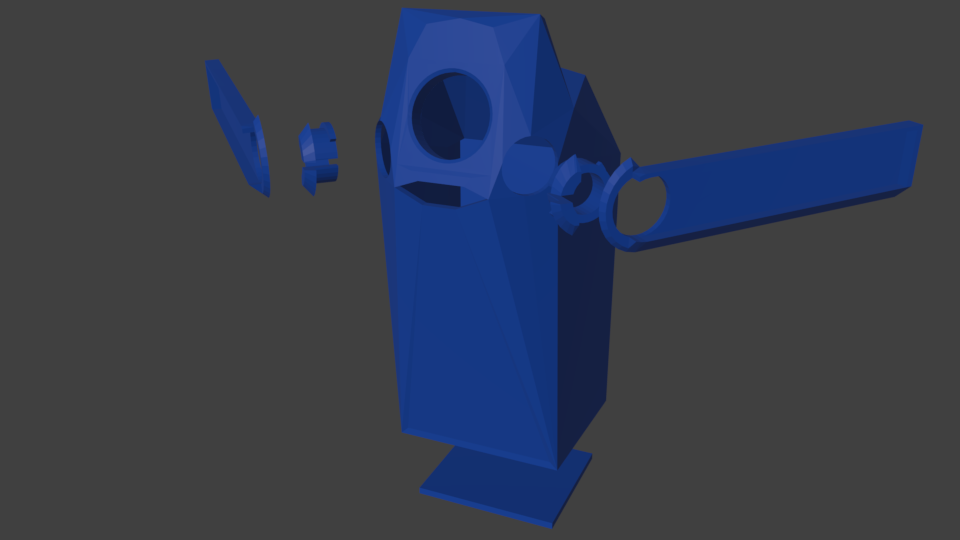
\includegraphics[scale=.4]{imaxes/carcasa.png}
      \caption{Ultimo deseño da carcasa.}
      \label{fig:carcasa}
    \end{figure}
\end{itemize}

 \chapter{Deseño e implementación de BikeView}
\label{chap:implementacion_aplicacion}
\lettrine{P}{artindo} dos requisitos de BikeView elixirase a arquitectura a utilizar e implementarase o software necesario.



\section{Esquema xeral da aplicación}
Para crear esta aplicación Android optarase por utilizar a linguaxe de programación Kotlin e o entorno de programación Android Studio. Kotlin é unha linguaxe de programación creada por JetBrains executable na maquina virtual de Java, dende 2017 Kotlin é unha linguaxe oficial para desenvolver aplicacións Android.

Como mosta o libro Kotlin for Android Developers~\cite{leivaKotlinAndroidDevelopers2018} algunhas das súas vantaxes fronte a Java son:
\begin{itemize}
    \item Unha maior expresividade: Podes escribir máis con menos código.
    \item Maior seguridade: En Kotlin e obrigatorio especificar a nulabilidade dos obxectos e esta se comproba en tempo de compilación.
    \item É funcional: Kotlin é unha linguaxe orientada a obxectos pero inclúe conceptos da programación funcional como as expresións lambda.
    \item Fai uso de extensión de funcións: Permite estender clases con novas funcionalidades se necesidade de ter aceso o código da clase.
    \item É altamente interoperable: Pódese utilizar librerías e clases de Java no mesmo proxecto.
\end{itemize}


A aplicación contará con catro compoñentes. O principal será a \emph{MainActivity}, a encargada de iniciar as compoñentes a visualizar na pantalla, executar as ordes e mostrar a información. O segundo será o \emph{layout} onde se definiran as compoñentes a visualizar e a sua posición en pantalla. O terceiro a clase \emph{request} a encargada da conexión co servidor e de transmitirlle as ordes. O cuarto elemento é a clase encargada de recibir o vídeo e descodificalo.

\section{Actividade principal}
A actividade principal ou \emph{MainActivity} dunha aplicación Android é a primeira pantalla que aparece cando executase a aplicación e a encargada de controlar o seu funcionamento e a sua interface de usuario. Neste caso a actividade será a encargada de mostrar os botóns e encargarse do seu funcionamento, amosar o estado da conexión, encargarse da xestión do sensores e reproducir o vídeo. O mesmo tempo encargarase de instanciar e comunicarse coas clases encargadas da conexión co dispositivo e da recepción de vídeo.

\subsection{Layout}
Un \emph{layout} é a definición da estrutura da interface de usuario. Esta actividade contará con dous \emph{layouts} un para a posición vertical e outro para a posición horizontal da pantalla
\subsubsection{Layout vertical}
Este \emph{layout}, figura~\ref{fig:layout_horizontal}, contará cunha superficie reservada para o vídeo na metade superior da pantalla. Na metade inferior situaranse os botóns encargados de executar as ordes. Na parte superior situase a barra de estado que na sua parte dereita contará cun botón para conectar que servirá o tempo de indicador de conexión, a súa esquerda mostrarase unha barra para controlar a intensidade dos leds.
\begin{figure}[tb]
  \centering
  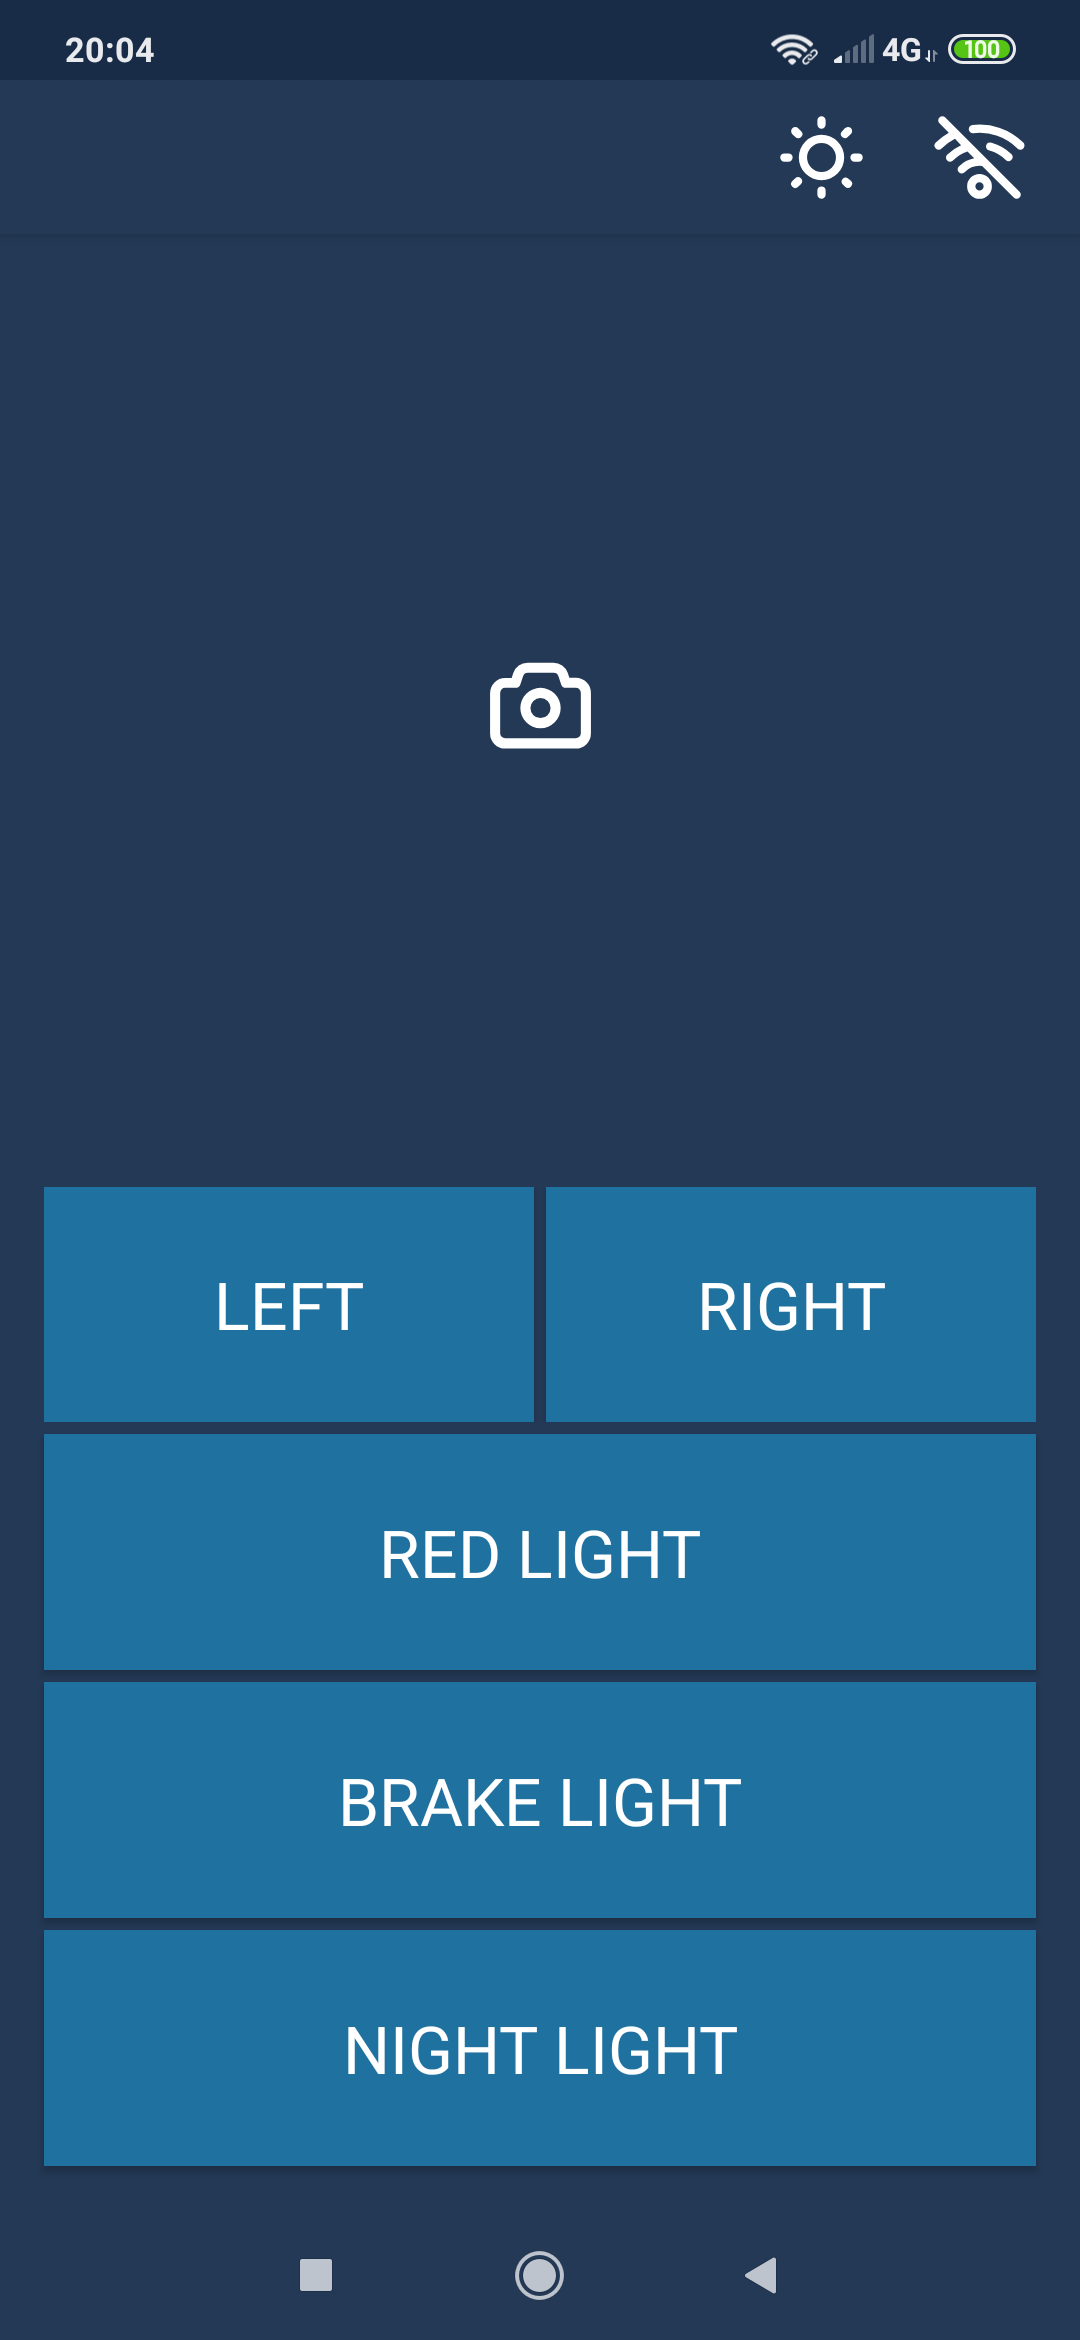
\includegraphics[scale=.1]{imaxes/layout-vertical1.png}
  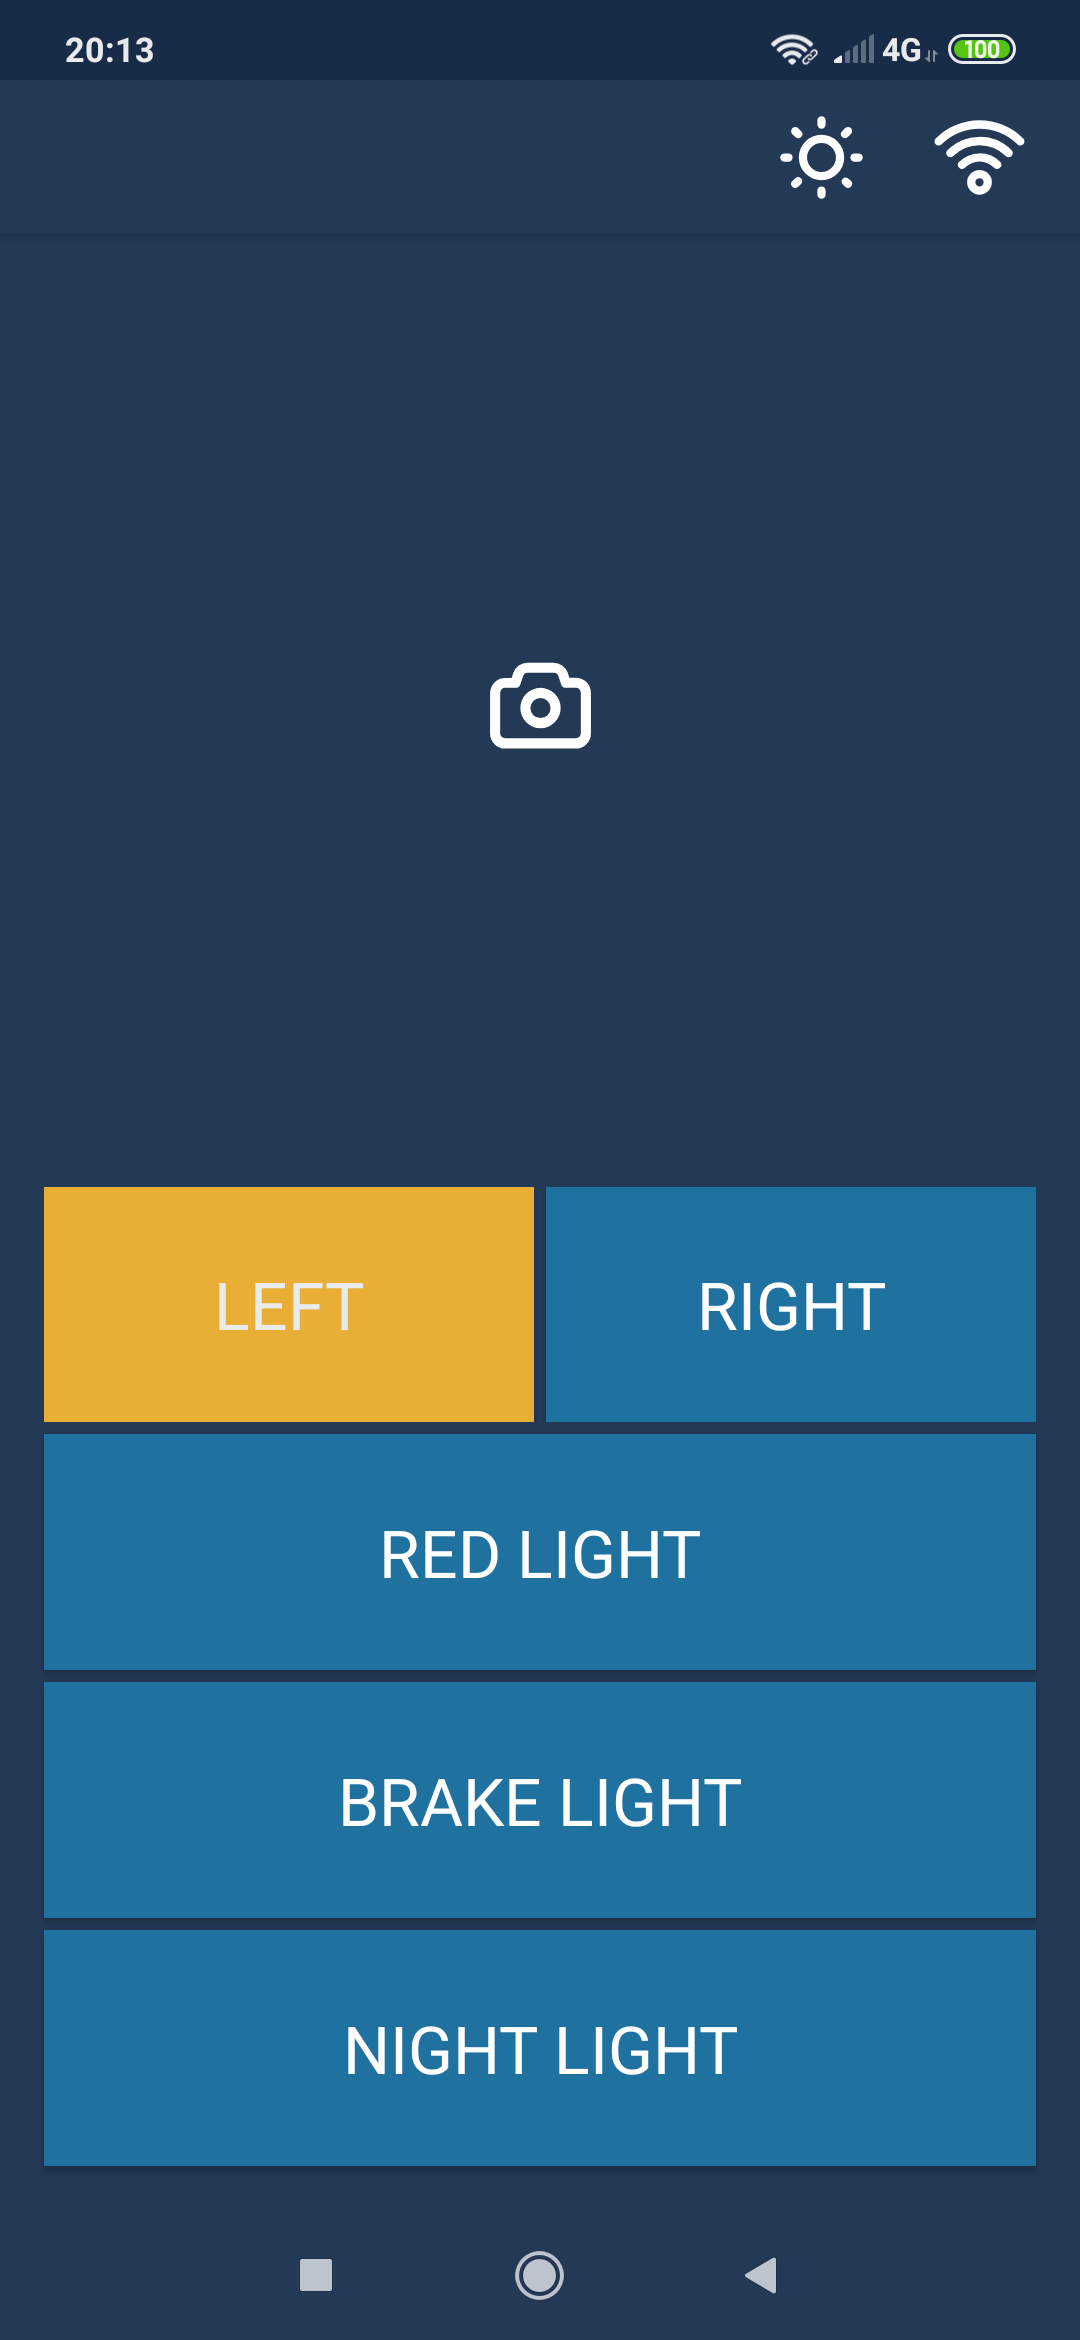
\includegraphics[scale=.1]{imaxes/layout-vertical2.png}
  \caption{Capturas de pantalla do \emph{layout} horizontal.}
  \label{fig:layout_horizontal}
\end{figure}
\subsubsection{Layout horizontal}
Neste \emph{layout}, figura~\ref{fig:layout_vertical}, o vídeo mostrarase como o fondo e os botóns sobre el. Os de xiro a esquerda e xiro dereita situados a ámbolos dous lados e o resto incluíndo o de control de intensidade lumínica e o de conexión situaranse na parte de inferior da pantalla.
\begin{figure}[tb]
  \centering
  
\includegraphics[scale=.1]{imaxes/layout-horizontal1.png}
  
\includegraphics[scale=.1]{imaxes/layout-horizontal2.png}
  \caption{Capturas de pantalla do \emph{layout} vertical.}
  \label{fig:layout_vertical}
\end{figure}
\subsection{Ciclo de vida da actividade}
En Android cada actividade conta conta cun ciclo de vida, figura~\ref{fig:actividade}, pasa por varios estados dende antes de iniciarse ata despois de finalizar. O estado principal dunha actividade é activa, no momento que a actividade está en primeiro plano e interactuando co usuario.

\begin{figure}[tb]
  \centering
  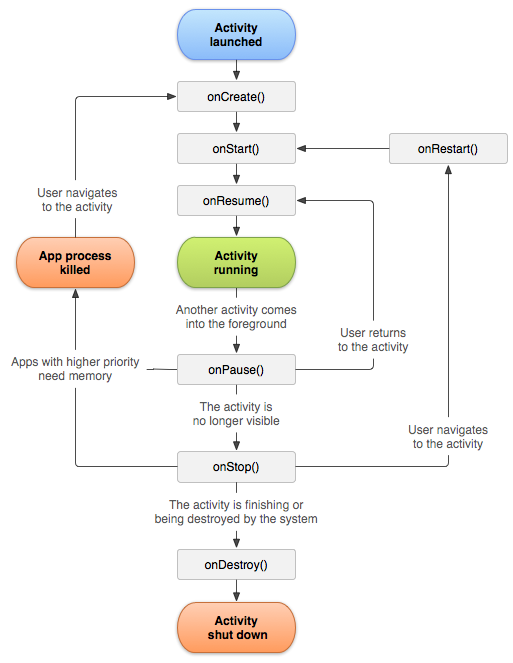
\includegraphics[scale=.6]{imaxes/ciclo-actividade.png}
  \caption{Ciclo de actividade Android~\cite{UnderstandActivityLifecyclea}}
  \label{fig:actividade}
\end{figure}

Para xestionar o que sucede no resto de estados utilízanse unhas funcións de \emph{callbacks}, no noso caso realizarase as seguintes accións en cada fase:
\subsubsection{onCreate}
Este método e o que se chama ao executar a actividade. Nel iniciarase os compoñentes a mostrar en pantalla e definirase o seu comportamento.

Aquí xestionarase o estado da conexión, iniciando a clase \emph{request} se non esta en funcionamento e enviando mensaxes o dispositivo para comprobar que segue conectado. Tamén xestionarase o estado da transmisión de vídeo xa que será necesario iniciar a recepción antes de iniciar a transmisión.
\subsubsection{onResume}
Este método executase despois de \emph{onCreate} cando a pantalla xa é visible para o usuario.

Rexistrarase aquí un \emph{sensor listener} para obter a información do sensor de luz.
\subsubsection{onPause}
Este método executase cando a aplicación deixa de estar en primeiro plano, se o usuario a minimiza u outra aplicación executase a actividade pasará a \emph{onStop} se despois de acceder a aplicacións recentes a aplicación volve a primeiro plano pásese o método \emph{onResume}.

Levarase a cabo neste método a cancelación do rexistro do sensor xa que non se seguira a utilizar e deterase a transmisión de vídeo se estase a executar.
\subsubsection{onDestroy}
Neste método a actividade e detida completamente e devénse liberar os recursos.

Aquí enviarase a orde para deter a conexión co dispositivo.

\subsection{Botons}
A actividade é a encargada de iniciar os botóns e manexar o seu funcionamento. Estes botón son os seguintes:
\begin{itemize}
    \item \textbf{Esquerda:} O pulsar este botón enviarase unha orde de acender a luz de xiro a esquerda. Se hai algunha luz acesa se enviará primeiro unha orde para apagalas. O pulsalo por segunda vez se enviara a orde de apagar luz de xiro e no caso de que a luz vermella estivese acesa antes de indicar o xiro esta luz se acenderá de novo. O botón palpebrará en amarelo mentres estea aceso.
    \item \textbf{Dereita:} O seu funcionamento é o mesmo que no botón esquerda.
    \item \textbf{Vermello:} O pulsalo enviarase unha orde para acender a luz de vermella, o pulsador non funcionara se algunha das luces de xiro está acesa.
    \item \textbf{Noite:} O pulsalo activarase o modo noite, no que o sensor lumínico do móbil encargarase de acender a luz vermella cando a luz ambiente baixe de certo umbral.
    \item \textbf{Freo:} Activa o modo de freada no que acenderase a luz vermella progresivamente cando o acelerómetro do dispositivo móbil detecte unha redución súbita na velocidade.
    \item \textbf{Brillo:} Este botón despregará unha barra cun indicador que poderase deslizar para elixir a intensidade das luces.
    \item \textbf{Conexión:} Este botón enviará unha orde de conexión, unha vez conectado cambiará a súa aparencia para indicar que existe conexión co dispositivo.
\end{itemize}
\subsection{Sensores}
Unhas das vantaxes de utilizar un dispositivo móbil é que estes contan con diversos sensores para moitos fins. No noso caso utilizarase o acelerómetro e o xiroscopio para rexistrar cambios na posición e aceleracións no dispositivo e o sensor de luz para medir a intensidade de luz no ambiente.
En Android accedese o sensor instanciando a clase \emph{SensorManager} e definindo unha instancia do sensor da que obterase os datos mediante a función \emph{on sensor change}~\cite{Sensors}.

\subsubsection{Sensor de Luz}
O sensor de luz é un fotorreceptor que xera unha sinal eléctrica dependendo da incidencia de fotóns. Para utilizar o sensor rexistrarase un \emph{sensor listener} no método \emph{onResume} e o método de \emph{callback} \emph{onSensorChanged} executarase cada vez que se detecte un cambio, neste método definirase o comportamento do sensor: Cando o botón de Noite esta activado acenderase o botón Vermello se o sensor rexistra un valor inferior a 400 lúmenes. Este valor correspondese coa intensidade lumínica o comenzo do solpor~\cite{Lux2019}.

\subsubsection{Acelerómetro e xiroscopio}
Para poder indicar a freada da bicicleta utilizarase o acelerómetro do dispositivo co que medirase a deceleración. O acelerómetro proporciona o valor da aceleración en $m/s^2$, para simplificar os cálculos utilizarase o sensor virtual \emph{ linear accelerometer} que proporciona o valor da aceleración excluíndo a gravidade asi o valor será 0 nos tres eixos cando o dispositivo este en repouso ou movéndose a unha velocidade constante.

A forza a obter é a deceleración no sentido da marcha, para poder calculala é necesario coñecer a orientación do dispositivo co respecto ao eixo lonxitudinal da bicicleta. O dispositivo situarase no guiador da bicicleta en dúas posición horizontal, ou vertical polo que en ámbalas dúas poderase excluír os valores dun dos eixos do acelerómetro, \emph{x} e \emph{y} respectivamente como se ve na figur~\ref{fig:angulo}. Para coñecer a influenza dos outros dous eixos sobre o plano paralelo a bicicleta necesitamos coñecer o ángulo que forma con esta. Utilizaremos o sensor virtual \emph{game rotation vector} para obter este ángulo, este sensor utiliza os datos do acelerómetro e o xiroscopio para proporcionar valores rotación en radiáns sobre os eixo de coordenadas da terra, aínda que non orientado o norte xa que este sensor virtual non utiliza o magnetómetro.  Estes valores están expresados en ángulos de Euler que indican mediante unha sucesións de xiros a desviación do sistema de coordenadas, para obter o ángulo respecto o eixo de coordenadas do móbil transformaremos o vector obtido mediante o calculo a matriz de rotación. Unha vez obtidos valores normalizados utilizaremos o ángulo respecto o eixo \emph{x} se o móbil esta en posición vertical e con respecto a \emph{y} se está en horizontal.

O ángulo obtido coincide co ángulo con respecto o eixo direccional da bicicleta so no caso no que a bicicleta estea sobre chan plano polo que será necesario que a bicicleta estea sobre un terreo sen inclinación, para elo o cálculo do ángulo realizarase nun proceso de calibración, cando se acenda o modo freada solicitarase que se coloque o telefono no soporte do guiador e se suxeite a bicicleta sobre un terreo chairo.
\begin{figure}[tb]
  \centering
  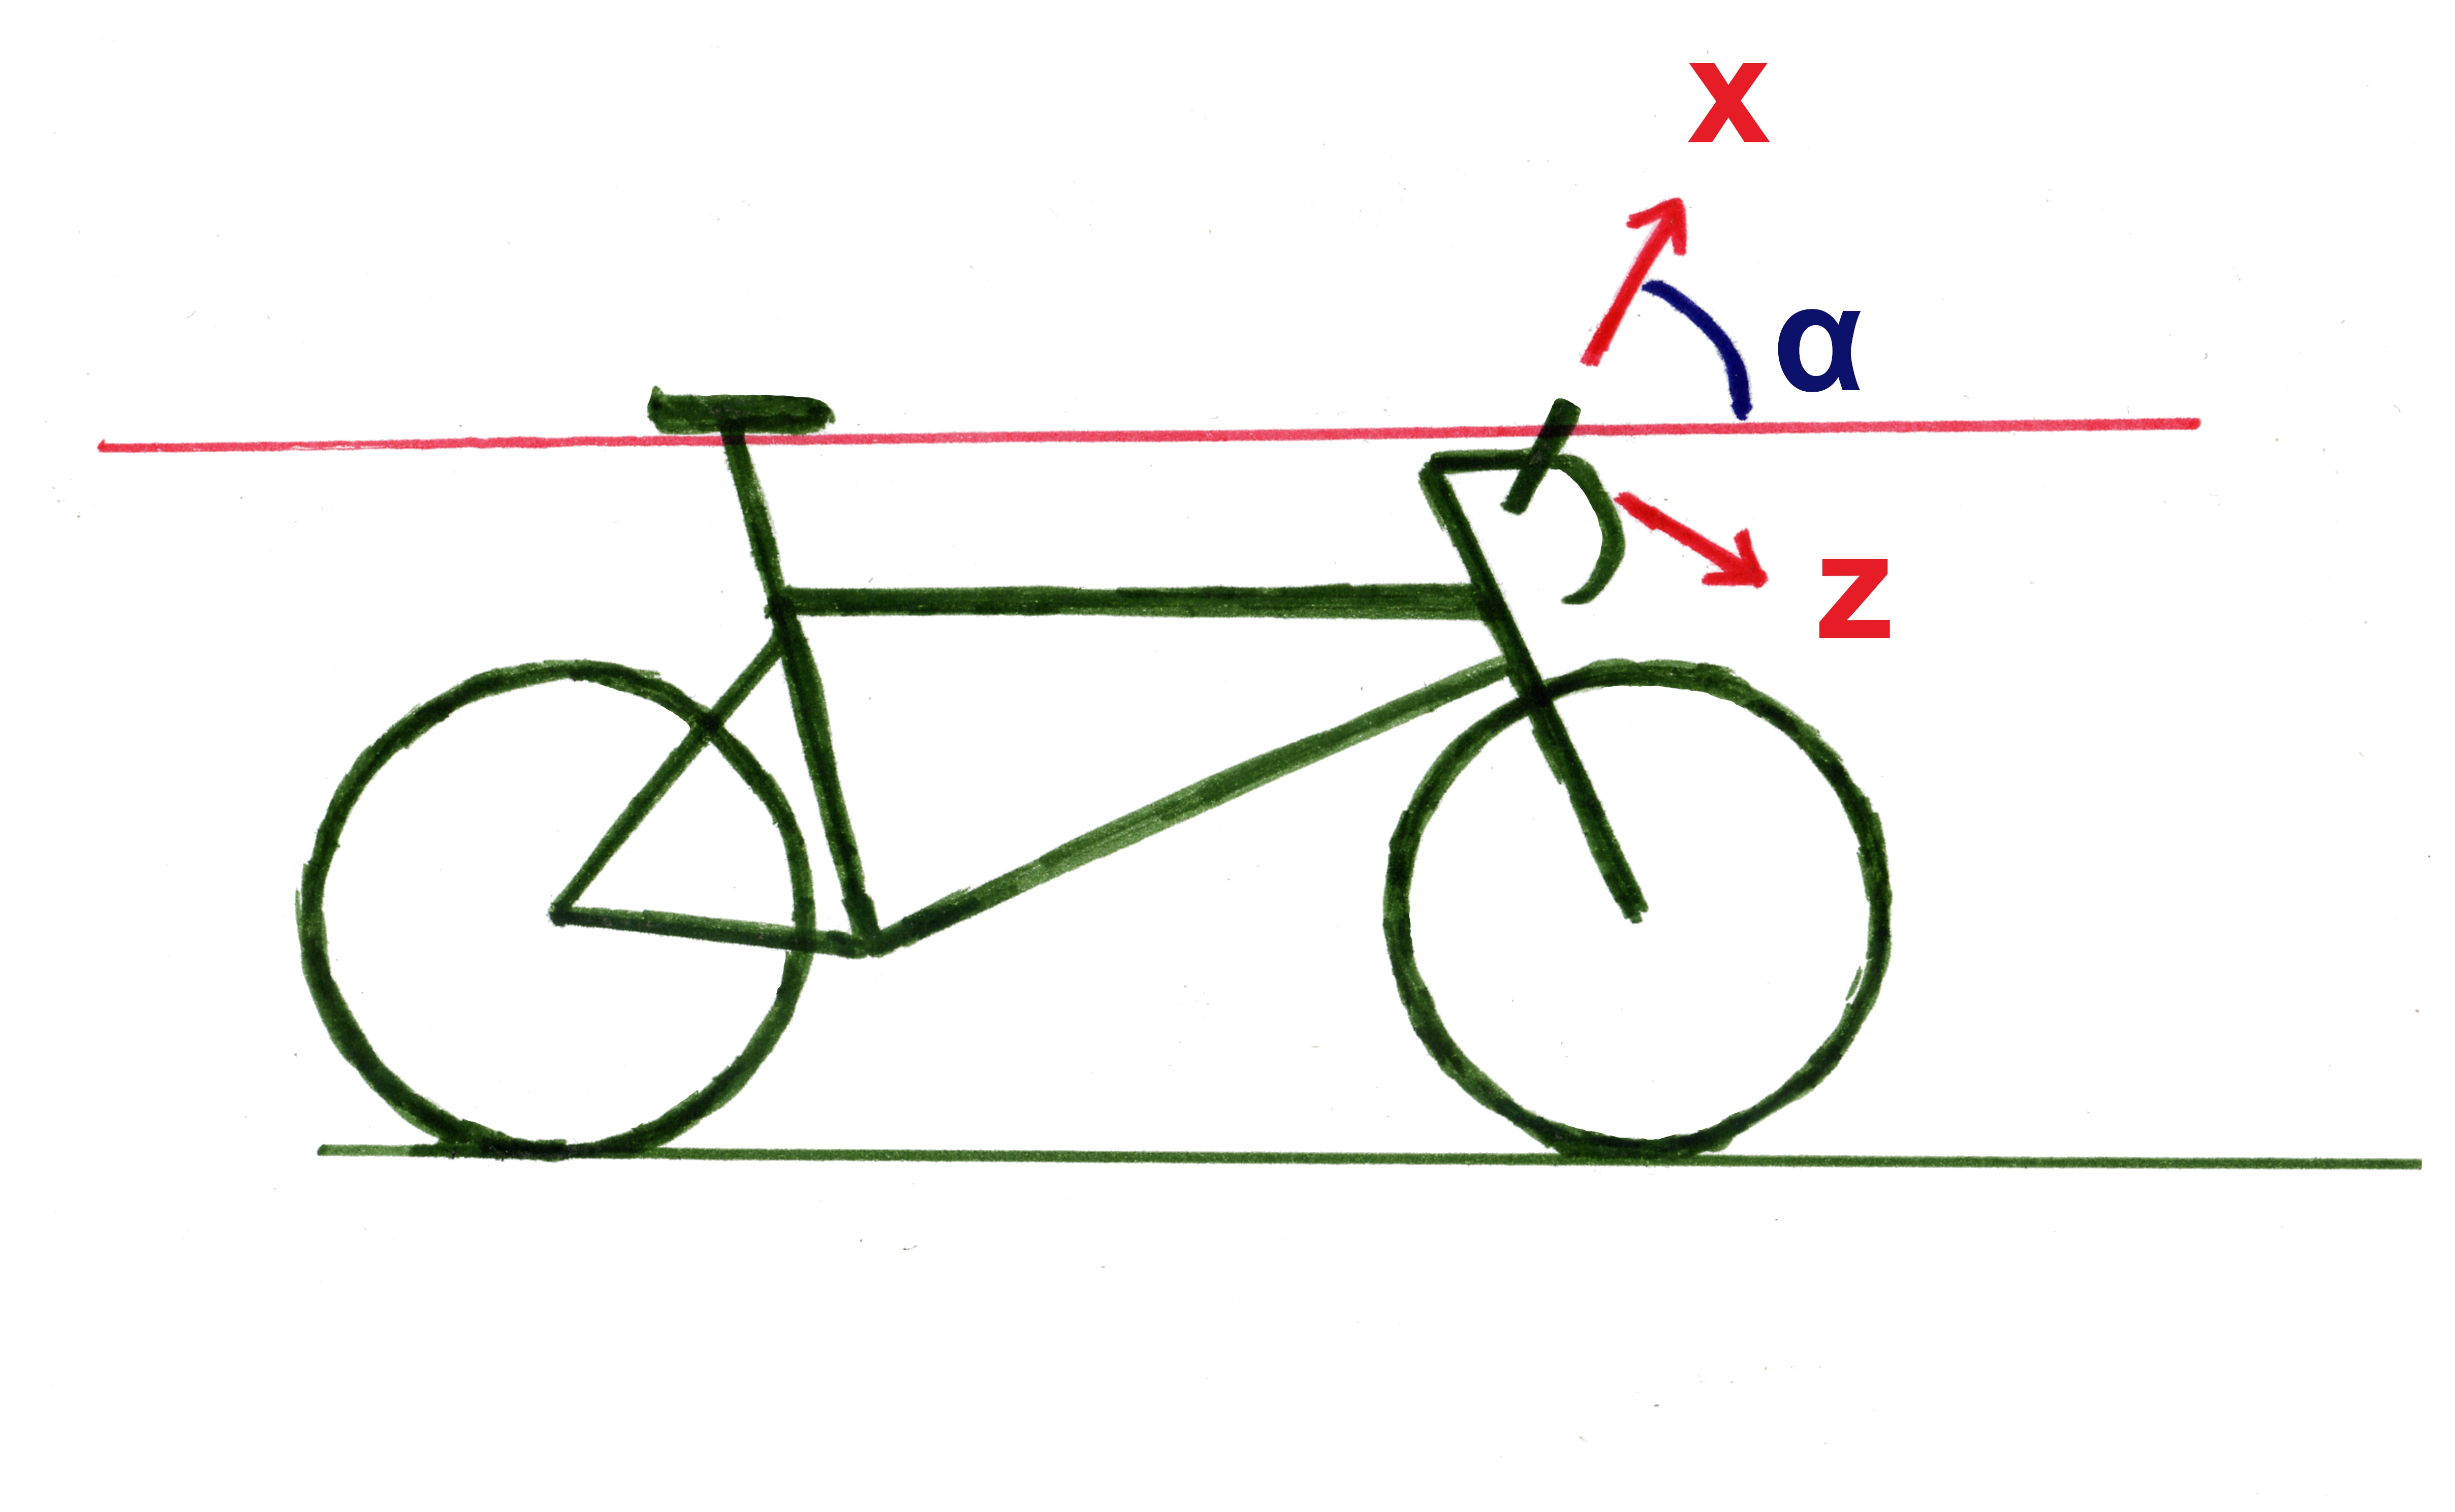
\includegraphics[scale=.6]{imaxes/angulo.png}
  \caption{Eixos do acelerómetro e ángulo coa horizontal. Para o dispositivo colocado en horizontal, en vertical o eixo superior sería \emph{y}.}
  \label{fig:angulo}
\end{figure}

O modulo da forza resultante calcularase de forma trigonométrica a partir dos valores de aceleración dos dous eixos e o ángulo obtido. O sistema indicará que se acenda as luces cando o valor calculado supere certo nivel, utilizarase en principio o valor de $m/s^2$ e comprobarase nas probas se é o valor adecuado.

De igual forma que no sensor de luz estes sensores rexistraranse no método \emph{onResume} e os cálculos cos valores obtidos realizaranse no método \emph{onSensorChanged}.

\subsection{Superficie de vídeo}
Iniciarase a superficie de vídeo na fase de creación da aplicación, procederase a reflectir a superficie para facer un efecto de espello para facer máis natural a a visualización do vídeo. O vídeo asignarase a superficie iniciando a clase \emph{VideoReceiver} mediante as funcións de \emph{callback} que se executarán cando se produza un cambio na superficie de vídeo.

\section{Comuniciacíon co dispositivo}
Crearase unha clase \emph{Request} encargada de tódalas comunicacións co dispositivo.  Esta clase, unha vez instanciada, encargarase de establecer a conexión co dispositivo, reconectar se se perde a conexión e transmitirlle as ordes.

\subsection{Broadcast}
Para coñecer a dirección IP do servidor, a clase \emph{request} conta cunha función que abrirá un socket no porto 5555 para esperar a recepción dun datagrama broadcasteado a tódalas direccións. O recibir o datagrama comprobase que conten a mensaxe \emph{"BikeView"} se é asi a función devolverá a dirección IP emisora do paquete.

\subsection{Conexión}
Unha vez obtida a dirección IP a clase \emph{request} utilizará unha función para establecer a conexión que devolverá un socket conectado ao socket remoto do servidor.

\subsection{Transmisión de ordes}
Para transmitir as ordes a clase \emph{request} contara cunha función que recibe a mensaxe a transmitir e a envía a través do socket. Espera a recibir resposta do servidor e se é positiva devolve o valor booleano verdadeiro, en caso de non recibila devolve o valor falso.

\section{Recepción de vídeo}
Para este apartado crearase a clase \emph{VideoReceiver} que executarase no seu propio \emph{thread}. O vídeo é codificado no formato H.264 e transmitido por UDP, para recibilo ábrese un \emph{socket} no porto 5000 extraese a mensaxe do datragrama e, para acelerar o proceso, en vez de utilizar a función \emph{MediaExtractor} pásase a unha función de parseo~\cite{consti10ContributeConsti10MyMediaCodecPlayerforFPV2018a} encargada de separar os datos recibidos en \emph{NAL units}, o formato que utiliza H.264 para o transporte. Para elo cando se identifica a cabeceira da seguinte \emph{NAL units} a anterior se envía a outra función encargada de decodificar o vídeo mediante un \emph{MediaCodec}~\cite{MediaCodec}, finalmente o vídeo mostrase na superficie.

\section{Anclaxe a bicicleta}
Existen diversas opcións paras suxeitar o móbil o guiador dunha bicicleta, no mercado hai soportes para dispositivos concretos e outros que se adaptan ao tamaño e forma de diferentes modelos. Neste caso utilizarase unha código \emph{SCAD} que ao executalo co software de deseño 3D paramétrico OpenSCAD no que introdúcense as dimensións do dispositivo e como resultado obtense un arquivo \emph{STL} co deseño 3D do soporte, figura~\ref{fig:soporte_mobil}.
\begin{figure}[tb]
  \centering
  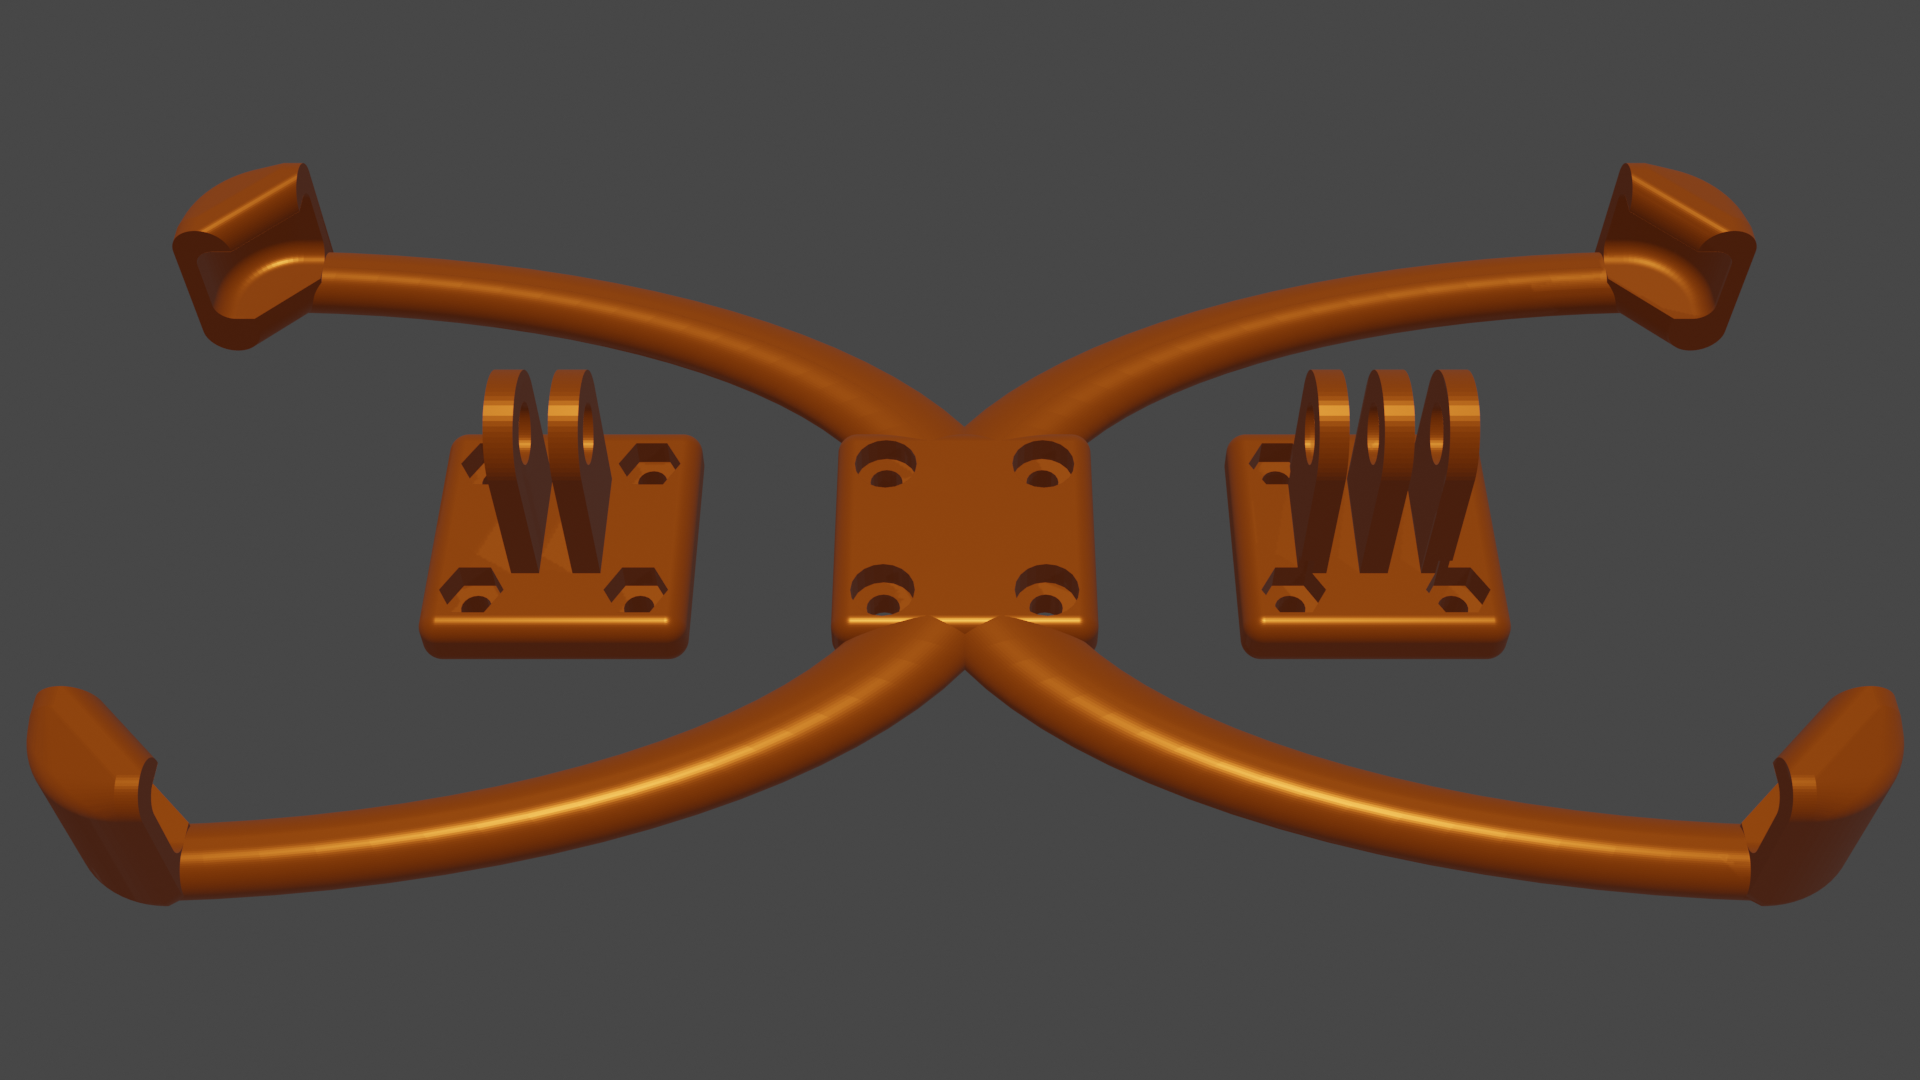
\includegraphics[scale=.2]{imaxes/soporte-mobil.png}
  \caption{Desño 3D do soporte para o dispositivo móbil.}
  \label{fig:soporte_mobil}
\end{figure}
Vendo que os soportes impresos non constaban coa resistencia esperada, como se mostra nas imaxes da figura~\ref{fig:fallos_soporte}, optouse por utilizar un soporte de aluminio nas probas para preservar a integridade do dispositivo móbil.
\begin{figure}[tb]
  \centering
  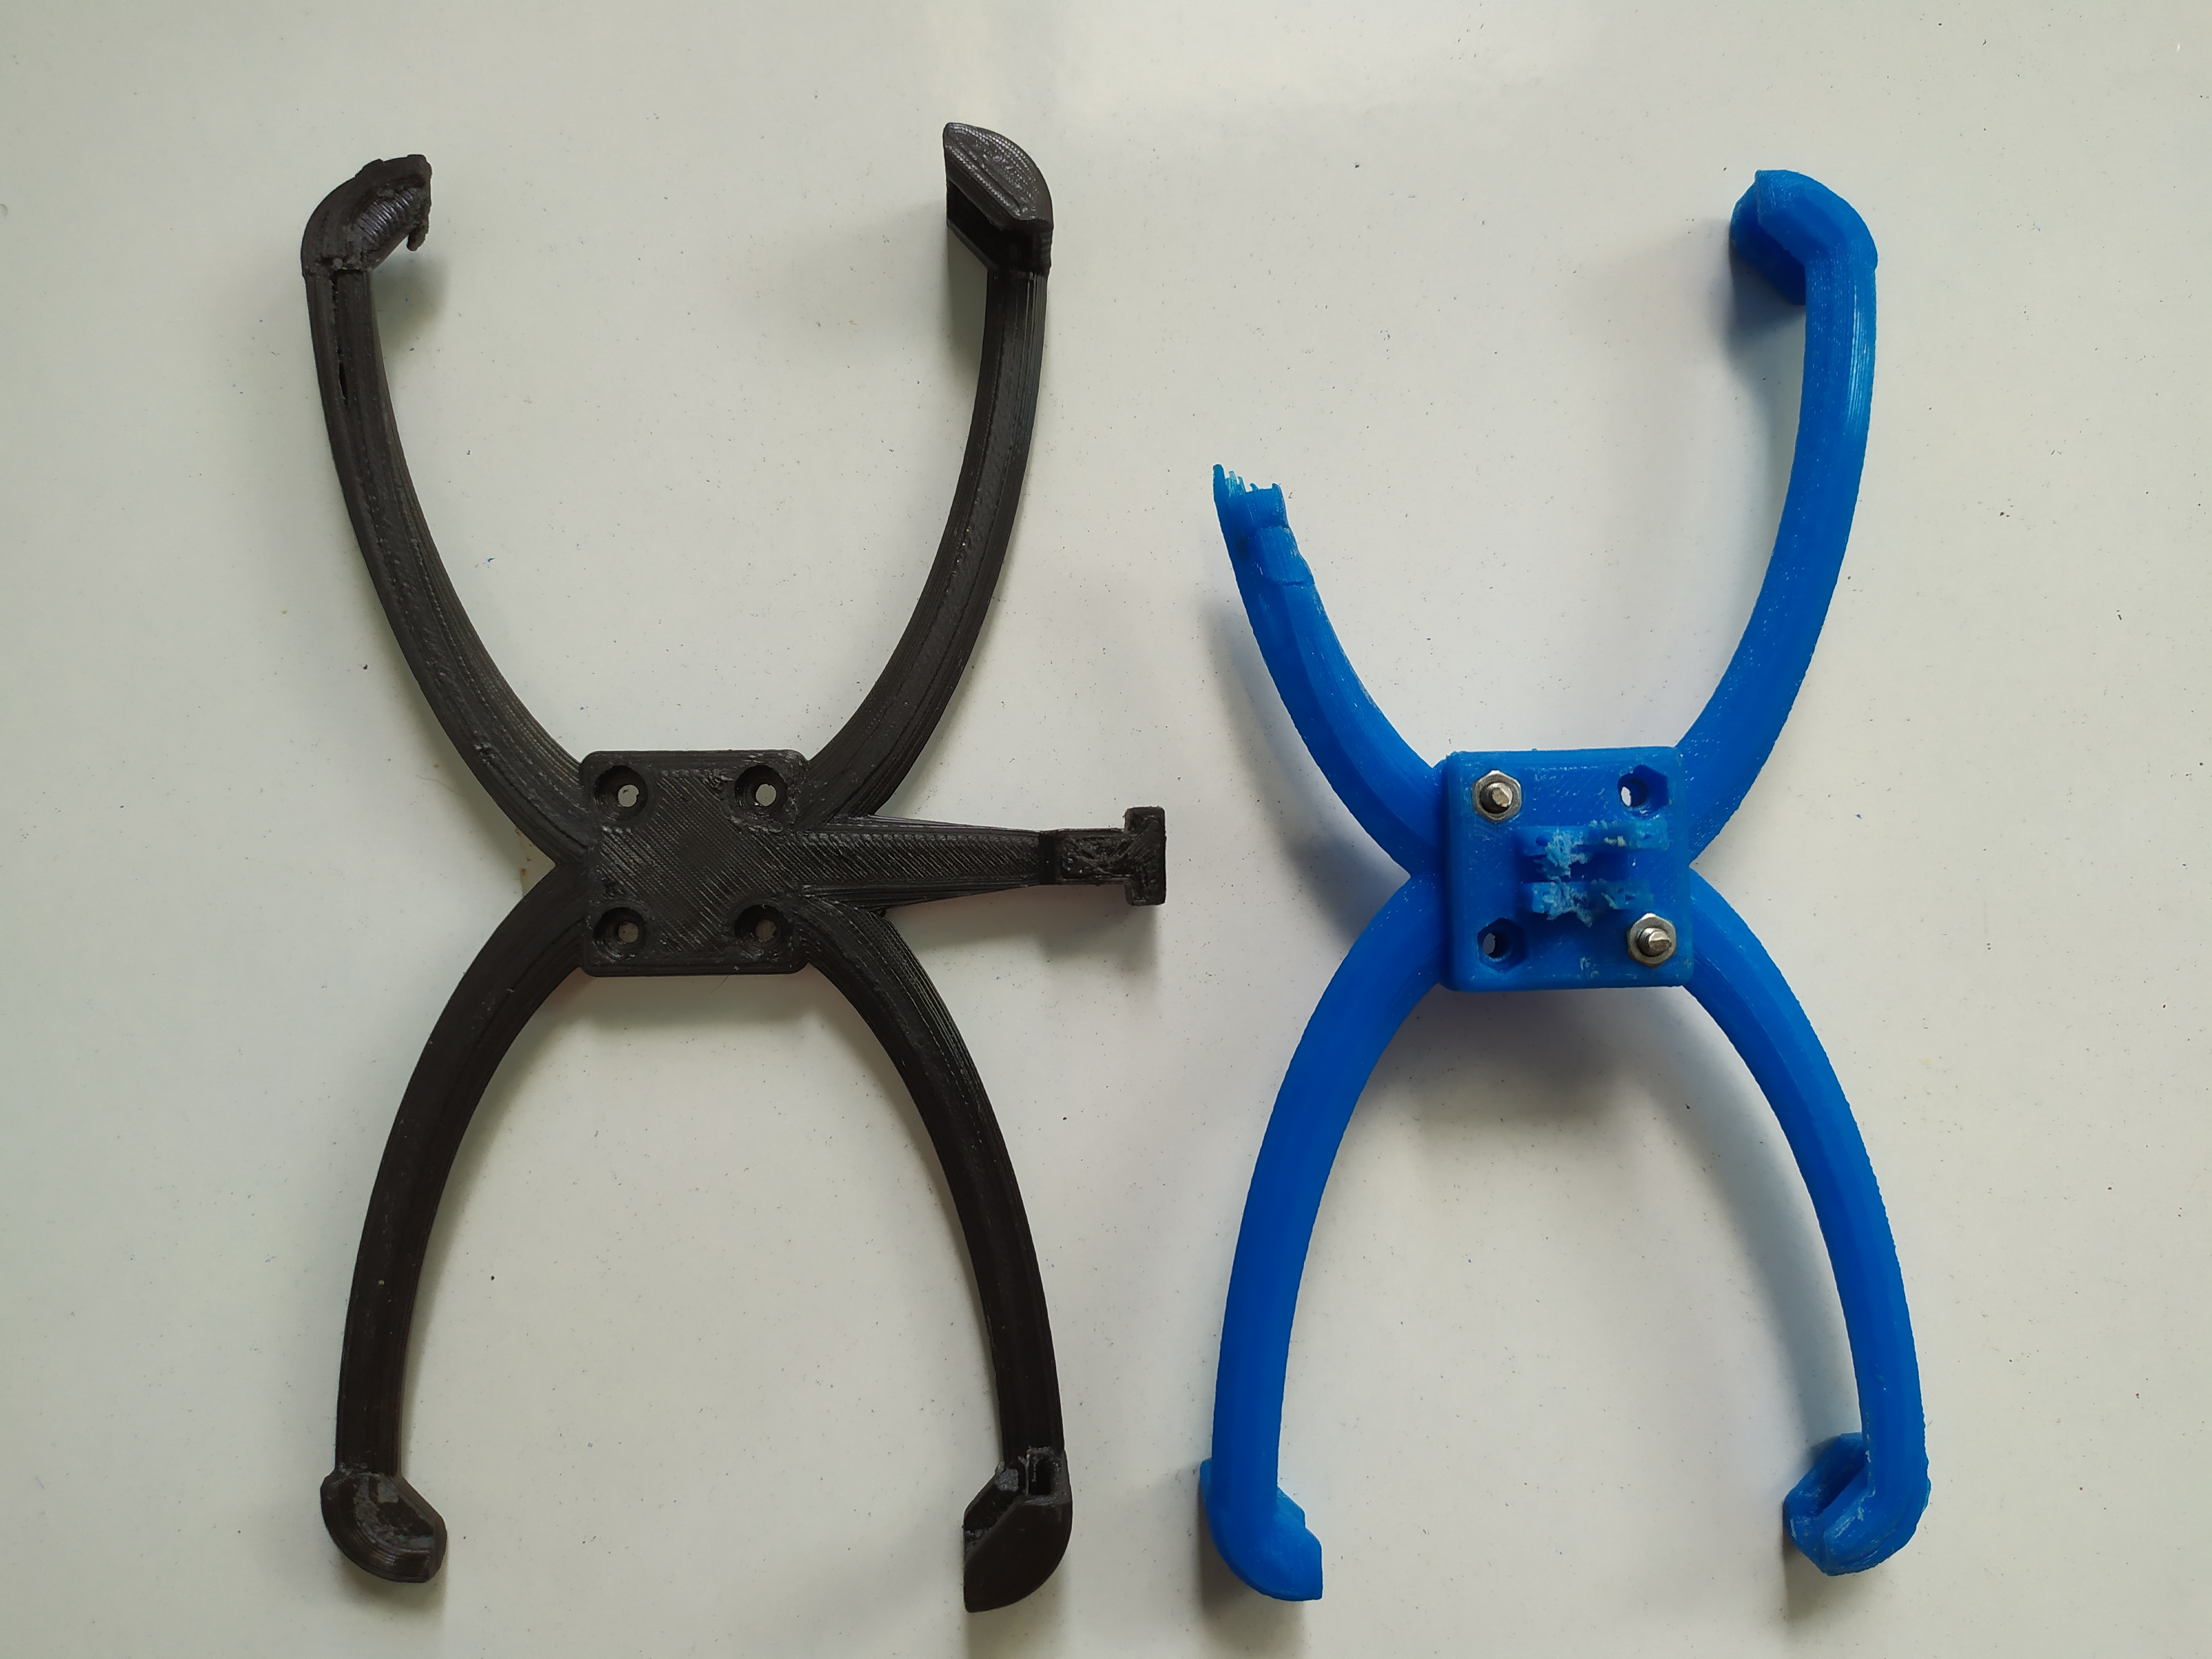
\includegraphics[scale=.08]{imaxes/fallos-soporte.jpg}
  \caption{Mostras dos problemas do soporte impreso.}
  \label{fig:fallos_soporte}
\end{figure}

 \chapter{Evaluación experimental}
\label{chap:evaluacion_experimenal}
Para comprobar que os resultados obtidos correspóndense co plantexado probaremos o dispositivo e a aplicación. Realizaremos probas en contornos controlados e probas no medio real o que esta dirixido e analizaramos a se cumpre os requisitos legais.

\section{Consumo e autonomía}

Comenzarase as probas medindo o consumo de amperios do sistema. Para elo colocarase un amperímetro usb entre unha fonte de alimentación e a conexión usb coa que alimentarase o sistema nestas probas. Repetiremos as probas con diferentes fontes de alimentación e distintos cables para descartar fallos e conseguir unha maior consistencia nos resultados. A continuación realizaranse as mesmas probas no dispositivo medindo o consumo alimentándoo coa batería.

Analizaranse os seguintes supostos para o dispositivo con un anel led e para o que conta a maiores coas dúas tiras led.
\begin{itemize}
    \item \textbf{Sistema en repouso: }
    O sistema esta aceso pero só se estean a executar as funcións do sistema operativo incluíndo o servidor ssh para o control remoto.
    \item \textbf{Servidor funcionando:}
    Executamos o servidor.
    \item \textbf{Cliente conectado:}
    Conectamos o dispositivo móbil o servidor.
    \item \textbf{Vídeo transmitindo:}
    Transmitimos vídeo en directo o dispositivo móbil.
    \item \textbf{Vídeo parado:}
    Paramos a transmisión de vídeo.
    \item \textbf{Desconexión do cliente:}
    Pechamos a aplicación no dispositivo móbil.
    \item \textbf{Luces intermitentes:}
    Iniciamos as luces intermitentes a máxima intensidade nunha das direccións, consumo varia no proceso, rexistremos o valor máximo.
    \item \textbf{Luces vermellas:}
    Acendemos as luces vermellas a intensidade máxima.
    \item \textbf{Luces vermellas e transmisión de vídeo:}
    Consumo coas luces vermellas a máxima intensidade e co vídeo transmitindo en directo.
\end{itemize}

\begin{figure}[tb]
  \centering
  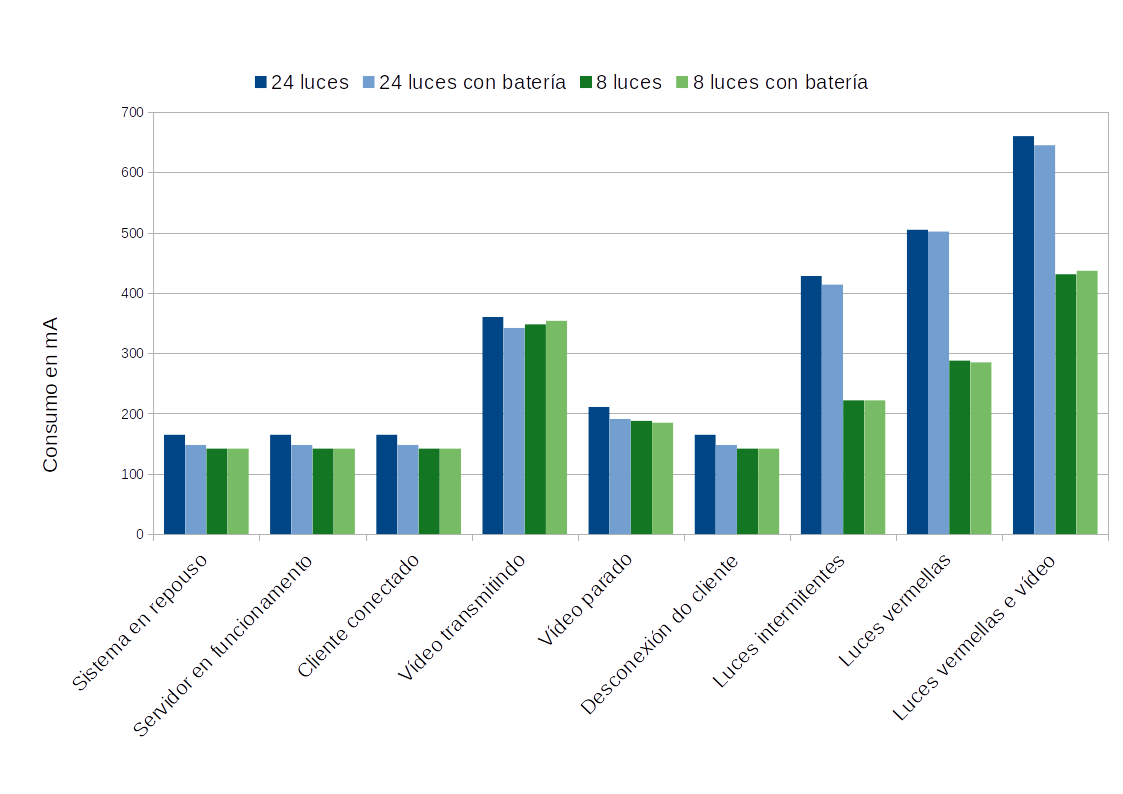
\includegraphics[scale=.5]{imaxes/grafica-amperaxe.png}
  \caption{Grafica do consumo en mA.}
  \label{f:soporte móbil}
\end{figure}
Como se pode observar na gráfica da figura 5.1 o uso ou non de batería non afecta en gran medida ao consumo de amperios, pero ha de terse en conta que estas probas realizáronse coas batería coa carga completa. Se se compara a previsión de consumos feita coas medición obtidas
pódese ver que os valores no son moi diferentes sendo superior no caso do dispositivo de 8 luces, 437mA fronte aos 390mA previstos, e inferior no caso dispositivo con 24 luces, 660mA fronte aos 710mA previstos.
As fontes de alimentación utilizadas poden proporcionar un máximo de 3A e 2.1A respectivamente, tamén utilizáronse dous cables un de maior calidade e outro cunha calidade inferior. En ningún dos casos obtivéronse diferencias apreciables sendo a maior diferencia de 4mA. Na versión con batería necesitouse utilizar cableado a maiores para realizar as probas, o que pode que incrementara lixeiramente o consumo.

A seguinte proba a realizar será a de autonomía do dispositivo, para elo buscarase o consumo máximo acendendo as luces vermella a máxima intensidade o tempo que se transmite vídeo.

Comezaranse as probas co dispositivo dotado de batería interna, cando a voltaxe da batería esta entorno os 3.7V detectase un problema o sistema apagase, indicando batería baixa. O \emph{script} Python encargado de monitorizar o pin conectado o indicador de voltaxe baixo do Adafruit Powerboost detecta unha caída de voltaxe que confunde co franco de caída esperado cando o pin ponse a 0. O pin de baixo voltaxe do Adafruit Powerboost está conectado a voltaxe da batería cando a caga e superior a 3.2V e conectase a un valor de 0V cando baixa de este limite e debido a que cando batería esta a comezar a descargarse para poder proporcionar a amperaxe adecuada a súa voltaxe baixa a un ritmo rápido que confunde o \emph{script}. O podemos solucionar incluíndo unha segunda comprobación no \emph{script} despois de detectar o franco de caída comprobarase que o valor lido no pin é 0 antes de apagar a Raspberry.

A continuación detectase un segundo problema, despois de  min volvese a apagar por batería baixa e unha vez apagado a batería recuperase ata unha voltaxe de 3.5V. Esto debese a que o estar consumindo o máximo de amperios necesita baixar a súa voltaxe para poder seguir entregando estes amperios. Que o sistema se apague neste punto e conveniente para protexer a batería e prolongar a súa vida útil pero reduce o tempo de uso da batería, que poderíamos seguir usando sempre que non utilicemos o consumo máximo do dispositivo. Este problema pódese solucionar de dúas formas:
Utilizando un batería de maior capacidade xa que poderá seguir subministrando a amperaxe necesaria a menor voltaxe.
Utilizar unha batería cunha constante de descarga maior, isto é a capacidade máxima de amperios que pode subministrar en función da capacidade en amperios hora. A batería utilizada ten unha constante de descarga de 1C isto quere dicir que coa sua caga completa o fabricante garante que proporcione 1.6A funcionando con normalidade.
Ámbalas dúas solucións implican na practica unha batería de maior tamaño.

Procedemos a repetir a proba pero esta vez deshabitando o apagado automático, esperando a que o sistema se apague cando a voltaxe non sexa suficiente para manter a Raspberry acesa ou no peor caso cando o circuíto de protección que inclúe a batería a desconecte a 2.5V. De non usar unha batería con circuíto de protección poderíamos danar a batería podendo incluso arder ou estoupar durante próximas cargas. Neste caso obtemos minutos de funcionamento.

Comezarase as probas para a versión do dispositivo sen luces intermitentes, faremos a proba cunha batería de  mA, obtense    , Neste caso observase que cando o dispositivo non pode subministrar suficiente voltaxe para alimentar a Raspberry esta se apaga, e como consecuencia tamén os leds alimentados dende o seu \emph{power rail}, o diminuír o consumo a voltaxe volve a ser suficiente para alimentar a Raspberry polo que esta se reinicia, entrando desta forma nun ciclo de reinicios ata que a voltaxe non e suficiente para arrancar a Raspberry.

\section{Vídeo e lentes}
Nesta sección procederase a analizar a calidade do vídeo obtida a latencia
\section{Visibilidade}

\section{Estabilidade e consumo da aplicación}

\section{Lexislación}
A Lexislación que regula o uso de luces e cámaras varía amplamente segundo o país, analizaremos a legalidade do dispositivo segundo a lexislación española.
\subsubsection{Luces}
O uso de luces en bicicleta e obrigatorio en España cando as condicións lúminicas son insuficientes, na Instrución 18/S-146 da Dirección Xeneral de Tráfico con respecto a legalidade de luces parpadeantes, detalla os requisitos lumínicos aplicables as bicicletas recollidos nas diferentes lexislacións (incluir cita):
\begin{itemize}
  \item Artigo  98.1  do  Regulmento  Xeneral  de Circulación, aprobado por Real Decreto 1428/2003, de 21 de novembro.\\
  "Todos los vehículos que circulen entre el ocaso y la salida del sol o a cualquier hora del día en los túneles, pasos inferiores y tramos de vía afectados por la señal “túnel” (S-5) deben llevar encendido el   alumbrado   que   corresponda   de   acuerdo   con   los   que   se determina en esta sección".
  \item  Regulamento Xeneral de Vehículos, aprobado por Real Decreto 2822/1998, de 23 decembro\\
  "En el artículo 22.4 se indica que las bicicletas, para circular de noche, por tramos   de   vías   señalizados   con   la   señal   de   “túnel”   o   cuando   existan condiciones  meteorológicas  o  ambientales  que  disminuyan  sensiblemente  la visibilidad,  deberán  disponer  de  los  siguientes  dispositivos: luz  de  posición delantera   y   trasera,   catadióptrico   trasero,   y   podrán   disponer   de catadióptricos en los radios de las ruedas y en los pedales".
  \item Real Decreto 339/2014, de 9 de mayo, que establece os requisitos para a comercialización e posta en servizo das bicicletas e outros ciclos e as súas partes e pezas,establece no Anexo V o rango de intensidade lúmica nos faros das bicicletas.
  \begin{figure}[h!]
    \centering
    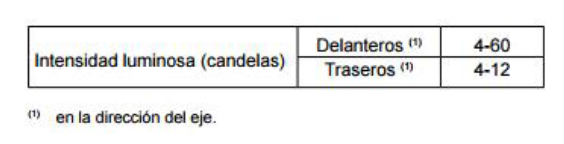
\includegraphics[scale=0.6]{imaxes/lexislacion-luminica.png}
    \caption{Rango de intensidade luminica nos faros das biciletas en España.}
    \label{f:lexislación lumínica}
  \end{figure}
\end{itemize}
A instrución conclúe que o uso de luces parpadeantes é legal sempre que as luces no produzan cegamento o resto de usuarios da vía e se adecúen a normativa citada.//
Para saber se as luces cumpren estes requisitos lumínicos tense que calcular as candelas que emiten. Os fabricantes de tiras leds raramente indican esta información e se o fan é en formato de lúmenes que para converter a candelas e necesario saber o ángulo de emisión, dato que tampouco facilitan, e non tódolos leds co mesmo formato compórtanse da mesma maneira. Na ficha técnica duns leds WS2812B, coma os utilizados neste proxecto, do fabricante Worldsemi (incluir referencia) na táboa 6.1 especifican as milicandelas dos seus leds, tendo unha intensidade lumínica máxima combinada de entre 1850 e 2500 milicandelas.

O dispositivo desenvolto so utiliza dúas cores a vermella cun valor \emph{RGB} (255,0,0) e a amarela cun valor \emph{RGB}  (255,170,0). Polo tanto para a luz vermella solo utilizamos este led cunha intensidade máxima indicada na táboa deste fabricante de entre 550 en 700 milicandelas. Para a luz amarela o led vermello funciona a intensidade máxima e o verde cun valor de 177 dun máximo de 255, supoñendo unha transmisión lineal destes valores a intensidade en candelas, obteríase un valor do 69.4\(\%\) que sobre os datos do fabricante para o led verde resulta entre 763 e 961 milicandelas, sumados os valores do led vermello o resultado é un máximo de entre 1313 e 1661 milicandelas.

Para a luz vermella, no dispositivo de 8 luces isto serán entre 4.4 e 5.6 candelas, dentro do rango legal de entre 4 e 12 candelas, no caso do dispositivo de 24 luces o intensidade máxima será de entre 13.2 e 16.8 candelas en principio superior o limite legal non obstante este requirimento de intensidade é na dirección do eixo e as 16 luces extras utilizadas neste dispositivo están colocadas nun ángulo duns 55 graos polo que a intensidade na dirección será inferior, non e posible calcular este valor sen coñecer o ángulo de emisión de luz de estes leds.
Para a luz amarela entre 10.5 e 13.2 candelas, podendo ser neste caso superior o limite legal, no dispositivo de 24 luces o valor máximo será de entre 31.5 e 39.8 candelas aínda que de igual forma que as vermellas o valor na dirección do eixo será menor.

Como se pode observar en tódolos casos, a priori, as luces acadan o limite legal pero nalgúns o sobrepasan, para adaptar o comportamento das luces a lexislación bastará con limitar o valor da intensidade máxima. Para poder obter este valor será necesario realizar probas empíricas para medir as candelas emitidas polo dispositivo.

Cabe destacar que o uso de indicadores de xiro non está recollido na lexislación española polo que seu uso podería ser sancionable se considérase que  pode ser contraproducente cegando a visión doutros ocupantes da vía. O seu uso non eximirá a necesidade de indicar as manobras co brazo como require a lei.
\begin{table}[tb]
    \label{c:intensidade leds}
    \begin{center}
        \begin{tabular}{|l|l|l|l|l|}
            \hline
             Cor a emitir & Modelo & Lonxitude de onda (nm) & Intensidade lumínica (mcd)&Voltaxe(V)\\ \hline
             Vermello & 13CBAUP & 620-630 & 550-700 & 1.8-2.2\\ \hline
             Verde & 13CBAUP & 620-630 & 1100-1400 & 3.0-3.2\\ \hline
             Azul & 10R1MUX & 465-475 & 200-400 & 3.0-3.4\\ \hline
        \end{tabular}
    \end{center}
    \caption{Características dos leds WS2812B de Worldsemi}
\end{table}

\subsection{Cámaras}

 \chapter{Conclusións}
\label{chap:conclusions}

\lettrine{D}{erradeiro} capítulo da memoria, onde se presentará a
situación final do traballo, as leccións aprendidas, a relación coas
competencias da titulación en xeral e a mención en particular,
posibles liñas futuras,\dots
\section{Traballo futuro}
Mellorar interfaces da app, subila a tenda de aplicacións de google
Engadir mecanismos de control, control por voz, mando no guiador, pulsadores intermitentes
desear circuito impreso
Detector de caídas
Soporte a multiples dispositivos, visualizar diferentes camaras, utilidade en outros ambitos, camións etc.
Mellorar a estructura do dispositivo, facelo resistente a auga e golpes, protexer os leds,
Estudar a unclusion de difusores de luz e ou lentes nos leds para aumentar a distancia de visualización e oou reducir o Consumo
Luces frontais e laterais
Aumentar a bateria e o mecanismo de proteción desta para aumentar o tempo de uso
Apagar o dispositivo dende a aplicación
Engadir menú de configuriación
Carga rápida


 %%%%%%%%%%%%%%%%%%%%%%%%%%%%%%%%%%%%%%%%
 % Apéndices, glosarios e bibliografía  %
 %%%%%%%%%%%%%%%%%%%%%%%%%%%%%%%%%%%%%%%%

 \appendix
% \newpage
\chapter{Apéndices}
\thispagestyle{empty}

\chapter{Contido DVD}

\chapter{Requisitos e instalación}
Para a instalación do software no dispositivo BikeCam neceitaremos unha Raspberry Pi con unha tarxeta micro sd cuha capacidade mínima de 4GB.

Comezarase por descargar ultima versión de raspbian lite da web da Rasberry Pi e gravar a imaxe na tarxeta micro sd, isto pódese acadar mediante o comando \emph{dd} ou mediante unha ferramenta con ese propósito como balenaEtcher.
Unha vez finalizado accederase á partición boot coa que conta agora a tarxeta de memoria, nela crearemos un arquivo baleiro chamado ssh para activar a interface ssh cando o sistema arranque, creamos tamén nesta ubicación un arquivo chamado wpa\_supplicant.conf para configurar a conexón wifi, nel introducirmos os datos do SSID e a cotraseña da rede Wi-Fi creada polo dispositivo android

	country=COUNTRY

	ctrl\_interface=DIR=/var/run/wpa\_supplicant GROUP=netdev

	update\_config=1

	network={

	  \indent     ssid="SSID"

	   \indent    psk="PASSWORD"

	   \indent    key\_mgmt=WPA-PSK

	    }

Expulsamos a tarxeta e a introduciomos na Raspi Pi e a encendemos, dende un ordenador ou dispositivo móbil averiguamos a direción ip, con por exemplo o softwar Fing dispoñible para linux e android. Conectamonos por ssh co usuario e contraseña por defecto "pi" "raspberry", é altamente recomendable cabiar a cotnraseña por defecto co comando passwd.

Executamos sudo raspi-config e no apartado Interfacacing Options activar o modulo da cámara, no apartado advanced options executamos a opción enlage filesistem. A continuación executamos o apartado update, de seguido poderemos saír da raspi-config e actualizar o sitema cos comandos
sudo apt update e
sudo apt upgrade

Para instalar a librería  de jgarff para o control de los LEDs instalamos a seguinte aplicación sudo apt install scons
descargamos aa librería con

 wget \url{https://github.com/jgarff/rpi_ws281x/archive/master.zip}

descomprimimos con unzip master.zip
entramos na carpeta e executar o comando scons
executamos sudo apt install python-dev swig.

A continuación entramos na carpeta python e executamos sudo python ./setup.py build e a contunuación sudo python ./setup.py install

\newpage
\thispagestyle{empty}


 \chapter{Glosario de acrónimos}
\label{chap:acronimos}

%%%%%%%%%%%%%%%%%%%%%%%%%%%%%%%%%%%%%%%%%%%%%%%%%%%%%%%%%%%%%%%%%%%%%%%%%%%%%%%%
% Obxectivo: Lista de siglas, abreviaturas, acrónimos, etc. empregados         %
%            no documento, xunto cos seus respectivos significados.            %
%%%%%%%%%%%%%%%%%%%%%%%%%%%%%%%%%%%%%%%%%%%%%%%%%%%%%%%%%%%%%%%%%%%%%%%%%%%%%%%%

\begin{description}
 \item [LiPo] \emph{Lithium Polymer }.
 \item [SRAM] \emph{Static Random-access Memory}.
 \item [PWM] \emph{Pulse Width Modulation}.
 \item [SPI] \emph{Serial Peripheral Interface}.
 \item [UART] \emph{Universal Asynchronous Receiver/Transmitter}.
 \item [I2C] \emph{Inter-Integrated Circuit}.
 \item [FPGA] \emph{Field Programmable Gate Arrays}.
 \item [IoT] \emph{Internet of Things}.
 \item [RISC] \emph{Reduced Instruction Set Computer}.
 \item [RGB] \emph{Red Green Blue}.
 \item [CSI] \emph{Camera Serial Interface}.
 \item [PLA] \emph{Polylactic Acid}.
 \item [ABS] \emph{Acrylonitrile Butadiene Styrene}.
 \item [OTG] \emph{On the Go}.
 \item [FPS] \emph{Frames Per Second}.
 \item [UDP] \emph{User Datagram Protocol}.
 \item [TCP] \emph{Transmission Control Protocol}.
 \item [IP] \emph{Internet Protocol}.
 \item [HTTP] \emph{ HyperText Transfer Protocol}.
 \item [GPIO] \emph{General-prupouse Input/Output}.
 \item [NAL] \emph{Network Abstraction Layer}.

\end{description}

%%%%%%%%%%%%%%%%%%%%%%%%%%%%%%%%%%%%%%%%%%%%%%%%%%%%%%%%%%%%%%%%%%%%%%%%%%%%%%%%

 \chapter{Glosario de termos}
\label{chap:glosario-termos}

%%%%%%%%%%%%%%%%%%%%%%%%%%%%%%%%%%%%%%%%%%%%%%%%%%%%%%%%%%%%%%%%%%%%%%%%%%%%%%%%
% Obxectivo: Lista de termos empregados no documento,                          %
%            xunto cos seus respectivos significados.                          %
%%%%%%%%%%%%%%%%%%%%%%%%%%%%%%%%%%%%%%%%%%%%%%%%%%%%%%%%%%%%%%%%%%%%%%%%%%%%%%%%

\begin{description}
 \item [Bytecode] Código independente da máquina que xeran
   compiladores de determinadas linguaxes (Java, Erlang,\dots) e que
   é executado polo correspondente intérprete.
 \item [Lipo]
 \item [Toolchain] Conxunto de ferramentas encadeadas para desenvolver
 un produto de software.
 \item [Buffer] Memoria utilizada temporalmente para almacenar datos de
 entrada ou saída durante a transmisión.
 \item [Kernel] Nucleo do sistema operativo, encargado da xestión do resto
 de elementos do sistema.
 \item [Aliassing] Efecto que causa que dúas sinais diferentes sexa indistinguibles
 por falta de resolución de mostraxe.
 \item [Streaming] Retransmisión en directo dun contido ou sinal.
 \item [Bitstream] Secuencia de bits.
 \item [Socket] Interface para intercambiar un fluxo de datos nunha conexión.
 \item [Bitrate] Indica o numero de bits por unidade de tempo.
 \item [Thread] Secuencia de instrucións que pode ser manexada por un planificador
 como pode ser o sistema operativo.
 \item [STL] Stereolithography, formato de arquivo para a representación
 tridimensional da estrutura dunha figura .
 \item [GCODE] Linguaxe de programación para o control numérico.
 \item [Systemd] Conxunto de daemons de administración do sistema, utilizado
  varios sistemas Linux.
 \item [Log] Rexistro escrito dun evento.
 \item [Callback] Función pasada como argumento de outra, que permite aumentar
 a abstración do código.
 \item [Script] Programa escrito nunha linguaxe de scripting, que permite a execución
 de ordes nun intérprete sen necesidade de compilación previa.

\end{description}


 %\bibliographystyle{plain}
 \bibliographystyle{IEEEtranN}
 \bibliography{bibliografia/bibliografia}
 \cleardoublepage

\end{document}

%%%%%%%%%%%%%%%%%%%%%%%%%%%%%%%%%%%%%%%%%%%%%%%%%%%%%%%%%%%%%%%%%%%%%%%%%%%%%%%%
